\subsubsection[Refinement of the Use Case Manage Users \& Roles]{Refinement of the Use Case Manage Users \& Roles} Figure
\ref{fig:admin-manage-users-and-roles-use-case} presents the refinement of the
Use Case Manage Users \& Roles for the Administrator actor. This use case includes
the following sub-use cases:
\begin{figure}[H]
    \centering
    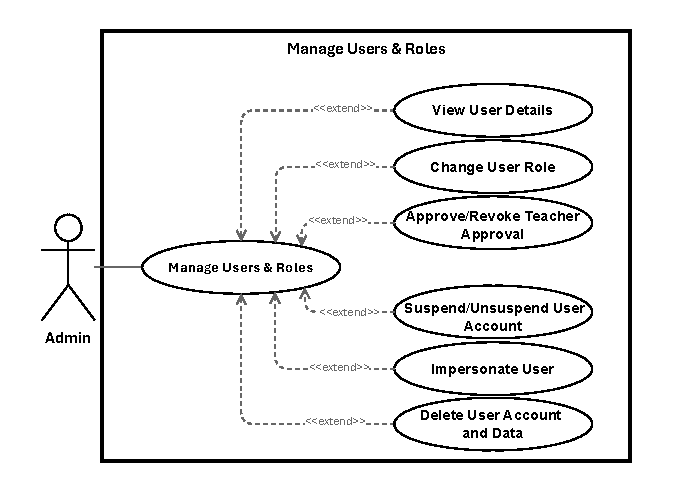
\includegraphics[width=\textwidth]{assets/chapter3/admin-manage-users-and-roles-use-case}
    \caption{Use Case Manage Users \& Roles}
    \label{fig:admin-manage-users-and-roles-use-case}
\end{figure}

\subsubsubsection{Specification of the Use Case Change User Role}
\begin{table}[H]
    \centering
    \caption{Use Case Specification: Change User Role}
    \begin{tabular}{|p{2.7cm}|p{12.5cm}|}
        \hline
        \textbf{Title}          & Change User Role \\ \hline
        \textbf{Summary}        & Administrator updates a user's role (engineer, teacher, admin). Assigning \texttt{teacher} also records teacher-approval metadata; assigning a non-teacher clears any teacher-approval metadata. \\ \hline
        \textbf{Actor}          & Administrator \\ \hline
        \textbf{Precondition}   & Administrator is authenticated and has admin privileges. Target user exists. Requested role is one of: \texttt{engineer}, \texttt{teacher}, \texttt{admin}. \\ \hline
        \textbf{Post-condition} & The user's role is persisted. If role = \texttt{teacher}, \texttt{teacher\_approved\_at} and \texttt{teacher\_approved\_by} are set; otherwise those fields are cleared. The change is logged and the updated user is returned. \\ \hline
        \textbf{Basic Scenario} & \begin{minipage}[t]{\linewidth}
                                      \begin{enumerate}[topsep=0pt,itemsep=1pt,parsep=0pt,partopsep=0pt]
                                          \item Administrator opens the user management list or the target user's detail page.
                                          \item Administrator selects a new role and submits the change.
                                          \item System validates request authorization and that the role value is allowed.
                                          \item System verifies the administrator is not attempting to change their own role.
                                          \item System prepares the update payload (including teacher-approval metadata when applicable).
                                          \item System persists the update to the database.
                                          \item System logs the role change for audit purposes.
                                          \item System returns the updated user record to the admin UI and displays confirmation.
                                      \end{enumerate}
                                  \end{minipage} \\ \hline
        \textbf{Error Scenario} & \begin{minipage}[t]{\linewidth}
                                      \begin{enumerate}[topsep=0pt,itemsep=1pt,parsep=0pt,partopsep=0pt]
                                          \item If the administrator attempts to change their own role, the system rejects the request and returns an error.
                                          \item If the submitted role is invalid, the system returns a validation error and no update is made.
                                          \item If persistence or service errors occur, the system aborts the update, logs the failure, and returns an error.
                                          \item If the administrator is not authorized, the system returns an authorization error (403).
                                      \end{enumerate}
                                  \end{minipage} \\ \hline
    \end{tabular}
    \label{tab:admin-change-user-role}
\end{table}

\subsubsubsection{Specification of the Use Case Approve/Revoke Teacher Approval}

\begin{table}[H]
    \centering
    \caption{Use Case Specification: Approve/Revoke Teacher Approval}
    \begin{tabular}{|p{2.7cm}|p{12.5cm}|}
        \hline
        \textbf{Title}          & Approve/Revoke Teacher Approval \\
        \hline
        \textbf{Summary}        & Administrator approves a teacher account to mark it as authorized, or revokes an existing teacher approval to remove that authorization. Approving records teacher-approval metadata; revoking clears it. \\
        \hline
        \textbf{Actor}          & Administrator \\
        \hline
        \textbf{Precondition}   & Administrator is authenticated with admin privileges. Target user exists and has the \texttt{teacher} role. \\
        \hline
        \textbf{Post-condition} & If approved, \texttt{teacher\_approved\_at} and \texttt{teacher\_approved\_by} are set. If revoked, those fields are cleared. The change is logged and the updated user record is returned. \\
        \hline
        \textbf{Basic Scenario} & \begin{minipage}[t]{\linewidth}
                                      \begin{enumerate}[topsep=0pt,itemsep=1pt,parsep=0pt,partopsep=0pt]
                                          \item Administrator opens the teacher account details in the user management section.
                                          \item Administrator selects \textit{Approve Teacher} or \textit{Revoke Teacher Approval}.
                                          \item System validates that the target account is a teacher and that the request is authorized.
                                          \item System prepares the update payload for the selected action.
                                          \item System persists the approval change to the database.
                                          \item System logs the action for audit purposes.
                                          \item System returns the updated user record to the admin UI and displays confirmation.
                                      \end{enumerate}
                                  \end{minipage} \\
        \hline
        \textbf{Error Scenario} & \begin{minipage}[t]{\linewidth}
                                      \begin{enumerate}[topsep=0pt,itemsep=1pt,parsep=0pt,partopsep=0pt]
                                          \item If the target user is not a teacher, the system returns a validation error and no change is made.
                                          \item If the administrator is not authorized, the system returns an authorization error (403).
                                          \item If persistence fails, the system aborts the update, logs the failure, and returns an error.
                                      \end{enumerate}
                                  \end{minipage} \\
        \hline
    \end{tabular}
    \label{tab:admin-approve-revoke-teacher-approval}
\end{table}

\subsubsubsection{Specification of the Use Case Suspend/Unsuspend User Account}

\begin{table}[H]
    \centering
    \caption{Use Case Specification: Suspend / Unsuspend User Account}
    \begin{tabular}{|p{2.7cm}|p{12.5cm}|}
        \hline
        \textbf{Title}          & Suspend / Unsuspend User Account \\ \hline
        
        \textbf{Summary}        & Administrator temporarily blocks or restores user access. May specify a reason and optional expiration date for temporary suspensions. All actions are recorded for audit. \\ \hline
        
        \textbf{Actor}          & Administrator \\\hline
        
        \textbf{Precondition}   & Administrator is authenticated and authorized to manage accounts. Target user exists. \\ \hline
        
        \textbf{Post-condition} & User access status is updated (suspended or active). Metadata (reason, expiration) is recorded. Action is logged for audit. If suspended, user can no longer log in. If unsuspended, access is restored. \\ \hline
        
        \textbf{Basic Scenario} & \begin{minipage}[t]{\linewidth}
                                      \begin{enumerate}[topsep=0pt,itemsep=1pt,parsep=0pt,partopsep=0pt]
                                          \item Administrator opens user management and selects an account.
                                          \item Administrator chooses Suspend Account or Restore Access.
                                          \item For suspension: Administrator optionally provides a reason and expiration date.
                                          \item System validates administrator authorization.
                                          \item System checks that target user exists and is eligible (e.g., not an administrator).
                                          \item System updates account status and records metadata.
                                          \item System blocks or restores access immediately.
                                          \item System logs the action for audit.
                                          \item System notifies user of status change (if configured).
                                          \item Administrator receives confirmation and updated status is displayed.
                                      \end{enumerate}
                                  \end{minipage} \\ \hline
        
        \textbf{Error Scenario} & \begin{minipage}[t]{\linewidth}
                                      \begin{enumerate}[topsep=0pt,itemsep=1pt,parsep=0pt,partopsep=0pt]
                                          \item If administrator lacks permission, request is denied and authorization error is displayed.
                                          \item If target user does not exist, system displays error and does not proceed.
                                          \item If target is an administrator, system prevents suspension and displays error.
                                          \item If action cannot be completed due to system errors, system rolls back changes, preserves account state, and displays error.
                                          \item If notifications are configured but unavailable, core action is completed, but system flags notification failure for manual follow-up.
                                      \end{enumerate}
                                  \end{minipage} \\ \hline
    \end{tabular}
    \label{tab:admin-suspend-unsuspend-user}
\end{table}

\subsubsubsection{Specification of the Use Case Impersonate User}
\begin{table}[H]
    \centering
    \caption{Use Case Specification: Impersonate User}
    \begin{tabular}{|p{2.7cm}|p{12.5cm}|}
        \hline
        \textbf{Title}          & Impersonate User \\\hline
        \textbf{Summary}        & A privileged administrator or support agent temporarily assumes a target user's identity for troubleshooting. Impersonation is time-limited, auditable, and constrained by authorization rules. \\\hline
        \textbf{Actor}          & Administrator \\\hline
        \textbf{Precondition}   & Initiator is authenticated and authorized to impersonate. \\\hline
        \textbf{Post-condition} & A temporary impersonation session is created. Actions performed are applied as the target user but recorded with initiator metadata. Session start and end are logged. \\\hline
        \textbf{Basic Scenario} & \begin{minipage}[t]{\linewidth}
                                      \begin{enumerate}[topsep=0pt,itemsep=1pt,parsep=0pt,partopsep=0pt]
                                          \item Administrator initiates impersonation via UI or API, specifying target user ID and mode (read-only/full).
                                          \item System validates and sanitizes request parameters.
                                          \item System verifies the initiator's permission to impersonate the target.
                                          \item System loads the target user record and verifies eligibility (e.g., active status, lower privilege).
                                          \item System creates a time-limited session/token scoped to the target user, annotated with initiator metadata and mode constraints.
                                          \item System logs an immutable audit event for impersonation start (including session ID, mode, and reason).
                                          \item System returns the token or redirects the initiator into the target's session context; initiator acts within the session and actions execute as the target user but include initiator audit metadata.
                                          \item Initiator ends impersonation, or token expires; system revokes the session/token.
                                          \item System logs impersonation end details (session ID, initiator, target, timestamps).
                                      \end{enumerate}
                                  \end{minipage} \\\hline
        \textbf{Error Scenario} & \begin{minipage}[t]{\linewidth}
                                      \begin{enumerate}[topsep=0pt,itemsep=1pt,parsep=0pt,partopsep=0pt]
                                          \item Unauthorized initiator: System returns HTTP 403 and logs a failed attempt.
                                          \item Target user not found or inactive: System returns HTTP 404/400 and logs failure.
                                          \item Business rule violation (e.g., target has equal/higher privilege): System returns HTTP 403 and logs reason.
                                          \item Session or audit logging failure: Impersonation aborts, returns an error, and clears partial session state.
                                      \end{enumerate}
                                  \end{minipage} \\\hline
    \end{tabular}
    \label{tab:admin-impersonate-user}
\end{table}
\subsubsubsection{Specification of the Use Case Delete User Account and Data}

\begin{table}[H]
    \centering
    \caption{Use Case Specification: Delete User Account and Data}
    \begin{tabular}{|p{2.7cm}|p{12.5cm}|}
        \hline
        \textbf{Title}          & Delete User Account and Data \\\hline
        
        \textbf{Summary}        & Administrator removes a user account by anonymizing personal information and removing non-essential data. Payment records preserved for audit. \\\hline
        
        \textbf{Actor}          & Administrator \\\hline
        
        \textbf{Precondition}   & Administrator is authenticated and authorized. Target user exists and is not an administrator. Administrator is not deleting own account. \\\hline
        
        \textbf{Post-condition} & Account removed. Personal information anonymized. Credentials revoked. Non-essential data removed. Payment history preserved. Deletion audited. \\\hline
        
        \textbf{Post-condition (Failure)} & No changes made. System reports failure and provides guidance. \\\hline
        
        \textbf{Trigger}        & Administrator confirms deletion via the admin UI. \\\hline
        
        \textbf{Basic Scenario} & \begin{minipage}[t]{\linewidth}
                                      \begin{enumerate}[topsep=0pt,itemsep=1pt,parsep=0pt,partopsep=0pt]
                                          \item Administrator locates target account.
                                          \item Administrator selects user and chooses \textit{Delete Account}.
                                          \item System displays confirmation dialog with deletion details.
                                          \item Administrator confirms deletion.
                                          \item System verifies target is not an administrator and not self.
                                          \item System anonymizes personal information.
                                          \item System removes credentials and session tokens.
                                          \item System removes non-essential data.
                                          \item System preserves financial records.
                                          \item System records deletion in audit logs.
                                          \item System displays success and removes user from active list.
                                      \end{enumerate}
                                  \end{minipage} \\\hline
        
        \textbf{Error Scenario} & \begin{minipage}[t]{\linewidth}
                                      \begin{enumerate}[topsep=0pt,itemsep=1pt,parsep=0pt,partopsep=0pt]
                                          \item If administrator lacks permission, system rejects request and displays authorization error.
                                          \item If target user is an administrator or administrator attempts to delete own account, system prevents deletion and displays error.
                                          \item If target user does not exist, system displays error and does not proceed.
                                          \item If deletion fails due to system errors, system rolls back changes, preserves user record, and displays error.
                                          \item If partial cleanup fails, system preserves core deletion but flags incomplete cleanup for manual review.
                                      \end{enumerate}
                                  \end{minipage} \\\hline
    \end{tabular}
    \label{tab:admin-delete-user}
\end{table}





\subsubsection[Refinement of the Use Case Manage Infrastructure and Hardware]{Refinement of the Use Case Manage Infrastructure and Hardware} Figure
\ref{fig:admin-manage-infrastructure-and-hardware-use-case} presents the refinement of the
Use Case Manage Infrastructure and Hardware for the Administrator actor. This use case includes
the following sub-use cases:
\begin{figure}[H]
    \centering
    
\includegraphics[width=\textwidth]{assets/chapter3/admin-manage-infrastructure-and-hardware-use-case}
    \caption{Use Case Manage Infrastructure and Hardware}
    \label{fig:admin-manage-infrastructure-and-hardware-use-case}
\end{figure}
\subsubsubsection{Specification of the Use Case Register Proxmox Server}
\begin{table}[H]
    \centering
    \caption{Use Case Specification: Register Proxmox Server}
    \begin{tabular}{|p{2.7cm}|p{12.5cm}|}
        \hline
        \textbf{Title}          & Register Proxmox Server \\ \hline
        
        \textbf{Summary}        & Administrator registers a new Proxmox VE server to enable VM provisioning. System validates connectivity and discovers nodes before adding server to inventory. \\ \hline
        
        \textbf{Actor}          & Administrator \\ \hline
        
        \textbf{Precondition}   & Administrator is authenticated and authorized. Network access to Proxmox server and valid credentials are available. \\ \hline
        
        \textbf{Post-condition} & Proxmox server is registered and appears in inventory. Discovered nodes are available for provisioning. Configuration is securely stored. \\ \hline
        
        \textbf{Basic Scenario} & \begin{minipage}[t]{\linewidth}
                                      \begin{enumerate}[topsep=0pt,itemsep=1pt,parsep=0pt,partopsep=0pt]
                                          \item Administrator opens infrastructure management and selects Register New Server.
                                          \item Administrator enters server details: host address, port, credentials, and optional resource configuration (e.g., VM ID ranges).
                                          \item System validates submitted information.
                                          \item System attempts to connect to Proxmox server using provided credentials.
                                          \item System discovers available cluster nodes.
                                          \item System registers server and stores configuration securely.
                                          \item System displays registered server in inventory with discovered nodes.
                                          \item Administrator can now use this server for provisioning.
                                      \end{enumerate}
                                  \end{minipage} \\ \hline
        
        \textbf{Error Scenario} & \begin{minipage}[t]{\linewidth}
                                      \begin{enumerate}[topsep=0pt,itemsep=1pt,parsep=0pt,partopsep=0pt]
                                          \item If submitted information is invalid or incomplete, system rejects request and displays validation error.
                                          \item If system cannot connect to Proxmox server (unreachable, invalid credentials), system displays error and does not register server.
                                          \item If server is already registered, system informs administrator and suggests updating existing entry.
                                          \item If no cluster nodes are discovered, system flags this and allows administrator to review configuration before proceeding.
                                          \item If system error occurs during registration, system displays error and leaves server unregistered.
                                      \end{enumerate}
                                  \end{minipage} \\ \hline
    \end{tabular}
    \label{tab:admin-register-proxmox}
\end{table}

\subsubsubsection{Specification of the Use Case Edit Proxmox Server}
\begin{table}[H]
    \centering
    \caption{Use Case Specification: Edit Proxmox Server}
    \begin{tabular}{|p{2.7cm}|p{12.5cm}|}
        \hline
        \textbf{Title}          & Edit Proxmox Server \\ \hline

        \textbf{Summary}        & Administrator updates the details of an existing Proxmox VE server so the infrastructure inventory remains accurate and usable for provisioning. \\ \hline

        \textbf{Actor}          & Administrator \\ \hline

        \textbf{Precondition}   & Administrator is authenticated and authorized. The target Proxmox server exists in the inventory. \\ \hline

        \textbf{Post-condition} & The Proxmox server details are updated in the inventory and available for subsequent infrastructure management tasks. \\ \hline

        \textbf{Basic Scenario} & \begin{minipage}[t]{\linewidth}
                                      \begin{enumerate}[topsep=0pt,itemsep=1pt,parsep=0pt,partopsep=0pt]
                                          \item Administrator opens the server details page and selects the edit option.
                                          \item System displays the current server information.
                                          \item Administrator modifies one or more server details.
                                          \item Administrator submits the changes.
                                          \item System validates the submitted information.
                                          \item System updates the server record.
                                          \item System confirms successful update and shows the revised server details.
                                      \end{enumerate}
                                  \end{minipage} \\ \hline

        \textbf{Error Scenario} & \begin{minipage}[t]{\linewidth}
                                      \begin{enumerate}[topsep=0pt,itemsep=1pt,parsep=0pt,partopsep=0pt]
                                          \item Validation failure: system rejects incomplete or invalid input and preserves the entered values for correction.
                                          \item Unauthorized access: system denies the request if the Administrator is not permitted to edit the server.
                                          \item Server not found: system informs the Administrator that the selected server is unavailable.
                                          \item Update failure: system informs the Administrator that the changes could not be saved and keeps the original data unchanged.
                                      \end{enumerate}
                                  \end{minipage} \\ \hline
    \end{tabular}
    \label{tab:admin-edit-proxmox}
\end{table}

\subsubsubsection{Specification of the Use Case Delete Proxmox Server}
\begin{table}[H]
    \centering
    \caption{Use Case Specification: Delete Proxmox Server}
    \begin{tabular}{|p{2.7cm}|p{12.5cm}|}
        \hline
        \textbf{Title}          & Delete Proxmox Server \\ \hline

        \textbf{Summary}        & Administrator removes a registered Proxmox VE server from the infrastructure inventory when it is no longer needed. \\ \hline

        \textbf{Actor}          & Administrator \\ \hline

        \textbf{Precondition}   & Administrator is authenticated and authorized to manage infrastructure. The target Proxmox server exists in the inventory. \\ \hline

        \textbf{Post-condition} & The Proxmox server is removed from the inventory and is no longer available for provisioning. \\ \hline

        \textbf{Basic Scenario} & \begin{minipage}[t]{\linewidth}
                                      \begin{enumerate}[topsep=0pt,itemsep=1pt,parsep=0pt,partopsep=0pt]
                                          \item Administrator selects a Proxmox server and chooses Delete.
                                          \item System asks the Administrator to confirm the deletion.
                                          \item Administrator confirms the deletion.
                                          \item System checks that the server can be deleted.
                                          \item System removes the server from the inventory.
                                          \item System confirms successful deletion.
                                      \end{enumerate}
                                  \end{minipage} \\ \hline

        \textbf{Error Scenario} & \begin{minipage}[t]{\linewidth}
                                      \begin{enumerate}[topsep=0pt,itemsep=1pt,parsep=0pt,partopsep=0pt]
                                          \item Deletion canceled: Administrator closes the dialog or selects Cancel; no action is taken.
                                          \item Server not eligible for deletion: system informs the Administrator that the server cannot be removed.
                                          \item Server not found: system informs the Administrator that the selected server is unavailable.
                                          \item Unauthorized access: system denies the request if the Administrator is not permitted to delete infrastructure entries.
                                          \item Deletion failure: system informs the Administrator that the server could not be deleted and keeps the current state unchanged.
                                      \end{enumerate}
                                  \end{minipage} \\ \hline
    \end{tabular}
    \label{tab:admin-delete-proxmox}
\end{table}

\subsubsubsection{Specification of the Use Case Manage Connection Preferences}
\begin{table}[H]
    \centering
    \caption{Use Case Specification: Manage Connection Preferences}
    \begin{tabular}{|p{2.7cm}|p{12.5cm}|}
        \hline
        \textbf{Title} & Manage Connection Preferences \\ \hline
        \textbf{Summary} & Administrator creates, updates, tests, or deletes connection preferences (endpoints, ports, protocols, and credentials) for external platform services (Proxmox, Guacamole, MQTT, Gateway). Preferences are stored securely, auditable, and optionally tested for connectivity. \\ \hline
        \textbf{Actor} & Administrator \\ \hline
        \textbf{Precondition} & Administrator authenticated and authorized; SecretStore available; UI or API accessible; network access to target service if testing is requested. \\ \hline
        \textbf{Post-condition} & Preference persisted with secrets stored securely (encrypted); audit record created; test result recorded if requested; dependent processes (e.g., node discovery) triggered when applicable. \\ \hline
         \textbf{Basic Scenario} & \begin{minipage}[t]{\linewidth}
            \begin{enumerate}[topsep=0pt,itemsep=1pt,parsep=0pt,partopsep=0pt]
                \item Administrator opens the Connection Preferences editor and submits a create or update request.
                \item Controller validates input and forwards to Service.
                \item Service encrypts credentials via SecretStore and persists metadata to the repository.
                \item If requested, Service invokes an ExternalClient to test connectivity and records the result.
                \item Service writes an audit entry (redacting secrets) and returns the persisted preference and test outcome.
                \item Controller responds to the Administrator with success and updated resource.
            \end{enumerate}
        \end{minipage} \\ \hline
        \textbf{Error Scenario} & \begin{minipage}[t]{\linewidth}
            \begin{enumerate}[topsep=0pt,itemsep=1pt,parsep=0pt,partopsep=0pt]
                \item Validation failure: Controller returns HTTP 422; no changes persisted.
                \item Unauthorized: Controller returns HTTP 403; attempt logged.
                \item SecretStore/repository failure: Service rolls back and returns HTTP 500.
                \item Connection test failure: Service records failed test and returns details; persistence may be allowed or rejected per policy.
            \end{enumerate}
        \end{minipage} \\ \hline
    \end{tabular}
    \label{tab:admin-manage-connection-preferences}
\end{table}

\subsubsubsection{Specification of the Use Case Discover Gateway Nodes}

\begin{table}[H]
\centering
\caption{Use Case Specification: Discover Gateway Nodes}
\begin{tabular}{|p{2.7cm}|p{12.5cm}|}
\hline

\textbf{Title} & Discover Gateway Nodes \\ \hline

\textbf{Summary} & Administrator initiates a discovery scan to find all available gateway nodes on the registered Proxmox infrastructure and checks their online status. \\ \hline

\textbf{Actor} & Administrator \\ \hline

\textbf{Precondition} & Administrator is authenticated and authorized to manage infrastructure. At least one Proxmox server is registered and reachable. \\ \hline

\textbf{Post-condition} & System identifies all available gateway nodes in the infrastructure. Each discovered node's online/offline status is verified. A list of discovered nodes with their status is displayed to the administrator. \\ \hline

\textbf{Basic Scenario} & 
\begin{minipage}[t]{\linewidth}
\begin{enumerate}[topsep=0pt,itemsep=1pt,parsep=0pt,partopsep=0pt]
\item Administrator opens the infrastructure management interface.
\item Administrator initiates the \textit{Discover Gateway Nodes} operation.
\item System queries all registered Proxmox servers for available gateway nodes.
\item System checks the online status of each discovered node.
\item System displays a list of discovered nodes, including their names, IP addresses, and current status (online/offline).
\item Administrator can review the list and register newly discovered nodes or update existing entries.
\end{enumerate}
\end{minipage} \\ \hline

\textbf{Error Scenario} & 
\begin{minipage}[t]{\linewidth}
\begin{enumerate}[topsep=0pt,itemsep=1pt,parsep=0pt,partopsep=0pt]
\item If the administrator lacks permission, the request is denied and an authorization error is displayed.
\item If no Proxmox servers are registered, the system informs the administrator and does not attempt discovery.
\item If a Proxmox server is unreachable during discovery, the system skips it and continues with remaining servers.
\item If no gateway nodes are found, the system displays an empty result and suggests verifying the infrastructure setup.
\item If the discovery operation fails due to a system error, the system displays an error message with any partial results found before the failure.
\end{enumerate}
\end{minipage} \\ \hline

\end{tabular}
\label{tab:admin-discover-gateway-nodes}
\end{table}

\subsubsubsection{Specification of the Use Case Verify / Unverify Gateway Node}

\begin{table}[H]
    \centering
    \caption{Use Case Specification: Verify / Unverify Gateway Node}
    \begin{tabular}{|p{2.7cm}|p{12.5cm}|}
        \hline
        \textbf{Title}          & Verify / Unverify Gateway Node \\ \hline
        \textbf{Summary}        & Allows an administrator to mark a gateway node as trusted (verified) or revoke its trusted status (unverified). The system records verification information and may perform a connectivity test before completing the operation. \\ \hline
        \textbf{Actor}          & Administrator \\ \hline
        \textbf{Precondition}   & The administrator is authenticated and authorized. The target gateway node exists in the system. \\ \hline
        \textbf{Post-condition} & The verification status of the gateway node is successfully updated and an audit record is created. \\ \hline
        \textbf{Basic Scenario} & \begin{minipage}[t]{\linewidth}
                                      \begin{enumerate}[topsep=0pt,itemsep=1pt,parsep=0pt,partopsep=0pt]
                                          \item The administrator accesses the gateway inventory.
                                          \item The administrator selects a gateway node.
                                          \item The administrator selects the Verify or Unverify option.
                                          \item The system validates the request.
                                          \item The system performs the connectivity test if requested.
                                          \item The system updates the verification status and stores the verification information.
                                          \item The system records the operation in the audit log.
                                          \item The system displays the updated gateway node information.
                                      \end{enumerate}
                                  \end{minipage} \\ \hline
        \textbf{Error Scenario} & \begin{minipage}[t]{\linewidth}
                                      \begin{enumerate}[topsep=0pt,itemsep=1pt,parsep=0pt,partopsep=0pt]
                                          \item \textbf{Unauthorized Access:} The system rejects the request and informs the administrator.
                                          \item \textbf{Validation Error:} The submitted information is invalid and the system requests correction.
                                          \item \textbf{Connectivity Test Failure:} The connectivity test fails and the system notifies the administrator.
                                          \item \textbf{Gateway Node Not Found:} The selected gateway node does not exist.
                                          \item \textbf{System Error:} An unexpected error occurs and the operation is cancelled.
                                      \end{enumerate}
                                  \end{minipage} \\ \hline
    \end{tabular}
    \label{tab:admin-verify-unverify-gateway}
\end{table}


\subsubsubsection{Specification of the Use Case Dedicate / Remove Device Dedication}
\begin{table}[H]
    \centering
    \caption{Use Case Specification: Dedicate / Remove Device Dedication}
    \begin{tabular}{|p{2.7cm}|p{12.5cm}|}
        \hline
        \textbf{Title}          & Dedicate / Remove Device Dedication \\ \hline
        
        \textbf{Summary}        & Administrator permanently assigns a USB device to a specific VM for automatic attachment when sessions are created on that VM, or revokes the assignment. \\ \hline
        
        \textbf{Actor}          & Administrator \\ \hline
        
        \textbf{Precondition}   & Administrator is authenticated and authorized to manage hardware. The USB device exists in the inventory. The target Proxmox server and VM are valid and reachable. \\ \hline
        
        \textbf{Post-condition} & \begin{minipage}[t]{\linewidth}
                                      \begin{enumerate}[topsep=0pt,itemsep=0pt,parsep=0pt,partopsep=0pt]
                                          \item (Dedicate) The device is bound to the target VM. Any current attachment or gateway binding is cleared. The device is ready for automatic attachment to future sessions on that VM. Any linked camera is assigned to the VM.
                                          \item (Remove Dedication) The device is no longer bound to any specific VM. Any linked camera assignment is cleared.
                                      \end{enumerate}
                                  \end{minipage} \\ \hline
        
        \textbf{Basic Scenario} & \begin{minipage}[t]{\linewidth}
                                      \begin{enumerate}[topsep=0pt,itemsep=1pt,parsep=0pt,partopsep=0pt]
                                          \item Administrator navigates to the device details in the admin interface.
                                          \item Administrator selects either \textit{Dedicate to VM} or \textit{Remove Dedication}.
                                          \item For dedication: Administrator specifies the target Proxmox server and VM.
                                          \item System validates the request and checks that the device is not actively in use.
                                          \item System applies the dedication (or removes it) and confirms success.
                                          \item System displays the updated device status and binding information.
                                      \end{enumerate}
                                  \end{minipage} \\ \hline
        
        \textbf{Error Scenario} & \begin{minipage}[t]{\linewidth}
                                      \begin{enumerate}[topsep=0pt,itemsep=1pt,parsep=0pt,partopsep=0pt]
                                          \item If the administrator lacks permission, the request is rejected and an authorization error is displayed.
                                          \item If the specified VM or server does not exist, the system rejects the request and asks for valid input.
                                          \item If the device is currently attached to an active session, the system prevents the operation and instructs the user to detach it first.
                                          \item If the operation fails (e.g., due to unavailable services), the system displays an error and leaves the device in its previous state.
                                      \end{enumerate}
                                  \end{minipage} \\ \hline
    \end{tabular}
    \label{tab:admin-dedicate-remove-device}
\end{table}


\subsubsubsection{Specification of the Use Case Activate / Deactivate Camera}

\begin{table}[H]
\centering
\caption{Use Case Specification: Activate / Deactivate Camera}
\begin{tabular}{|p{2.7cm}|p{12.5cm}|}
\hline

\textbf{Title} & Activate / Deactivate Camera \\ \hline

\textbf{Summary} & Administrator or engineer in an active session activates a robot camera to enable live streaming, or deactivates it to stop the stream. \\ \hline

\textbf{Actor} & Administrator, Engineer (in active session) \\ \hline

\textbf{Precondition} & Actor is authenticated and authorized to control cameras. Target camera exists and is connected to an online robot. For activation, the camera must not already be streaming. \\ \hline

\textbf{Post-condition} & If activated: Camera begins streaming; live video feed is available to authorized users. If deactivated: Camera stops streaming; video feed is no longer available. The action is recorded for audit. \\ \hline

\textbf{Basic Scenario} &
\begin{minipage}[t]{\linewidth}
\begin{enumerate}[topsep=0pt,itemsep=1pt,parsep=0pt,partopsep=0pt]
\item Actor opens the camera control interface.
\item Actor selects a camera from the available list.
\item Actor chooses either \textit{Start Stream} or \textit{Stop Stream}.
\item System validates the request and checks that the camera and robot are reachable.
\item System sends the command to the robot and waits for confirmation.
\item Robot acknowledges the request and toggles the camera.
\item System verifies the stream is active or stopped as expected.
\item System displays the updated camera status to the actor.
\item If streaming was activated, the live feed is now available in the interface.
\end{enumerate}
\end{minipage} \\ \hline

\textbf{Error Scenario} &
\begin{minipage}[t]{\linewidth}
\begin{enumerate}[topsep=0pt,itemsep=1pt,parsep=0pt,partopsep=0pt]
\item If the actor lacks permission to control cameras, the request is denied and an authorization error is displayed.
\item If the camera or robot is not reachable, the system notifies the actor and does not attempt the operation.
\item If the robot does not respond to the command within a reasonable timeout, the system reports the failure and suggests checking robot connectivity.
\item If the camera is already in the requested state (e.g., already streaming when activation is requested), the system displays a notice.
\item If the stream cannot be established after the robot confirms, the system displays an error and reverts the robot camera state if possible.
\end{enumerate}
\end{minipage} \\ \hline

\end{tabular}
\label{tab:admin-activate-deactivate-camera}
\end{table}

\subsubsubsection{Specification of the Use Case Manage Sessions}

\begin{table}[H]
\centering
\caption{Use Case Specification: Manage Sessions}
\begin{tabular}{|p{2.7cm}|p{12.5cm}|}
\hline

\textbf{Title} & Manage Sessions \\ \hline

\textbf{Summary} & Administrator manages VM sessions: view, extend, or terminate. Actions are auditable and may trigger cleanup (Guacamole, Proxmox, hardware). \\ \hline

\textbf{Actor} & Administrator (primary). System services: VMSessionController, VMSessionCleanupService, ExtendSessionService, TerminateVMJob, GuacamoleClient, ProxmoxClient, GatewayService, CameraService (secondary). \\ \hline

\textbf{Precondition} & Administrator is authenticated and authorised. Target session exists and is manageable. Guacamole/Proxmox services are reachable. \\ \hline

\textbf{Post-condition} & On success: session expiry is updated (extend) or session is ended and resources are released (terminate). Guacamole connections are removed and devices/camera controls are released. Actions are audited. \\ \hline

\textbf{Trigger} & Administrator opens session management UI or selects Extend/Terminate on a session. \\ \hline

\textbf{Basic Scenario} &
\begin{minipage}[t]{\linewidth}
\begin{enumerate}[topsep=0pt,itemsep=1pt,parsep=0pt,partopsep=0pt]
\item Administrator opens session view.
\item System expires overdue sessions and lists active sessions.
\item Administrator selects a session and views details.
\item Administrator chooses Extend or Terminate.
\item System validates authorization and session state.
\item If extend: system applies rules, updates \texttt{expires\_at}, and returns updated session.
\item If terminate: system deletes Guacamole connection, releases camera controls and USB attachments, optionally stops or reverts the VM, and marks session as ended.
\item System refreshes the list and displays confirmation.
\end{enumerate}
\end{minipage} \\ \hline

\textbf{Error Scenario} &
\begin{minipage}[t]{\linewidth}
\begin{enumerate}[topsep=0pt,itemsep=1pt,parsep=0pt,partopsep=0pt]
\item If unauthorized, system returns HTTP 403 and logs the attempt.
\item If the session is already ended, system returns no-op or validation error.
\item If extension violates quota or time-window rules, system returns validation error and does not update expiry.
\item If termination cleanup fails (Guacamole/Proxmox/Hardware), system logs the error, retries according to job policy, and returns a warning; the session is force-marked as ended for later reconciliation when safe.
\end{enumerate}
\end{minipage} \\ \hline

\end{tabular}
\label{tab:admin-manage-sessions}
\end{table}











































\iffalse

\subsubsubsection{Specification of the Use Case Mark / Remove Device as Camera}
\begin{table}[H]
    \centering
    \caption{Use Case Specification: Mark / Remove Device as Camera}
    \begin{tabular}{|p{2.7cm}|p{12.5cm}|}
        \hline
        \textbf{Title}          & Mark / Remove Device as Camera \\
        \hline
        \textbf{Summary}        & Administrator classifies a device as a camera for streaming or removes the camera classification \\
        \hline
        \textbf{Actor}          & Administrator \\
        \hline
        \textbf{Precondition}   & The administrator is authenticated and has selected a discovered device \\
        \hline
        \textbf{Post-condition} & The device is added to or removed from the camera inventory and the UI reflects the change \\
        \hline
        \textbf{Basic Scenario (Mark as Camera)} & \begin{minipage}[t]{\linewidth}
                                        \begin{enumerate}[topsep=0pt,itemsep=1pt,parsep=0pt,partopsep=0pt]
                                            \item Administrator selects a device and clicks Mark as Camera
                                            \item System displays camera configuration fields (name, protocol, stream URL, PTZ support)
                                            \item Administrator provides configuration details and saves
                                            \item System creates a camera profile linked to the device
                                            \item System lists the device in the Cameras section with streaming status
                                        \end{enumerate}
                                    \end{minipage} \\
        \hline
        \textbf{Basic Scenario (Remove Camera)} & \begin{minipage}[t]{\linewidth}
                                        \begin{enumerate}[topsep=0pt,itemsep=1pt,parsep=0pt,partopsep=0pt]
                                            \item Administrator selects a device marked as a camera
                                            \item Administrator clicks Remove Camera Classification and confirms
                                            \item System disables camera features and removes the device from camera listings
                                            \item System updates the device type back to standard hardware
                                            \item System logs the change for audit purposes
                                        \end{enumerate}
                                    \end{minipage} \\
        \hline
        \textbf{Error Scenario} & \begin{minipage}[t]{\linewidth}
                                        \begin{enumerate}[topsep=0pt,itemsep=1pt,parsep=0pt,partopsep=0pt]
                                            \item If the device is already marked as a camera, the system displays a notice
                                            \item If required streaming configuration is missing or invalid, the system rejects the update
                                            \item If the device has active reservations or assignments, removal is blocked with a warning
                                        \end{enumerate}
                                    \end{minipage} \\
        \hline
    \end{tabular}
    \label{tab:admin-mark-remove-device-camera}
\end{table}
\subsubsubsection{Specification of the Use Case Bind / Unbind Device}
\begin{table}[H]
    \centering
    \caption{Use Case Specification: Bind / Unbind Device}
    \begin{tabular}{|p{2.7cm}|p{12.5cm}|}
        \hline
        \textbf{Title}          & Bind / Unbind Device \\
        \hline
        \textbf{Summary}        & Administrator binds a device on a gateway for USB/IP availability or unbinds it to release the device \\
        \hline
        \textbf{Actor}          & Administrator \\
        \hline
        \textbf{Precondition}   & The administrator is authenticated and has selected a device with a reachable gateway \\
        \hline
        \textbf{Post-condition} & The device binding state is updated and reflected in the hardware inventory \\
        \hline
        \textbf{Basic Scenario (Bind)} & \begin{minipage}[t]{\linewidth}
                                        \begin{enumerate}[topsep=0pt,itemsep=1pt,parsep=0pt,partopsep=0pt]
                                            \item Administrator selects a device and clicks Bind
                                            \item System verifies gateway connectivity and device availability
                                            \item System binds the device on the gateway for USB/IP exposure
                                            \item System updates the device status to bound
                                            \item System confirms the binding result to the administrator
                                        \end{enumerate}
                                    \end{minipage} \\
        \hline
        \textbf{Basic Scenario (Unbind)} & \begin{minipage}[t]{\linewidth}
                                        \begin{enumerate}[topsep=0pt,itemsep=1pt,parsep=0pt,partopsep=0pt]
                                            \item Administrator selects a bound device
                                            \item Administrator clicks Unbind and confirms
                                            \item System releases the device binding on the gateway
                                            \item System updates the device status to unbound
                                            \item System logs the action for audit purposes
                                        \end{enumerate}
                                    \end{minipage} \\
        \hline
        \textbf{Error Scenario} & \begin{minipage}[t]{\linewidth}
                                        \begin{enumerate}[topsep=0pt,itemsep=1pt,parsep=0pt,partopsep=0pt]
                                            \item If the device is already in the requested state, the system displays a notice
                                            \item If the gateway is offline or rejects the command, the system displays an error
                                            \item If the device is attached to a session, unbinding is blocked until detachment
                                        \end{enumerate}
                                    \end{minipage} \\
        \hline
    \end{tabular}
    \label{tab:admin-bind-unbind-device}
\end{table}
\subsubsubsection{Specification of the Use Case Attach / Detach Device}
\begin{table}[H]
    \centering
    \caption{Use Case Specification: Attach / Detach Device}
    \begin{tabular}{|p{2.7cm}|p{12.5cm}|}
        \hline
        \textbf{Title}          & Attach / Detach Device \\
        \hline
        \textbf{Summary}        & Administrator attaches a hardware device to a VM session or detaches it to release the device \\
        \hline
        \textbf{Actor}          & Administrator \\
        \hline
        \textbf{Precondition}   & The administrator is authenticated and has selected a device and an active VM session \\
        \hline
        \textbf{Post-condition} & The device is attached to the session (available in the VM) or detached and returned to the pool \\
        \hline
        \textbf{Basic Scenario (Attach)} & \begin{minipage}[t]{\linewidth}
                                        \begin{enumerate}[topsep=0pt,itemsep=1pt,parsep=0pt,partopsep=0pt]
                                            \item Administrator selects an available device from the hardware list
                                            \item Administrator selects Attach to Session and chooses the target VM session
                                            \item System validates availability, dedication rules, and maintenance status
                                            \item System binds the device on the gateway and attaches it to the VM via USB/IP
                                            \item System updates the device status to attached and displays the session mapping
                                        \end{enumerate}
                                    \end{minipage} \\
        \hline
        \textbf{Basic Scenario (Detach)} & \begin{minipage}[t]{\linewidth}
                                        \begin{enumerate}[topsep=0pt,itemsep=1pt,parsep=0pt,partopsep=0pt]
                                            \item Administrator selects an attached device from the hardware list
                                            \item Administrator clicks Detach and confirms the action
                                            \item System detaches the device from the VM and unbinds it on the gateway
                                            \item System updates the device status to available
                                            \item System logs the detachment for audit purposes
                                        \end{enumerate}
                                    \end{minipage} \\
        \hline
        \textbf{Error Scenario} & \begin{minipage}[t]{\linewidth}
                                        \begin{enumerate}[topsep=0pt,itemsep=1pt,parsep=0pt,partopsep=0pt]
                                            \item If the device is already attached, the system displays a notice and blocks re-attachment
                                            \item If the gateway is unreachable, the system displays a connection error
                                            \item If the session is inactive or terminated, the system rejects the attachment
                                            \item If detachment fails, the system retains the current state and surfaces an error
                                        \end{enumerate}
                                    \end{minipage} \\
        \hline
    \end{tabular}
    \label{tab:admin-attach-detach-device}
\end{table}
\subsubsubsection{Specification of the Use Case List VMs on Node}
\begin{table}[H]
    \centering
    \caption{Use Case Specification: List VMs on Node}
    \begin{tabular}{|p{2.7cm}|p{12.5cm}|}
        \hline
        \textbf{Title}          & List VMs on Node                                                                                        \\
        \hline
        \textbf{Summary}        & Administrator views all virtual machines on a specific Proxmox node with their status and configuration \\
        \hline
        \textbf{Actor}          & Administrator                                                                                           \\
        \hline
        \textbf{Precondition}   & The administrator is authenticated and has selected a Proxmox node                                      \\
        \hline
        \textbf{Post-condition} & The administrator views a list of VMs with status, resource allocation, and configuration details       \\
        \hline
        \textbf{Basic Scenario} & \begin{minipage}[t]{\linewidth}
                                      \begin{enumerate}[topsep=0pt,itemsep=1pt,parsep=0pt,partopsep=0pt]
                                          \item Administrator selects a Proxmox node from the node list
                                          \item System retrieves all VMs from the selected node
                                          \item System displays VMs with name, status, CPU, memory, and disk allocation
                                          \item Administrator can filter VMs by status or resource type
                                          \item Administrator can view detailed VM configuration
                                      \end{enumerate}
                                  \end{minipage}                    \\
        \hline
        \textbf{Error Scenario} & \begin{minipage}[t]{\linewidth}
                                      \begin{enumerate}[topsep=0pt,itemsep=1pt,parsep=0pt,partopsep=0pt]
                                          \item If no VMs exist on the node, the system displays an empty-state message
                                          \item If the VM list cannot be retrieved, the system shows an error notification
                                      \end{enumerate}
                                  \end{minipage}                 \\
        \hline
    \end{tabular}
    \label{tab:admin-list-vms}
\end{table}
\subsubsubsection{Specification of the Use Case Start / Stop VM}
\begin{table}[H]
    \centering
    \caption{Use Case Specification: Start / Stop VM}
    \begin{tabular}{|p{2.7cm}|p{12.5cm}|}
        \hline
        \textbf{Title}          & Start / Stop VM                                                                         \\
        \hline
        \textbf{Summary}        & Administrator starts or stops a virtual machine on a Proxmox node                       \\
        \hline
        \textbf{Actor}          & Administrator                                                                           \\
        \hline
        \textbf{Precondition}   & The administrator is authenticated and has selected a VM on a Proxmox node             \\
        \hline
        \textbf{Post-condition} & The VM is transitioned to the requested state (running or stopped) and the platform reflects the updated status \\
        \hline
        \textbf{Basic Scenario (Start)} & \begin{minipage}[t]{\linewidth}
                                      \begin{enumerate}[topsep=0pt,itemsep=1pt,parsep=0pt,partopsep=0pt]
                                          \item Administrator selects a stopped VM from the VM list
                                          \item Administrator clicks Start
                                          \item System confirms the start action
                                          \item System sends a start command to the Proxmox API
                                          \item Proxmox starts the VM and updates its status
                                          \item System displays the updated VM status as running
                                      \end{enumerate}
                                  \end{minipage}                 \\
        \hline
        \textbf{Basic Scenario (Stop)} & \begin{minipage}[t]{\linewidth}
                                      \begin{enumerate}[topsep=0pt,itemsep=1pt,parsep=0pt,partopsep=0pt]
                                          \item Administrator selects a running VM from the VM list
                                          \item Administrator clicks Stop
                                          \item System confirms the stop action (warn if necessary)
                                          \item System sends a stop command to the Proxmox API
                                          \item Proxmox stops the VM and updates its status
                                          \item System displays the updated VM status as stopped
                                      \end{enumerate}
                                  \end{minipage}                        \\
        \hline
        \textbf{Error Scenario} & \begin{minipage}[t]{\linewidth}
                                      \begin{enumerate}[topsep=0pt,itemsep=1pt,parsep=0pt,partopsep=0pt]
                                          \item If the VM is already in the requested state, the system displays a notice and takes no action
                                          \item If the start/stop command fails, the system displays an error and retains the current VM state
                                          \item If the Proxmox API is unreachable or returns an unexpected response, the system alerts the administrator and marks the VM state as unknown until verification
                                      \end{enumerate}
                                  \end{minipage} \\
        \hline
    \end{tabular}
    \label{tab:admin-start-stop-vm}
\end{table}
\subsubsubsection{Specification of the Use Case Reboot VM}
\begin{table}[H]
    \centering
    \caption{Use Case Specification: Reboot VM}
    \begin{tabular}{|p{2.7cm}|p{12.5cm}|}
        \hline
        \textbf{Title}          & Reboot VM                                                                              \\
        \hline
        \textbf{Summary}        & Administrator reboots a running virtual machine on a Proxmox node                      \\
        \hline
        \textbf{Actor}          & Administrator                                                                          \\
        \hline
        \textbf{Precondition}   & The administrator is authenticated and has selected a running VM on a Proxmox node     \\
        \hline
        \textbf{Post-condition} & The VM is rebooted and resumes operation with a fresh system state                     \\
        \hline
        \textbf{Basic Scenario} & \begin{minipage}[t]{\linewidth}
                                      \begin{enumerate}[topsep=0pt,itemsep=1pt,parsep=0pt,partopsep=0pt]
                                          \item Administrator selects a running VM from the VM list
                                          \item Administrator clicks Reboot
                                          \item System confirms the reboot action
                                          \item System sends a reboot command to the Proxmox API
                                          \item Proxmox reboots the VM and updates its status
                                          \item System displays the updated VM status as running after reboot
                                      \end{enumerate}
                                  \end{minipage}             \\
        \hline
        \textbf{Error Scenario} & \begin{minipage}[t]{\linewidth}
                                      \begin{enumerate}[topsep=0pt,itemsep=1pt,parsep=0pt,partopsep=0pt]
                                          \item If the VM is not running, the system displays an error
                                          \item If the reboot command fails, the system displays an error and retains the
                                                current state
                                      \end{enumerate}
                                  \end{minipage} \\
        \hline
    \end{tabular}
    \label{tab:admin-reboot-vm}
\end{table}

\subsubsubsection{Specification of the Use Case Activate / Deactivate Server}
\begin{table}[H]
    \centering
    \caption{Use Case Specification: Activate / Deactivate Server}
    \begin{tabular}{|p{2.7cm}|p{12.5cm}|}
        \hline
        \textbf{Title}          & Activate / Deactivate Server                                                                                \\
        \hline
        \textbf{Summary}        & Administrator toggles a Proxmox server's active state to allow or prevent new VM provisioning while preserving existing sessions \\
        \hline
        \textbf{Actor}          & Administrator                                                                                                \\
        \hline
        \textbf{Precondition}   & The administrator is authenticated and has selected a Proxmox server                                         \\
        \hline
        \textbf{Post-condition} & The server is marked as active (allowing new provisioning) or inactive (preventing new provisioning); existing VM sessions continue to run unless explicitly terminated \\
        \hline
        \textbf{Basic Scenario (Activate)} & \begin{minipage}[t]{\linewidth}
                                      \begin{enumerate}[topsep=0pt,itemsep=1pt,parsep=0pt,partopsep=0pt]
                                          \item Administrator selects a Proxmox server from the server list
                                          \item Administrator clicks Activate
                                          \item System verifies connection and credentials to the server
                                          \item System updates the server status to active
                                          \item System enables new VM provisioning on this server
                                      \end{enumerate}
                                  \end{minipage}                                \\
        \hline
        \textbf{Basic Scenario (Deactivate)} & \begin{minipage}[t]{\linewidth}
                                      \begin{enumerate}[topsep=0pt,itemsep=1pt,parsep=0pt,partopsep=0pt]
                                          \item Administrator selects a Proxmox server from the server list
                                          \item Administrator clicks Deactivate (or Inactivate)
                                          \item System confirms the deactivation action and warns about impact on provisioning
                                          \item System updates the server status to inactive
                                          \item System prevents new VM provisioning on this server
                                          \item Existing VM sessions continue to run normally unless the administrator explicitly terminates them
                                      \end{enumerate}
                                  \end{minipage}                                     \\
        \hline
        \textbf{Error Scenario} & \begin{minipage}[t]{\linewidth}
                                      \begin{enumerate}[topsep=0pt,itemsep=1pt,parsep=0pt,partopsep=0pt]
                                          \item If the server is already in the requested state, the system displays a notice and takes no action
                                          \item If the activation/deactivation fails (connectivity, permission or API error), the system displays an error and retains the current state
                                          \item If activation succeeds but connection verification later fails, the system marks the server degraded and notifies the administrator
                                      \end{enumerate}
                                  \end{minipage}                 \\
        \hline
    \end{tabular}
    \label{tab:admin-activate-deactivate-server}
\end{table}
\subsubsubsection{Specification of the Use Case View User Details}
\begin{table}[H]
    \centering
    \caption{Use Case Specification: View User Details}
    \begin{tabular}{|p{2.7cm}|p{12.5cm}|}
        \hline
        \textbf{Title}          & View User Details                                                                                                      \\ \hline
        \textbf{Summary}        & Administrator views detailed information about a specific user including profile, activity history, and account status \\ \hline
        \textbf{Actor}          & Administrator                                                                                                          \\ \hline
        \textbf{Precondition}   & The administrator is authenticated with admin privileges and has selected a user to view                               \\ \hline
        \textbf{Post-condition} & The administrator views comprehensive user details and can perform account management actions                          \\ \hline
        \textbf{Basic Scenario} & \begin{minipage}[t]{\linewidth}
                                      \begin{enumerate}[topsep=0pt,itemsep=1pt,parsep=0pt,partopsep=0pt]
                                          \item Administrator selects a user from the user list
                                          \item System retrieves detailed user information: profile, role, status, activity
                                                history
                                          \item System displays user details with sections: profile, account, activity,
                                                enrollments
                                          \item Administrator can view user's training path enrollments and progress
                                          \item Administrator can view user's payment history and refund requests
                                          \item Administrator can perform account actions: suspend, unsuspend, change role
                                      \end{enumerate}
                                  \end{minipage}                               \\ \hline
        \textbf{Error Scenario} & \begin{minipage}[t]{\linewidth}
                                      \begin{enumerate}[topsep=0pt,itemsep=1pt,parsep=0pt,partopsep=0pt]
                                          \item If the user does not exist, the system displays a not-found error
                                          \item If the user service is unavailable, the system displays an error notification
                                      \end{enumerate}
                                  \end{minipage}                             \\ \hline
    \end{tabular}
    \label{tab:admin-view-user}
\end{table}
\subsubsubsection{Specification of the Use Case Suspend User Account}
\begin{table}[H]
    \centering
    \caption{Use Case Specification: Suspend User Account}
    \begin{tabular}{|p{2.7cm}|p{12.5cm}|}
        \hline
        \textbf{Title}          & Suspend User Account                                                                              \\
        \hline
        \textbf{Summary}        & Administrator suspends a user account, preventing login and access to platform features           \\
        \hline
        \textbf{Actor}          & Administrator                                                                                     \\
        \hline
        \textbf{Precondition}   & The administrator is authenticated and the target user account is active                          \\
        \hline
        \textbf{Post-condition} & The user account status is updated to suspended and the user cannot log in or access the platform \\
        \hline
        \textbf{Basic Scenario} & \begin{minipage}[t]{\linewidth}
                                      \begin{enumerate}[topsep=0pt,itemsep=1pt,parsep=0pt,partopsep=0pt]
                                          \item Administrator navigates to the user details page
                                          \item Administrator selects the suspend account action
                                          \item System confirms the suspension action and requires a reason
                                          \item Administrator provides the suspension reason and confirms
                                          \item System updates the user's status to suspended
                                          \item System terminates all active sessions for the user
                                          \item System sends a notification to the user about the suspension
                                      \end{enumerate}
                                  \end{minipage}                         \\
        \hline
        \textbf{Error Scenario} & \begin{minipage}[t]{\linewidth}
                                      \begin{enumerate}[topsep=0pt,itemsep=1pt,parsep=0pt,partopsep=0pt]
                                          \item If the user is already suspended, the system displays a notice
                                          \item If the suspension fails, the system displays an error and retains the current
                                                state
                                      \end{enumerate}
                                  \end{minipage}        \\
        \hline
    \end{tabular}
    \label{tab:admin-suspend-user}
\end{table}
\subsubsubsection{Specification of the Use Case Unsuspend User Account}
\begin{table}[H]
    \centering
    \caption{Use Case Specification: Unsuspend User Account}
    \begin{tabular}{|p{2.7cm}|p{12.5cm}|}
        \hline
        \textbf{Title}          & Unsuspend User Account                                                                       \\
        \hline
        \textbf{Summary}        & Administrator unsuspends a user account, restoring login and access to platform features     \\
        \hline
        \textbf{Actor}          & Administrator                                                                                \\
        \hline
        \textbf{Precondition}   & The administrator is authenticated and the target user account is suspended                  \\
        \hline
        \textbf{Post-condition} & The user account status is updated to active and the user can log in and access the platform \\
        \hline
        \textbf{Basic Scenario} & \begin{minipage}[t]{\linewidth}
                                      \begin{enumerate}[topsep=0pt,itemsep=1pt,parsep=0pt,partopsep=0pt]
                                          \item Administrator navigates to the user details page
                                          \item Administrator selects the unsuspend account action
                                          \item System confirms the unsuspension action
                                          \item Administrator confirms the unsuspension
                                          \item System updates the user's status to active
                                          \item System sends a notification to the user about the account restoration
                                          \item User can now log in and access the platform
                                      \end{enumerate}
                                  \end{minipage}           \\
        \hline
        \textbf{Error Scenario} & \begin{minipage}[t]{\linewidth}
                                      \begin{enumerate}[topsep=0pt,itemsep=1pt,parsep=0pt,partopsep=0pt]
                                          \item If the user is not suspended, the system displays a notice
                                          \item If the unsuspension fails, the system displays an error and retains the current
                                                state
                                      \end{enumerate}
                                  \end{minipage} \\
        \hline
    \end{tabular}
    \label{tab:admin-unsuspend-user}
\end{table}
\subsubsubsection{Specification of the Use Case Approve Teacher Account}
\begin{table}[H]
    \centering
    \caption{Use Case Specification: Approve Teacher Account}
    \begin{tabular}{|p{2.7cm}|p{12.5cm}|}
        \hline
        \textbf{Title}          & Approve Teacher Account                                                                              \\
        \hline
        \textbf{Summary}        & Administrator reviews and approves teacher registration applications before they can publish content \\
        \hline
        \textbf{Actor}          & Administrator                                                                                        \\
        \hline
        \textbf{Precondition}   & The administrator is authenticated; at least one teacher account is pending approval                 \\
        \hline
        \textbf{Post-condition} & The teacher account status is updated to approved and the teacher can publish content                \\
        \hline
        \textbf{Basic Scenario} & \begin{minipage}[t]{\linewidth}
                                      \begin{enumerate}[topsep=0pt,itemsep=1pt,parsep=0pt,partopsep=0pt]
                                          \item Administrator opens the pending teacher accounts list
                                          \item System displays each applicant's profile, credentials, and submitted documents
                                          \item Administrator reviews the teacher's qualifications and verification documents
                                          \item Administrator approves the account, granting teacher-level privileges
                                          \item System sends a notification to the teacher confirming their approval
                                          \item Teacher can now create and submit training paths for review
                                      \end{enumerate}
                                  \end{minipage}          \\
        \hline
        \textbf{Error Scenario} & \begin{minipage}[t]{\linewidth}
                                      \begin{enumerate}[topsep=0pt,itemsep=1pt,parsep=0pt,partopsep=0pt]
                                          \item If the teacher's documents are incomplete, the administrator requests
                                                additional information
                                          \item If the approval service fails, the system displays an error and retains the
                                                pending state
                                      \end{enumerate}
                                  \end{minipage}             \\
        \hline
    \end{tabular}
    \label{tab:admin-approve-teacher-account}
\end{table}
\subsubsubsection{Specification of the Use Case Revoke Teacher Approval}
\begin{table}[H]
    \centering
    \caption{Use Case Specification: Revoke Teacher Approval}
    \begin{tabular}{|p{2.7cm}|p{12.5cm}|}
        \hline
        \textbf{Title}          & Revoke Teacher Approval                                                                                           \\
        \hline
        \textbf{Summary}        & Administrator revokes teacher privileges from an approved teacher account, preventing further content publication \\
        \hline
        \textbf{Actor}          & Administrator                                                                                                     \\
        \hline
        \textbf{Precondition}   & The administrator is authenticated and the target user has teacher privileges                                     \\
        \hline
        \textbf{Post-condition} & The teacher account status is updated to non-teacher and existing published content remains accessible            \\
        \hline
        \textbf{Basic Scenario} & \begin{minipage}[t]{\linewidth}
                                      \begin{enumerate}[topsep=0pt,itemsep=1pt,parsep=0pt,partopsep=0pt]
                                          \item Administrator navigates to the user details page for a teacher
                                          \item Administrator selects the revoke teacher approval action
                                          \item System confirms the revocation action and requires a reason
                                          \item Administrator provides the revocation reason and confirms
                                          \item System updates the user's role to non-teacher
                                          \item System sends a notification to the user about the revocation
                                          \item User can no longer create or submit new training paths
                                      \end{enumerate}
                                  \end{minipage}                                       \\
        \hline
        \textbf{Error Scenario} & \begin{minipage}[t]{\linewidth}
                                      \begin{enumerate}[topsep=0pt,itemsep=1pt,parsep=0pt,partopsep=0pt]
                                          \item If the user is not a teacher, the system displays an error
                                          \item If the revocation fails, the system displays an error and retains the current
                                                state
                                      \end{enumerate}
                                  \end{minipage}                        \\
        \hline
    \end{tabular}
    \label{tab:admin-revoke-teacher}
\end{table}
\subsubsubsection{Specification of the Use Case Sync Nodes from Server}
\begin{table}[H]
    \centering
    \caption{Use Case Specification: Sync Nodes from Server}
    \begin{tabular}{|p{2.7cm}|p{12.5cm}|}
        \hline
        \textbf{Title}          & Sync Nodes from Server                                                                                      \\
        \hline
        \textbf{Summary}        & Administrator synchronizes the node list from a Proxmox server to update the platform's infrastructure view \\
        \hline
        \textbf{Actor}          & Administrator                                                                                               \\
        \hline
        \textbf{Precondition}   & The administrator is authenticated and has selected an active Proxmox server                                \\
        \hline
        \textbf{Post-condition} & The node list is updated with the latest information from the Proxmox server                                \\
        \hline
        \textbf{Basic Scenario} & \begin{minipage}[t]{\linewidth}
                                      \begin{enumerate}[topsep=0pt,itemsep=1pt,parsep=0pt,partopsep=0pt]
                                          \item Administrator selects a Proxmox server from the server list
                                          \item Administrator clicks Sync Nodes
                                          \item System connects to the Proxmox API
                                          \item System retrieves the current node list from the server
                                          \item System updates the local node records with new or changed nodes
                                          \item System removes nodes that no longer exist on the server
                                          \item System displays the sync result with added, updated, and removed nodes
                                      \end{enumerate}
                                  \end{minipage}                         \\
        \hline
        \textbf{Error Scenario} & \begin{minipage}[t]{\linewidth}
                                      \begin{enumerate}[topsep=0pt,itemsep=1pt,parsep=0pt,partopsep=0pt]
                                          \item If the connection to the Proxmox API fails, the system displays an error
                                          \item If the sync fails, the system preserves the previous node list
                                      \end{enumerate}
                                  \end{minipage}                       \\
        \hline
    \end{tabular}
    \label{tab:admin-sync-nodes}
\end{table}
\subsubsubsection{Specification of the Use Case List Nodes}
\begin{table}[H]
    \centering
    \caption{Use Case Specification: List Nodes}
    \begin{tabular}{|p{2.7cm}|p{12.5cm}|}
        \hline
        \textbf{Title}          & List Nodes                                                                                    \\
        \hline
        \textbf{Summary}        & Administrator views all nodes from Proxmox servers with their status and resource utilization \\
        \hline
        \textbf{Actor}          & Administrator                                                                                 \\
        \hline
        \textbf{Precondition}   & The administrator is authenticated with admin privileges                                      \\
        \hline
        \textbf{Post-condition} & The administrator views a list of nodes with status, CPU, memory, and storage information     \\
        \hline
        \textbf{Basic Scenario} & \begin{minipage}[t]{\linewidth}
                                      \begin{enumerate}[topsep=0pt,itemsep=1pt,parsep=0pt,partopsep=0pt]
                                          \item Administrator navigates to the Nodes section
                                          \item System retrieves all nodes from registered Proxmox servers
                                          \item System displays nodes with name, server, status, and resource metrics
                                          \item Administrator can filter nodes by server or status
                                          \item Administrator can view detailed node information
                                      \end{enumerate}
                                  \end{minipage}            \\
        \hline
        \textbf{Error Scenario} & \begin{minipage}[t]{\linewidth}
                                      \begin{enumerate}[topsep=0pt,itemsep=1pt,parsep=0pt,partopsep=0pt]
                                          \item If no nodes are available, the system displays an empty-state message
                                          \item If the node list cannot be retrieved, the system shows an error notification
                                      \end{enumerate}
                                  \end{minipage}     \\
        \hline
    \end{tabular}
    \label{tab:admin-list-nodes}
\end{table}

\subsubsubsection{Specification of the Use Case Start / Stop VM}
\begin{table}[H]
    \centering
    \caption{Use Case Specification: Start / Stop VM}
    \begin{tabular}{|p{2.7cm}|p{12.5cm}|}
        \hline
        \textbf{Title}          & Start / Stop VM                                                                         \\
        \hline
        \textbf{Summary}        & Administrator starts or stops a virtual machine on a Proxmox node                       \\
        \hline
        \textbf{Actor}          & Administrator                                                                           \\
        \hline
        \textbf{Precondition}   & The administrator is authenticated and has selected a VM on a Proxmox node             \\
        \hline
        \textbf{Post-condition} & The VM is transitioned to the requested state (running or stopped) and the platform reflects the updated status \\
        \hline
        \textbf{Basic Scenario (Start)} & \begin{minipage}[t]{\linewidth}
                                      \begin{enumerate}[topsep=0pt,itemsep=1pt,parsep=0pt,partopsep=0pt]
                                          \item Administrator selects a stopped VM from the VM list
                                          \item Administrator clicks Start
                                          \item System confirms the start action
                                          \item System sends a start command to the Proxmox API
                                          \item Proxmox starts the VM and updates its status
                                          \item System displays the updated VM status as running
                                      \end{enumerate}
                                  \end{minipage}                 \\
        \hline
        \textbf{Basic Scenario (Stop)} & \begin{minipage}[t]{\linewidth}
                                      \begin{enumerate}[topsep=0pt,itemsep=1pt,parsep=0pt,partopsep=0pt]
                                          \item Administrator selects a running VM from the VM list
                                          \item Administrator clicks Stop
                                          \item System confirms the stop action (warn if necessary)
                                          \item System sends a stop command to the Proxmox API
                                          \item Proxmox stops the VM and updates its status
                                          \item System displays the updated VM status as stopped
                                      \end{enumerate}
                                  \end{minipage}                        \\
        \hline
        \textbf{Error Scenario} & \begin{minipage}[t]{\linewidth}
                                      \begin{enumerate}[topsep=0pt,itemsep=1pt,parsep=0pt,partopsep=0pt]
                                          \item If the VM is already in the requested state, the system displays a notice and takes no action
                                          \item If the start/stop command fails, the system displays an error and retains the current VM state
                                          \item If the Proxmox API is unreachable or returns an unexpected response, the system alerts the administrator and marks the VM state as unknown until verification
                                      \end{enumerate}
                                  \end{minipage} \\
        \hline
    \end{tabular}
    \label{tab:admin-start-stop-vm}
\end{table}
\subsubsubsection{Specification of the Use Case Reboot VM}
\begin{table}[H]
    \centering
    \caption{Use Case Specification: Reboot VM}
    \begin{tabular}{|p{2.7cm}|p{12.5cm}|}
        \hline
        \textbf{Title}          & Reboot VM                                                                              \\
        \hline
        \textbf{Summary}        & Administrator reboots a running virtual machine on a Proxmox node                      \\
        \hline
        \textbf{Actor}          & Administrator                                                                          \\
        \hline
        \textbf{Precondition}   & The administrator is authenticated and has selected a running VM on a Proxmox node     \\
        \hline
        \textbf{Post-condition} & The VM is rebooted and resumes operation with a fresh system state                     \\
        \hline
        \textbf{Basic Scenario} & \begin{minipage}[t]{\linewidth}
                                      \begin{enumerate}[topsep=0pt,itemsep=1pt,parsep=0pt,partopsep=0pt]
                                          \item Administrator selects a running VM from the VM list
                                          \item Administrator clicks Reboot
                                          \item System confirms the reboot action
                                          \item System sends a reboot command to the Proxmox API
                                          \item Proxmox reboots the VM and updates its status
                                          \item System displays the updated VM status as running after reboot
                                      \end{enumerate}
                                  \end{minipage}             \\
        \hline
        \textbf{Error Scenario} & \begin{minipage}[t]{\linewidth}
                                      \begin{enumerate}[topsep=0pt,itemsep=1pt,parsep=0pt,partopsep=0pt]
                                          \item If the VM is not running, the system displays an error
                                          \item If the reboot command fails, the system displays an error and retains the
                                                current state
                                      \end{enumerate}
                                  \end{minipage} \\
        \hline
    \end{tabular}
    \label{tab:admin-reboot-vm}
\end{table}
\subsubsubsection{Specification of the Use Case Add Gateway Node}
\begin{table}[H]
    \centering
    \caption{Use Case Specification: Add Gateway Node}
    \begin{tabular}{|p{2.7cm}|p{12.5cm}|}
        \hline
        \textbf{Title}          & Add Gateway Node                                                                             \\
        \hline
        \textbf{Summary}        & Administrator registers a new gateway node for hardware device management and USB forwarding \\
        \hline
        \textbf{Actor}          & Administrator                                                                                \\
        \hline
        \textbf{Precondition}   & The administrator is authenticated with admin privileges                                     \\
        \hline
        \textbf{Post-condition} & The gateway node is registered and available for device discovery and management             \\
        \hline
        \textbf{Basic Scenario} & \begin{minipage}[t]{\linewidth}
                                      \begin{enumerate}[topsep=0pt,itemsep=1pt,parsep=0pt,partopsep=0pt]
                                          \item Administrator navigates to the Gateway Nodes section
                                          \item Administrator clicks Add Gateway
                                          \item System displays the gateway registration form
                                          \item Administrator enters gateway name, host, port, and authentication details
                                          \item System validates the connection to the gateway
                                          \item System stores the gateway configuration
                                          \item System adds the gateway to the infrastructure list
                                      \end{enumerate}
                                  \end{minipage}       \\
        \hline
        \textbf{Error Scenario} & \begin{minipage}[t]{\linewidth}
                                      \begin{enumerate}[topsep=0pt,itemsep=1pt,parsep=0pt,partopsep=0pt]
                                          \item If the connection test fails, the system displays an error and prevents
                                                registration
                                          \item If the gateway name already exists, the system prompts for a unique name
                                      \end{enumerate}
                                  \end{minipage}        \\
        \hline
    \end{tabular}
    \label{tab:admin-add-gateway}
\end{table}
\subsubsubsection{Specification of the Use Case Edit Gateway Node}
\begin{table}[H]
    \centering
    \caption{Use Case Specification: Edit Gateway Node}
    \begin{tabular}{|p{2.7cm}|p{12.5cm}|}
        \hline
        \textbf{Title}          & Edit Gateway Node                                                                    \\
        \hline
        \textbf{Summary}        & Administrator updates the configuration of a registered gateway node                 \\
        \hline
        \textbf{Actor}          & Administrator                                                                        \\
        \hline
        \textbf{Precondition}   & The administrator is authenticated and has selected a gateway node to edit           \\
        \hline
        \textbf{Post-condition} & The gateway node configuration is updated and the connection is verified             \\
        \hline
        \textbf{Basic Scenario} & \begin{minipage}[t]{\linewidth}
                                      \begin{enumerate}[topsep=0pt,itemsep=1pt,parsep=0pt,partopsep=0pt]
                                          \item Administrator selects a gateway node from the gateway list
                                          \item Administrator clicks Edit
                                          \item System displays the gateway edit form with current configuration
                                          \item Administrator updates the name, host, port, or authentication details
                                          \item System validates the new configuration by testing the connection
                                          \item System stores the updated configuration
                                          \item System confirms the update and displays the new connection status
                                      \end{enumerate}
                                  \end{minipage}   \\
        \hline
        \textbf{Error Scenario} & \begin{minipage}[t]{\linewidth}
                                      \begin{enumerate}[topsep=0pt,itemsep=1pt,parsep=0pt,partopsep=0pt]
                                          \item If the new configuration fails validation, the system displays an error
                                          \item If the connection test fails, the system prevents the update
                                      \end{enumerate}
                                  \end{minipage} \\
        \hline
    \end{tabular}
    \label{tab:admin-edit-gateway}
\end{table}

\subsubsubsection{Specification of the Use Case Delete Gateway Node}
\begin{table}[H]
    \centering
    \caption{Use Case Specification: Delete Gateway Node}
    \begin{tabular}{|p{2.7cm}|p{12.5cm}|}
        \hline
        \textbf{Title}          & Delete Gateway Node                                                                       \\
        \hline
        \textbf{Summary}        & Administrator removes a gateway node from the platform infrastructure                     \\
        \hline
        \textbf{Actor}          & Administrator                                                                             \\
        \hline
        \textbf{Precondition}   & The administrator is authenticated and has selected a gateway node with no active devices \\
        \hline
        \textbf{Post-condition} & The gateway node is removed from the infrastructure and all associated data is deleted    \\
        \hline
        \textbf{Basic Scenario} & \begin{minipage}[t]{\linewidth}
                                      \begin{enumerate}[topsep=0pt,itemsep=1pt,parsep=0pt,partopsep=0pt]
                                          \item Administrator selects a gateway node from the gateway list
                                          \item Administrator clicks Delete
                                          \item System displays a warning about permanent deletion
                                          \item System checks for active devices on the gateway
                                          \item If no active devices exist, administrator confirms the deletion
                                          \item System removes the gateway and all associated data
                                          \item System logs the deletion for audit purposes
                                      \end{enumerate}
                                  \end{minipage}              \\
        \hline
        \textbf{Error Scenario} & \begin{minipage}[t]{\linewidth}
                                      \begin{enumerate}[topsep=0pt,itemsep=1pt,parsep=0pt,partopsep=0pt]
                                          \item If active devices exist on the gateway, the system prevents deletion
                                          \item If the deletion fails, the system displays an error and retains the gateway
                                      \end{enumerate}
                                  \end{minipage}  \\
        \hline
    \end{tabular}
    \label{tab:admin-delete-gateway}
\end{table}
\subsubsubsection{Specification of the Use Case Discover Hardware Devices}
\begin{table}[H]
    \centering
    \caption{Use Case Specification: Discover Hardware Devices}
    \begin{tabular}{|p{2.7cm}|p{12.5cm}|}
        \hline
        \textbf{Title}          & Discover Hardware Devices                                                                  \\
        \hline
        \textbf{Summary}        & Administrator scans gateway nodes to discover and register available hardware devices      \\
        \hline
        \textbf{Actor}          & Administrator                                                                              \\
        \hline
        \textbf{Precondition}   & The administrator is authenticated and has at least one active gateway node                \\
        \hline
        \textbf{Post-condition} & Available hardware devices are discovered and registered in the platform inventory         \\
        \hline
        \textbf{Basic Scenario} & \begin{minipage}[t]{\linewidth}
                                      \begin{enumerate}[topsep=0pt,itemsep=1pt,parsep=0pt,partopsep=0pt]
                                          \item Administrator navigates to the Hardware Devices section
                                          \item Administrator clicks Discover Devices
                                          \item System queries all active gateway nodes for connected devices
                                          \item System retrieves device information: type, model, serial number, and status
                                          \item System registers new devices and updates existing device information
                                          \item System displays the discovery result with added and updated devices
                                      \end{enumerate}
                                  \end{minipage}   \\
        \hline
        \textbf{Error Scenario} & \begin{minipage}[t]{\linewidth}
                                      \begin{enumerate}[topsep=0pt,itemsep=1pt,parsep=0pt,partopsep=0pt]
                                          \item If no gateway nodes are available, the system displays an error
                                          \item If the discovery fails, the system shows an error with diagnostic information
                                      \end{enumerate}
                                  \end{minipage} \\
        \hline
    \end{tabular}
    \label{tab:admin-discover-hardware}
\end{table}
\subsubsubsection{Specification of the Use Case Check Hardware Status}
\begin{table}[H]
    \centering
    \caption{Use Case Specification: Check Hardware Status}
    \begin{tabular}{|p{2.7cm}|p{12.5cm}|}
        \hline
        \textbf{Title}          & Check Hardware Status                                                                                  \\
        \hline
        \textbf{Summary}        & Administrator views the current status of hardware devices including availability and connection state \\
        \hline
        \textbf{Actor}          & Administrator                                                                                          \\
        \hline
        \textbf{Precondition}   & The administrator is authenticated with admin privileges                                               \\
        \hline
        \textbf{Post-condition} & The administrator views the status of all hardware devices with their current state                    \\
        \hline
        \textbf{Basic Scenario} & \begin{minipage}[t]{\linewidth}
                                      \begin{enumerate}[topsep=0pt,itemsep=1pt,parsep=0pt,partopsep=0pt]
                                          \item Administrator navigates to the Hardware Devices section
                                          \item System retrieves the status of all registered hardware devices
                                          \item System displays devices with type, model, status, and gateway information
                                          \item Administrator can filter devices by type, status, or gateway
                                          \item Administrator can view detailed device information
                                      \end{enumerate}
                                  \end{minipage}                 \\
        \hline
        \textbf{Error Scenario} & \begin{minipage}[t]{\linewidth}
                                      \begin{enumerate}[topsep=0pt,itemsep=1pt,parsep=0pt,partopsep=0pt]
                                          \item If no devices are registered, the system displays an empty-state message
                                          \item If the device status cannot be retrieved, the system shows an error
                                                notification
                                      \end{enumerate}
                                  \end{minipage}                  \\
        \hline
    \end{tabular}
    \label{tab:admin-check-hardware-status}
\end{table}
\subsubsubsection{Specification of the Use Case View Running VMs}
\begin{table}[H]
    \centering
    \caption{Use Case Specification: View Running VMs}
    \begin{tabular}{|p{2.7cm}|p{12.5cm}|}
        \hline
        \textbf{Title}          & View Running VMs                                                                                \\
        \hline
        \textbf{Summary}        & Administrator views all currently running virtual machines across all Proxmox nodes             \\
        \hline
        \textbf{Actor}          & Administrator                                                                                   \\
        \hline
        \textbf{Precondition}   & The administrator is authenticated with admin privileges                                        \\
        \hline
        \textbf{Post-condition} & The administrator views a list of running VMs with resource utilization and session information \\
        \hline
        \textbf{Basic Scenario} & \begin{minipage}[t]{\linewidth}
                                      \begin{enumerate}[topsep=0pt,itemsep=1pt,parsep=0pt,partopsep=0pt]
                                          \item Administrator navigates to the Running VMs section
                                          \item System retrieves all VMs with running status from Proxmox nodes
                                          \item System displays VMs with name, node, owner, CPU, memory, and uptime
                                          \item Administrator can filter VMs by node or owner
                                          \item Administrator can view detailed VM information and session details
                                      \end{enumerate}
                                  \end{minipage}                \\
        \hline
        \textbf{Error Scenario} & \begin{minipage}[t]{\linewidth}
                                      \begin{enumerate}[topsep=0pt,itemsep=1pt,parsep=0pt,partopsep=0pt]
                                          \item If no VMs are running, the system displays an empty-state message
                                          \item If the VM list cannot be retrieved, the system shows an error notification
                                      \end{enumerate}
                                  \end{minipage}         \\
        \hline
    \end{tabular}
    \label{tab:admin-running-vms}
\end{table}
\subsubsubsection{Specification of the Use Case Manage Dedicated Devices}
\begin{table}[H]
    \centering
    \caption{Use Case Specification: Manage Dedicated Devices}
    \begin{tabular}{|p{2.7cm}|p{12.5cm}|}
        \hline
        \textbf{Title}          & Manage Dedicated Devices                                                                    \\
        \hline
        \textbf{Summary}        & Administrator configures hardware devices as dedicated for specific users or training paths \\
        \hline
        \textbf{Actor}          & Administrator                                                                               \\
        \hline
        \textbf{Precondition}   & The administrator is authenticated and has selected a hardware device to configure          \\
        \hline
        \textbf{Post-condition} & The device is marked as dedicated and assigned to the specified user or training path       \\
        \hline
        \textbf{Basic Scenario} & \begin{minipage}[t]{\linewidth}
                                      \begin{enumerate}[topsep=0pt,itemsep=1pt,parsep=0pt,partopsep=0pt]
                                          \item Administrator selects a hardware device from the device list
                                          \item Administrator clicks Manage Dedication
                                          \item System displays the dedication configuration form
                                          \item Administrator selects dedication type: user or training path
                                          \item Administrator selects the target user or training path
                                          \item System updates the device dedication settings
                                          \item System confirms the dedication and displays the new configuration
                                      \end{enumerate}
                                  \end{minipage}              \\
        \hline
        \textbf{Error Scenario} & \begin{minipage}[t]{\linewidth}
                                      \begin{enumerate}[topsep=0pt,itemsep=1pt,parsep=0pt,partopsep=0pt]
                                          \item If the device is already in use, the system prevents dedication changes
                                          \item If the dedication update fails, the system displays an error and retains the
                                                current state
                                      \end{enumerate}
                                  \end{minipage}   \\
        \hline
    \end{tabular}
    \label{tab:admin-dedicated-devices}
\end{table}
\subsubsubsection{Specification of the Use Case List All Cameras}
\begin{table}[H]
    \centering
    \caption{Use Case Specification: List All Cameras}
    \begin{tabular}{|p{2.7cm}|p{12.5cm}|}
        \hline
        \textbf{Title}          & List All Cameras                                                                               \\
        \hline
        \textbf{Summary}        & Administrator views all registered cameras with their status and configuration                 \\
        \hline
        \textbf{Actor}          & Administrator                                                                                  \\
        \hline
        \textbf{Precondition}   & The administrator is authenticated with admin privileges                                       \\
        \hline
        \textbf{Post-condition} & The administrator views a list of cameras with status, PTZ support, and assignment information \\
        \hline
        \textbf{Basic Scenario} & \begin{minipage}[t]{\linewidth}
                                      \begin{enumerate}[topsep=0pt,itemsep=1pt,parsep=0pt,partopsep=0pt]
                                          \item Administrator navigates to the Cameras section
                                          \item System retrieves all registered cameras
                                          \item System displays cameras with name, status, PTZ support, and VM assignment
                                          \item Administrator can filter cameras by status or PTZ capability
                                          \item Administrator can view detailed camera configuration
                                      \end{enumerate}
                                  \end{minipage}         \\
        \hline
        \textbf{Error Scenario} & \begin{minipage}[t]{\linewidth}
                                      \begin{enumerate}[topsep=0pt,itemsep=1pt,parsep=0pt,partopsep=0pt]
                                          \item If no cameras are registered, the system displays an empty-state message
                                          \item If the camera list cannot be retrieved, the system shows an error notification
                                      \end{enumerate}
                                  \end{minipage}    \\
        \hline
    \end{tabular}
    \label{tab:admin-list-cameras}
\end{table}
\subsubsubsection{Specification of the Use Case Assign Camera to VM}
\begin{table}[H]
    \centering
    \caption{Use Case Specification: Assign Camera to VM}
    \begin{tabular}{|p{2.7cm}|p{12.5cm}|}
        \hline
        \textbf{Title}          & Assign Camera to VM                                                                \\
        \hline
        \textbf{Summary}        & Administrator assigns a camera to a virtual machine for remote monitoring access   \\
        \hline
        \textbf{Actor}          & Administrator                                                                      \\
        \hline
        \textbf{Precondition}   & The administrator is authenticated and has selected an available camera and a VM   \\
        \hline
        \textbf{Post-condition} & The camera is assigned to the VM and becomes accessible from within the VM session \\
        \hline
        \textbf{Basic Scenario} & \begin{minipage}[t]{\linewidth}
                                      \begin{enumerate}[topsep=0pt,itemsep=1pt,parsep=0pt,partopsep=0pt]
                                          \item Administrator selects a camera from the camera list
                                          \item Administrator clicks Assign to VM
                                          \item System displays available VMs for assignment
                                          \item Administrator selects the target VM
                                          \item System validates the assignment and updates the camera configuration
                                          \item System confirms the assignment and displays the new configuration
                                      \end{enumerate}
                                  \end{minipage}  \\
        \hline
        \textbf{Error Scenario} & \begin{minipage}[t]{\linewidth}
                                      \begin{enumerate}[topsep=0pt,itemsep=1pt,parsep=0pt,partopsep=0pt]
                                          \item If the camera is already assigned, the system prompts to reassign
                                          \item If the VM is not available, the system displays an error
                                      \end{enumerate}
                                  \end{minipage}     \\
        \hline
    \end{tabular}
    \label{tab:admin-assign-camera}
\end{table}
\subsubsubsection{Specification of the Use Case Unassign Camera}
\begin{table}[H]
    \centering
    \caption{Use Case Specification: Unassign Camera}
    \begin{tabular}{|p{2.7cm}|p{12.5cm}|}
        \hline
        \textbf{Title}          & Unassign Camera                                                                      \\
        \hline
        \textbf{Summary}        & Administrator removes a camera assignment from a virtual machine                     \\
        \hline
        \textbf{Actor}          & Administrator                                                                        \\
        \hline
        \textbf{Precondition}   & The administrator is authenticated and has selected an assigned camera               \\
        \hline
        \textbf{Post-condition} & The camera is unassigned and becomes available for other VM assignments              \\
        \hline
        \textbf{Basic Scenario} & \begin{minipage}[t]{\linewidth}
                                      \begin{enumerate}[topsep=0pt,itemsep=1pt,parsep=0pt,partopsep=0pt]
                                          \item Administrator selects an assigned camera from the camera list
                                          \item Administrator clicks Unassign
                                          \item System confirms the unassignment action
                                          \item System removes the camera assignment
                                          \item System confirms the unassignment and displays the camera as available
                                      \end{enumerate}
                                  \end{minipage}   \\
        \hline
        \textbf{Error Scenario} & \begin{minipage}[t]{\linewidth}
                                      \begin{enumerate}[topsep=0pt,itemsep=1pt,parsep=0pt,partopsep=0pt]
                                          \item If the camera is not assigned, the system displays a notice
                                          \item If the unassignment fails, the system displays an error and retains the
                                                assignment
                                      \end{enumerate}
                                  \end{minipage} \\
        \hline
    \end{tabular}
    \label{tab:admin-unassign-camera}
\end{table}
\subsubsubsection{Specification of the Use Case Bulk Assign Cameras}
\begin{table}[H]
    \centering
    \caption{Use Case Specification: Bulk Assign Cameras}
    \begin{tabular}{|p{2.7cm}|p{12.5cm}|}
        \hline
        \textbf{Title}          & Bulk Assign Cameras                                                                          \\
        \hline
        \textbf{Summary}        & Administrator assigns multiple cameras to a virtual machine in a single operation            \\
        \hline
        \textbf{Actor}          & Administrator                                                                                \\
        \hline
        \textbf{Precondition}   & The administrator is authenticated and has selected multiple available cameras and a VM      \\
        \hline
        \textbf{Post-condition} & All selected cameras are assigned to the VM and become accessible from within the VM session \\
        \hline
        \textbf{Basic Scenario} & \begin{minipage}[t]{\linewidth}
                                      \begin{enumerate}[topsep=0pt,itemsep=1pt,parsep=0pt,partopsep=0pt]
                                          \item Administrator navigates to the Cameras section
                                          \item Administrator selects multiple cameras from the camera list
                                          \item Administrator clicks Bulk Assign
                                          \item System displays available VMs for assignment
                                          \item Administrator selects the target VM
                                          \item System validates all assignments and updates the camera configurations
                                          \item System confirms the bulk assignment and displays the results
                                      \end{enumerate}
                                  \end{minipage}          \\
        \hline
        \textbf{Error Scenario} & \begin{minipage}[t]{\linewidth}
                                      \begin{enumerate}[topsep=0pt,itemsep=1pt,parsep=0pt,partopsep=0pt]
                                          \item If any camera is already assigned, the system prompts to reassign
                                          \item If the VM is not available, the system displays an error
                                      \end{enumerate}
                                  \end{minipage}               \\
        \hline
    \end{tabular}
    \label{tab:admin-bulk-assign-cameras}
\end{table}

\subsubsubsection{Specification of the Use Case Assign USB to VM}
\begin{table}[H]
    \centering
    \caption{Use Case Specification: Assign USB to VM}
    \begin{tabular}{|p{2.7cm}|p{12.5cm}|}
        \hline
        \textbf{Title}          & Assign USB to VM                                                                       \\
        \hline
        \textbf{Summary}        & Administrator assigns a USB device to a virtual machine for direct access              \\
        \hline
        \textbf{Actor}          & Administrator                                                                          \\
        \hline
        \textbf{Precondition}   & The administrator is authenticated and has selected an available USB device and a VM   \\
        \hline
        \textbf{Post-condition} & The USB device is assigned to the VM and becomes accessible from within the VM session \\
        \hline
        \textbf{Basic Scenario} & \begin{minipage}[t]{\linewidth}
                                      \begin{enumerate}[topsep=0pt,itemsep=1pt,parsep=0pt,partopsep=0pt]
                                          \item Administrator selects a USB device from the device list
                                          \item Administrator clicks Assign to VM
                                          \item System displays available VMs for assignment
                                          \item Administrator selects the target VM
                                          \item System validates the assignment and updates the device configuration
                                          \item System confirms the assignment and displays the new configuration
                                      \end{enumerate}
                                  \end{minipage}      \\
        \hline
        \textbf{Error Scenario} & \begin{minipage}[t]{\linewidth}
                                      \begin{enumerate}[topsep=0pt,itemsep=1pt,parsep=0pt,partopsep=0pt]
                                          \item If the device is already assigned, the system prompts to reassign
                                          \item If the VM is not available, the system displays an error
                                      \end{enumerate}
                                  \end{minipage}         \\
        \hline
    \end{tabular}
    \label{tab:admin-assign-usb-to-vm}
\end{table}
\subsubsubsection{Specification of the Use Case Unassign USB}
\begin{table}[H]
    \centering
    \caption{Use Case Specification: Unassign USB}
    \begin{tabular}{|p{2.7cm}|p{12.5cm}|}
        \hline
        \textbf{Title}          & Unassign USB                                                                         \\
        \hline
        \textbf{Summary}        & Administrator removes a USB device assignment from a virtual machine                 \\
        \hline
        \textbf{Actor}          & Administrator                                                                        \\
        \hline
        \textbf{Precondition}   & The administrator is authenticated and has selected an assigned USB device           \\
        \hline
        \textbf{Post-condition} & The USB device is unassigned and becomes available for other VM assignments          \\
        \hline
        \textbf{Basic Scenario} & \begin{minipage}[t]{\linewidth}
                                      \begin{enumerate}[topsep=0pt,itemsep=1pt,parsep=0pt,partopsep=0pt]
                                          \item Administrator selects an assigned USB device from the device list
                                          \item Administrator clicks Unassign
                                          \item System confirms the unassignment action
                                          \item System removes the USB device assignment
                                          \item System confirms the unassignment and displays the device as available
                                      \end{enumerate}
                                  \end{minipage}   \\
        \hline
        \textbf{Error Scenario} & \begin{minipage}[t]{\linewidth}
                                      \begin{enumerate}[topsep=0pt,itemsep=1pt,parsep=0pt,partopsep=0pt]
                                          \item If the device is not assigned, the system displays a notice
                                          \item If the unassignment fails, the system displays an error and retains the
                                                assignment
                                      \end{enumerate}
                                  \end{minipage} \\
        \hline
    \end{tabular}
    \label{tab:admin-unassign-usb}
\end{table}
















\subsubsubsection{Specification of the Use Case Start VM}
\begin{table}[H]
    \centering
    \caption{Use Case Specification: Start VM}
    \begin{tabular}{|p{2.7cm}|p{12.5cm}|}
        \hline
        \textbf{Title}          & Start VM                                                                              \\
        \hline
        \textbf{Summary}        & Administrator starts a stopped virtual machine on a Proxmox node                      \\
        \hline
        \textbf{Actor}          & Administrator                                                                         \\
        \hline
        \textbf{Precondition}   & The administrator is authenticated and has selected a stopped VM on a Proxmox node    \\
        \hline
        \textbf{Post-condition} & The VM is started and becomes available for use                                       \\
        \hline
        \textbf{Basic Scenario} & \begin{minipage}[t]{\linewidth}
                                      \begin{enumerate}[topsep=0pt,itemsep=1pt,parsep=0pt,partopsep=0pt]
                                          \item Administrator selects a stopped VM from the VM list
                                          \item Administrator clicks Start
                                          \item System confirms the start action
                                          \item System sends a start command to the Proxmox API
                                          \item Proxmox starts the VM and updates its status
                                          \item System displays the updated VM status as running
                                      \end{enumerate}
                                  \end{minipage}                 \\
        \hline
        \textbf{Error Scenario} & \begin{minipage}[t]{\linewidth}
                                      \begin{enumerate}[topsep=0pt,itemsep=1pt,parsep=0pt,partopsep=0pt]
                                          \item If the VM is already running, the system displays a notice
                                          \item If the start command fails, the system displays an error and retains the
                                                stopped state
                                      \end{enumerate}
                                  \end{minipage} \\
        \hline
    \end{tabular}
    \label{tab:admin-start-vm}
\end{table}
\subsubsubsection{Specification of the Use Case Stop VM}
\begin{table}[H]
    \centering
    \caption{Use Case Specification: Stop VM}
    \begin{tabular}{|p{2.7cm}|p{12.5cm}|}
        \hline
        \textbf{Title}          & Stop VM                                                                                      \\
        \hline
        \textbf{Summary}        & Administrator stops a running virtual machine on a Proxmox node                              \\
        \hline
        \textbf{Actor}          & Administrator                                                                                \\
        \hline
        \textbf{Precondition}   & The administrator is authenticated and has selected a running VM on a Proxmox node           \\
        \hline
        \textbf{Post-condition} & The VM is stopped and no longer consuming resources                                          \\
        \hline
        \textbf{Basic Scenario} & \begin{minipage}[t]{\linewidth}
                                      \begin{enumerate}[topsep=0pt,itemsep=1pt,parsep=0pt,partopsep=0pt]
                                          \item Administrator selects a running VM from the VM list
                                          \item Administrator clicks Stop
                                          \item System confirms the stop action
                                          \item System sends a stop command to the Proxmox API
                                          \item Proxmox stops the VM and updates its status
                                          \item System displays the updated VM status as stopped
                                      \end{enumerate}
                                  \end{minipage}                        \\
        \hline
        \textbf{Error Scenario} & \begin{minipage}[t]{\linewidth}
                                      \begin{enumerate}[topsep=0pt,itemsep=1pt,parsep=0pt,partopsep=0pt]
                                          \item If the VM is already stopped, the system displays a notice
                                          \item If the stop command fails, the system displays an error and retains the running
                                                state
                                      \end{enumerate}
                                  \end{minipage} \\
        \hline
    \end{tabular}
    \label{tab:admin-stop-vm}
\end{table}
\subsubsubsection{Specification of the Use Case Manage Proxmox Servers}
\begin{table}[H]
    \centering
    \caption{Use Case Specification: Manage Proxmox Servers}
    \begin{tabular}{|p{2.7cm}|p{12.5cm}|}
        \hline
        \textbf{Title}          & Manage Proxmox Servers \\
        \hline
        \textbf{Summary}        & Administrator registers, configures, tests, inactivates, deletes, and synchronizes Proxmox servers that provide the VM provisioning infrastructure \\
        \hline
        \textbf{Actor}          & Administrator \\
        \hline
        \textbf{Precondition}   & The administrator is authenticated with admin privileges \\
        \hline
        \textbf{Post-condition} & The Proxmox server registry is updated to reflect the registered, edited, inactivated, deleted, or synchronized server according to the action performed \\
        \hline
        \textbf{Basic Scenario} & \begin{minipage}[t]{\linewidth}
            \begin{enumerate}[topsep=0pt,itemsep=1pt,parsep=0pt,partopsep=0pt]
                \item Administrator navigates to the Proxmox Servers section; system displays all registered servers with name, host, status, and node count
                \item For \textbf{Register}: administrator fills in server name, host, port, username, and password; system validates the connection to the Proxmox API, stores credentials securely, and adds the server to the infrastructure list
                \item For \textbf{Edit Credentials}: administrator selects a server and updates connection details; system validates the new credentials by testing the connection before persisting the changes
                \item For \textbf{Test Connection}: administrator clicks Test Connection on a selected server; system attempts to reach the Proxmox API and displays the result including server version and node information on success
                \item For \textbf{Inactivate}: administrator confirms the action; system marks the server as inactive, preventing new VM provisioning while existing sessions continue normally
                \item For \textbf{Delete}: system checks for active VMs; administrator confirms permanent deletion; system removes the server and all associated data and logs the action for audit purposes
                \item For \textbf{Sync Nodes}: administrator clicks Sync Nodes on an active server; system connects to the Proxmox API, updates local node records with added or changed nodes, removes nodes that no longer exist, and displays a sync result summary
            \end{enumerate}
        \end{minipage} \\
        \hline
        \textbf{Error Scenario} & \begin{minipage}[t]{\linewidth}
            \begin{enumerate}[topsep=0pt,itemsep=1pt,parsep=0pt,partopsep=0pt]
                \item If the server list cannot be retrieved, system shows an error notification
                \item Connection test failures (timeout, authentication error, unreachable host) surface a specific error and prevent registration or credential updates from proceeding
                \item A duplicate server name prompts for a unique name
                \item Deletion is blocked if active VMs exist on the server
                \item If the server is already inactive, system displays a notice
                \item Sync failures preserve the previous node list and surface a recoverable error
                \item Persistence failures for any action retain the current state and log the error
            \end{enumerate}
        \end{minipage} \\
        \hline
    \end{tabular}
    \label{tab:admin-manage-proxmox}
\end{table}
\subsubsubsection{Specification of the Use Case Browse Infrastructure: Nodes and VMs}
\begin{table}[H]
    \centering
    \caption{Use Case Specification: Browse Infrastructure: Nodes and VMs}
    \begin{tabular}{|p{2.7cm}|p{12.5cm}|}
        \hline
        \textbf{Title}          & Browse Infrastructure: Nodes and VMs \\
        \hline
        \textbf{Summary}        & Administrator views all nodes across registered Proxmox servers, inspects the VMs running on a selected node, and monitors all currently running VMs platform-wide \\
        \hline
        \textbf{Actor}          & Administrator \\
        \hline
        \textbf{Precondition}   & The administrator is authenticated with admin privileges and at least one Proxmox server is registered \\
        \hline
        \textbf{Post-condition} & The administrator has viewed the node list, the VMs on a selected node, or the platform-wide list of running VMs with resource utilization details \\
        \hline
        \textbf{Basic Scenario} & \begin{minipage}[t]{\linewidth}
            \begin{enumerate}[topsep=0pt,itemsep=1pt,parsep=0pt,partopsep=0pt]
                \item Administrator navigates to the Nodes section; system displays all nodes from registered Proxmox servers with name, server, status, CPU, memory, and storage metrics; administrator may filter by server or status
                \item Administrator selects a node; system retrieves and displays all VMs on that node with name, status, CPU, memory, and disk allocation; administrator may filter by status or resource type and view detailed VM configuration
                \item Administrator navigates to the Running VMs section; system retrieves all VMs with running status across all nodes and displays them with name, node, owner, CPU, memory, and uptime; administrator may filter by node or owner
            \end{enumerate}
        \end{minipage} \\
        \hline
        \textbf{Error Scenario} & \begin{minipage}[t]{\linewidth}
            \begin{enumerate}[topsep=0pt,itemsep=1pt,parsep=0pt,partopsep=0pt]
                \item If no nodes or VMs are available, system displays an appropriate empty state
                \item If any list cannot be retrieved, system shows an error notification with a retry option
            \end{enumerate}
        \end{minipage} \\
        \hline
    \end{tabular}
    \label{tab:admin-browse-infra}
\end{table}
\subsubsubsection{Specification of the Use Case Control VM Power State}
\begin{table}[H]
    \centering
    \caption{Use Case Specification: Control VM Power State}
    \begin{tabular}{|p{2.7cm}|p{12.5cm}|}
        \hline
        \textbf{Title}          & Control VM Power State \\
        \hline
        \textbf{Summary}        & Administrator starts, stops, or reboots a virtual machine on a Proxmox node by sending the corresponding command to the Proxmox API \\
        \hline
        \textbf{Actor}          & Administrator \\
        \hline
        \textbf{Precondition}   & The administrator is authenticated and has selected a VM on a Proxmox node; the VM must be in the appropriate state for the requested action \\
        \hline
        \textbf{Post-condition} & The VM power state is updated and reflected in the infrastructure view \\
        \hline
        \textbf{Basic Scenario} & \begin{minipage}[t]{\linewidth}
            \begin{enumerate}[topsep=0pt,itemsep=1pt,parsep=0pt,partopsep=0pt]
                \item Administrator selects a VM from the node VM list and chooses a power action
                \item For \textbf{Start}: system sends a start command to the Proxmox API; Proxmox starts the VM and system displays the updated status as running
                \item For \textbf{Stop}: system sends a stop command to the Proxmox API; Proxmox stops the VM and system displays the updated status as stopped
                \item For \textbf{Reboot}: system sends a reboot command to the Proxmox API; Proxmox reboots the VM and system displays the updated status as running after reboot
            \end{enumerate}
        \end{minipage} \\
        \hline
        \textbf{Error Scenario} & \begin{minipage}[t]{\linewidth}
            \begin{enumerate}[topsep=0pt,itemsep=1pt,parsep=0pt,partopsep=0pt]
                \item If the VM is already in the target state, system displays an explanatory notice
                \item If the VM is not running, reboot is blocked with an explanatory error
                \item If any command fails, system displays an error and retains the current VM state
            \end{enumerate}
        \end{minipage} \\
        \hline
    \end{tabular}
    \label{tab:admin-vm-power}
\end{table}
\subsubsubsection{Specification of the Use Case Manage Gateway Nodes}
\begin{table}[H]
    \centering
    \caption{Use Case Specification: Manage Gateway Nodes}
    \begin{tabular}{|p{2.7cm}|p{12.5cm}|}
        \hline
        \textbf{Title}          & Manage Gateway Nodes \\
        \hline
        \textbf{Summary}        & Administrator registers, edits, verifies, and deletes gateway nodes that handle hardware device management and USB forwarding \\
        \hline
        \textbf{Actor}          & Administrator \\
        \hline
        \textbf{Precondition}   & The administrator is authenticated with admin privileges \\
        \hline
        \textbf{Post-condition} & The gateway node registry is updated to reflect the registered, edited, verified, or deleted gateway according to the action performed \\
        \hline
        \textbf{Basic Scenario} & \begin{minipage}[t]{\linewidth}
            \begin{enumerate}[topsep=0pt,itemsep=1pt,parsep=0pt,partopsep=0pt]
                \item Administrator navigates to the Gateway Nodes section; system displays all registered gateways with name, host, status, and connected device count
                \item For \textbf{Add}: administrator enters gateway name, host, port, and authentication details; system validates the connection, stores the configuration, and adds the gateway to the list
                \item For \textbf{Edit}: administrator selects a gateway and updates its configuration; system validates the new settings by testing the connection before persisting the changes
                \item For \textbf{Verify}: administrator clicks Verify on a selected gateway; system connects to the node, retrieves status and connected device count, and displays the verification result
                \item For \textbf{Delete}: system checks for active devices; administrator confirms permanent deletion; system removes the gateway and all associated data and logs the action for audit purposes
            \end{enumerate}
        \end{minipage} \\
        \hline
        \textbf{Error Scenario} & \begin{minipage}[t]{\linewidth}
            \begin{enumerate}[topsep=0pt,itemsep=1pt,parsep=0pt,partopsep=0pt]
                \item If the connection test fails during registration or edit, system displays an error and prevents the action from proceeding
                \item A duplicate gateway name prompts for a unique name
                \item If the gateway is unreachable during verification, system displays a connection error with diagnostic information
                \item Deletion is blocked if active devices exist on the gateway
                \item Persistence failures for any action retain the current state and surface a recoverable error
            \end{enumerate}
        \end{minipage} \\
        \hline
    \end{tabular}
    \label{tab:admin-manage-gateways}
\end{table}
\subsubsubsection{Specification of the Use Case Manage Hardware Devices}
\begin{table}[H]
    \centering
    \caption{Use Case Specification: Manage Hardware Devices}
    \begin{tabular}{|p{2.7cm}|p{12.5cm}|}
        \hline
        \textbf{Title}          & Manage Hardware Devices \\
        \hline
        \textbf{Summary}        & Administrator discovers, monitors, assigns, and configures USB devices and cameras connected through gateway nodes, including VM assignment and device dedication settings \\
        \hline
        \textbf{Actor}          & Administrator \\
        \hline
        \textbf{Precondition}   & The administrator is authenticated with admin privileges and at least one active gateway node is registered \\
        \hline
        \textbf{Post-condition} & Hardware devices are discovered and registered, assigned to or unassigned from VMs, or configured as dedicated according to the action performed \\
        \hline
        \textbf{Basic Scenario} & \begin{minipage}[t]{\linewidth}
            \begin{enumerate}[topsep=0pt,itemsep=1pt,parsep=0pt,partopsep=0pt]
                \item Administrator navigates to the Hardware Devices section; system displays all registered devices (USB and cameras) with type, model, status, and gateway information; administrator may filter by type, status, or gateway
                \item For \textbf{Discover}: administrator clicks Discover Devices; system queries all active gateways, retrieves device information (type, model, serial number, status), registers new devices, updates existing ones, and displays the discovery result
                \item For \textbf{Assign USB to VM}: administrator selects a USB device and a target VM; system validates compatibility and updates the device configuration; the device becomes accessible from within the VM session
                \item For \textbf{Unassign USB}: administrator selects an assigned USB device and confirms; system removes the assignment and releases the device for other VMs
                \item For \textbf{Dedicated Device}: administrator selects a device, chooses dedication type (user or training path), and selects the target; system updates the dedication settings and confirms the configuration
            \end{enumerate}
        \end{minipage} \\
        \hline
        \textbf{Error Scenario} & \begin{minipage}[t]{\linewidth}
            \begin{enumerate}[topsep=0pt,itemsep=1pt,parsep=0pt,partopsep=0pt]
                \item If no gateway nodes are available, discovery is blocked with an explanatory error
                \item If discovery fails, system shows an error with diagnostic information
                \item If a device is already assigned, system prompts to reassign or displays the current assignment
                \item If the target VM is unavailable, assignment is blocked
                \item If a device is in active use, dedication changes are prevented
                \item Persistence failures for any action retain the current state and surface a recoverable error
            \end{enumerate}
        \end{minipage} \\
        \hline
    \end{tabular}
    \label{tab:admin-hardware-devices}
\end{table}
\subsubsubsection{Specification of the Use Case Manage Cameras}
\begin{table}[H]
    \centering
    \caption{Use Case Specification: Manage Cameras}
    \begin{tabular}{|p{2.7cm}|p{12.5cm}|}
        \hline
        \textbf{Title}          & Manage Cameras \\
        \hline
        \textbf{Summary}        & Administrator browses registered cameras, activates or deactivates them, and assigns or unassigns them to virtual machines individually or in bulk \\
        \hline
        \textbf{Actor}          & Administrator \\
        \hline
        \textbf{Precondition}   & The administrator is authenticated with admin privileges and at least one camera is registered \\
        \hline
        \textbf{Post-condition} & Camera status and VM assignment are updated according to the action performed \\
        \hline
        \textbf{Basic Scenario} & \begin{minipage}[t]{\linewidth}
            \begin{enumerate}[topsep=0pt,itemsep=1pt,parsep=0pt,partopsep=0pt]
                \item Administrator navigates to the Cameras section; system displays all registered cameras with name, status, PTZ support, and VM assignment; administrator may filter by status or PTZ capability
                \item For \textbf{Activate / Deactivate}: administrator selects a camera and confirms the toggle; system updates the camera status and displays it as available or unavailable accordingly
                \item For \textbf{Assign to VM}: administrator selects one or more cameras and a target VM; system validates all assignments, updates camera configurations, and confirms the result; assigned cameras become accessible from within the VM session
                \item For \textbf{Unassign}: administrator selects an assigned camera and confirms; system removes the assignment and marks the camera as available
            \end{enumerate}
        \end{minipage} \\
        \hline
        \textbf{Error Scenario} & \begin{minipage}[t]{\linewidth}
            \begin{enumerate}[topsep=0pt,itemsep=1pt,parsep=0pt,partopsep=0pt]
                \item If no cameras are registered, system displays an empty state
                \item If a camera is already in the target activation state, system displays a notice
                \item If a camera is already assigned, system prompts to reassign
                \item If the target VM is unavailable, assignment is blocked
                \item If a camera is not assigned, unassignment displays an explanatory notice
                \item Persistence failures for any action retain the current state and surface a recoverable error
            \end{enumerate}
        \end{minipage} \\
        \hline
    \end{tabular}
    \label{tab:admin-manage-cameras}
\end{table}
\subsubsubsection{Specification of the Use Case Manage Connection Preferences}
\begin{table}[H]
    \centering
    \caption{Use Case Specification: Manage Connection Preferences}
    \begin{tabular}{|p{2.7cm}|p{12.5cm}|}
        \hline
        \textbf{Title}          & Manage Connection Preferences \\
        \hline
        \textbf{Summary}        & Administrator configures preferred remote desktop connection settings such as protocol, resolution, color depth, and keyboard layout, which are applied to future Guacamole connection tokens \\
        \hline
        \textbf{Actor}          & Administrator \\
        \hline
        \textbf{Precondition}   & The administrator is authenticated with admin privileges \\
        \hline
        \textbf{Post-condition} & The connection preference profile is created or updated and will be applied to subsequent VM sessions \\
        \hline
        \textbf{Basic Scenario} & \begin{minipage}[t]{\linewidth}
            \begin{enumerate}[topsep=0pt,itemsep=1pt,parsep=0pt,partopsep=0pt]
                \item Administrator opens the connection preferences settings; system displays available protocols (RDP, VNC, SSH) and configurable parameters
                \item Administrator selects a default protocol and configures resolution, color depth, and keyboard layout
                \item Administrator saves the profile; system persists it and applies it to future Guacamole connection tokens
                \item Administrator may create multiple profiles for different session types
            \end{enumerate}
        \end{minipage} \\
        \hline
        \textbf{Error Scenario} & \begin{minipage}[t]{\linewidth}
            \begin{enumerate}[topsep=0pt,itemsep=1pt,parsep=0pt,partopsep=0pt]
                \item If the selected protocol is not supported, system rejects the configuration with an explanatory error
                \item A duplicate profile name prompts for a unique name
            \end{enumerate}
        \end{minipage} \\
        \hline
    \end{tabular}
    \label{tab:admin-connection-prefs}
\end{table}


\subsubsubsection{Specification of the Use Case List Proxmox Servers}
\begin{table}[H]
    \centering
    \caption{Use Case Specification: List Proxmox Servers}
    \begin{tabular}{|p{2.7cm}|p{12.5cm}|}
        \hline
        \textbf{Title}          & List Proxmox Servers                                                                                 \\
        \hline
        \textbf{Summary}        & Administrator views all registered Proxmox servers with their connection status and node information \\
        \hline
        \textbf{Actor}          & Administrator                                                                                        \\
        \hline
        \textbf{Precondition}   & The administrator is authenticated with admin privileges                                             \\
        \hline
        \textbf{Post-condition} & The administrator views a list of Proxmox servers with status and node counts                        \\
        \hline
        \textbf{Basic Scenario} & \begin{minipage}[t]{\linewidth}
                                      \begin{enumerate}[topsep=0pt,itemsep=1pt,parsep=0pt,partopsep=0pt]
                                          \item Administrator navigates to the Proxmox Servers section
                                          \item System retrieves all registered Proxmox servers
                                          \item System displays servers with name, host, status, and node count
                                          \item Administrator can view server details and connection status
                                          \item Administrator can perform server management actions
                                      \end{enumerate}
                                  \end{minipage}                         \\
        \hline
        \textbf{Error Scenario} & \begin{minipage}[t]{\linewidth}
                                      \begin{enumerate}[topsep=0pt,itemsep=1pt,parsep=0pt,partopsep=0pt]
                                          \item If no servers are registered, the system displays an empty-state message
                                          \item If the server list cannot be retrieved, the system shows an error notification
                                      \end{enumerate}
                                  \end{minipage}          \\
        \hline
    \end{tabular}
    \label{tab:admin-list-proxmox-servers}
\end{table}
\subsubsubsection{Specification of the Use Case Test Server Connection}
\begin{table}[H]
    \centering
    \caption{Use Case Specification: Test Server Connection}
    \begin{tabular}{|p{2.7cm}|p{12.5cm}|}
        \hline
        \textbf{Title}          & Test Server Connection                                                                                 \\
        \hline
        \textbf{Summary}        & Administrator tests the connection to a Proxmox server to verify credentials and network accessibility \\
        \hline
        \textbf{Actor}          & Administrator                                                                                          \\
        \hline
        \textbf{Precondition}   & The administrator is authenticated and has selected a Proxmox server to test                           \\
        \hline
        \textbf{Post-condition} & The connection test result is displayed with success or failure details                                \\
        \hline
        \textbf{Basic Scenario} & \begin{minipage}[t]{\linewidth}
                                      \begin{enumerate}[topsep=0pt,itemsep=1pt,parsep=0pt,partopsep=0pt]
                                          \item Administrator selects a Proxmox server from the server list
                                          \item Administrator clicks the Test Connection button
                                          \item System attempts to connect to the Proxmox API using stored credentials
                                          \item System displays the connection result: success, timeout, or authentication
                                                error
                                          \item If successful, system shows server version and node information
                                      \end{enumerate}
                                  \end{minipage}                \\
        \hline
        \textbf{Error Scenario} & \begin{minipage}[t]{\linewidth}
                                      \begin{enumerate}[topsep=0pt,itemsep=1pt,parsep=0pt,partopsep=0pt]
                                          \item If the connection times out, the system displays a timeout error
                                          \item If authentication fails, the system displays an authentication error
                                          \item If the server is unreachable, the system displays a network error
                                      \end{enumerate}
                                  \end{minipage}                      \\
        \hline
    \end{tabular}
    \label{tab:admin-test-server-connection}
\end{table}
\subsubsection[Refinement of the Use Case Consult Dashboard \& Platform Analytics]{Refinement of the Use Case Consult Dashboard \& Platform Analytics} Figure
\ref{fig:admin-consult-dashboard-and-platform-analytics-use-case} presents the refinement of the
Use Case Consult Dashboard \& Platform Analytics for the Administrator actor. This use case includes
the following sub-use cases:
\begin{figure}[H]
    \centering
    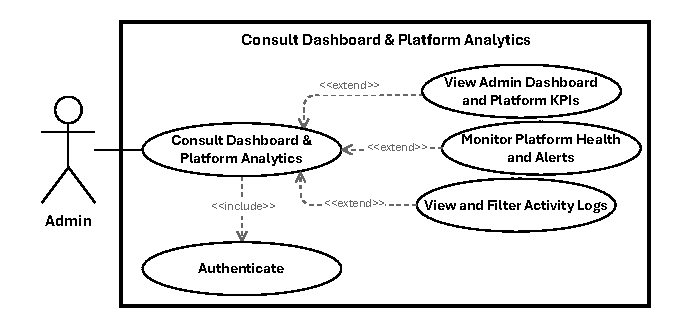
\includegraphics[width=\textwidth]{assets/chapter3/admin-consult-dashboard-and-platform-analytics-use-case}
    \caption{Use Case Consult Dashboard \& Platform Analytics}
    \label{fig:admin-consult-dashboard-and-platform-analytics-use-case}
\end{figure}
\subsubsubsection{Specification of the Use Case View Admin Dashboard and Platform KPIs}
\begin{table}[H]
    \centering
    \caption{Use Case Specification: View Admin Dashboard and Platform KPIs}
    \begin{tabular}{|p{2.7cm}|p{12.5cm}|}
        \hline
        \textbf{Title}          & View Admin Dashboard and Platform KPIs \\
        \hline
        \textbf{Summary}        & Administrator views system-wide key performance indicators including user statistics, revenue, active sessions, and infrastructure health, with the ability to drill down into detailed breakdowns per metric category \\
        \hline
        \textbf{Actor}          & Administrator \\
        \hline
        \textbf{Precondition}   & The administrator is authenticated with admin privileges \\
        \hline
        \textbf{Post-condition} & The administrator has viewed current system KPIs, trend charts, and infrastructure status at the desired level of detail \\
        \hline
        \textbf{Basic Scenario} & \begin{minipage}[t]{\linewidth}
            \begin{enumerate}[topsep=0pt,itemsep=1pt,parsep=0pt,partopsep=0pt]
                \item Administrator opens the admin dashboard; system aggregates and displays real-time KPI cards covering active VM sessions, registered users, pending approvals, revenue, and infrastructure status indicators
                \item Administrator may filter the dashboard by date range or metric category
                \item Administrator drills down into a KPI card to access the detailed platform metrics view, which displays time-series charts and comparative breakdowns across user statistics (total, active, new registrations), revenue data (total, monthly, payout amounts), and session data (active sessions, duration, resource utilization)
                \item Administrator may further filter detailed metrics by date range, user role, or revenue category
            \end{enumerate}
        \end{minipage} \\
        \hline
        \textbf{Error Scenario} & \begin{minipage}[t]{\linewidth}
            \begin{enumerate}[topsep=0pt,itemsep=1pt,parsep=0pt,partopsep=0pt]
                \item If the metrics or KPI service is unavailable, system displays cached data with a staleness warning
                \item If no data exists for the selected period, system shows an empty state message
            \end{enumerate}
        \end{minipage} \\
        \hline
    \end{tabular}
    \label{tab:admin-dashboard-kpis}
\end{table}
\subsubsubsection{Specification of the Use Case Monitor Platform Health and Alerts}
\begin{table}[H]
    \centering
    \caption{Use Case Specification: Monitor Platform Health and Alerts}
    \begin{tabular}{|p{2.7cm}|p{12.5cm}|}
        \hline
        \textbf{Title}          & Monitor Platform Health and Alerts \\
        \hline
        \textbf{Summary}        & Administrator reviews the overall health status of platform services, inspects active system alerts with their severity and context, and acknowledges or resolves alerts to track response actions \\
        \hline
        \textbf{Actor}          & Administrator \\
        \hline
        \textbf{Precondition}   & The administrator is authenticated with admin privileges \\
        \hline
        \textbf{Post-condition} & The administrator has reviewed service health and alert status; any addressed alerts are updated to acknowledged or resolved and recorded accordingly \\
        \hline
        \textbf{Basic Scenario} & \begin{minipage}[t]{\linewidth}
            \begin{enumerate}[topsep=0pt,itemsep=1pt,parsep=0pt,partopsep=0pt]
                \item Administrator navigates to the platform health section; system displays uptime, error rates, and response times for each service (database, cache, queue, external APIs), highlighting any critical or warning conditions
                \item Administrator may drill down into individual service health details and configure health check thresholds and alert rules
                \item Administrator opens the system alerts panel; system displays a prioritized list of active alerts with severity levels; administrator selects an alert to view detailed context including timestamp, severity, affected resources, and suggested actions; administrator may filter by severity, type, or time range
                \item For \textbf{Acknowledge / Resolve}: administrator selects an active alert, enters resolution notes or action taken, and confirms; system updates the alert status, records the resolution, and removes the alert from the active list; administrator may configure automatic alert resolution rules
            \end{enumerate}
        \end{minipage} \\
        \hline
        \textbf{Error Scenario} & \begin{minipage}[t]{\linewidth}
            \begin{enumerate}[topsep=0pt,itemsep=1pt,parsep=0pt,partopsep=0pt]
                \item If the health monitoring service is unavailable, system displays a connection error with a retry option
                \item If a service is unreachable, system marks it as critical and suggests investigation
                \item If the alerting service is unreachable, system displays a connection error with a retry option
                \item If an alert references a deleted resource, system marks it as stale and suggests dismissal
                \item If an alert has already been resolved, system displays a notice
                \item If a resolution update fails, system preserves the previous state and logs the error
            \end{enumerate}
        \end{minipage} \\
        \hline
    \end{tabular}
    \label{tab:admin-health-alerts}
\end{table}
\subsubsubsection{Specification of the Use Case View and Filter Activity Logs}
\begin{table}[H]
    \centering
    \caption{Use Case Specification: View and Filter Activity Logs}
    \begin{tabular}{|p{2.7cm}|p{12.5cm}|}
        \hline
        \textbf{Title}          & View and Filter Activity Logs \\
        \hline
        \textbf{Summary}        & Administrator views a summary of recent platform activity and browses the full paginated activity log, applying filters by date range, user, event type, or severity to locate specific events, with the option to export results for compliance or auditing \\
        \hline
        \textbf{Actor}          & Administrator \\
        \hline
        \textbf{Precondition}   & The administrator is authenticated with admin privileges and the activity logging system is active \\
        \hline
        \textbf{Post-condition} & The administrator has reviewed recent or filtered activity log entries and optionally exported the results \\
        \hline
        \textbf{Basic Scenario} & \begin{minipage}[t]{\linewidth}
            \begin{enumerate}[topsep=0pt,itemsep=1pt,parsep=0pt,partopsep=0pt]
                \item Administrator navigates to the activity section of the admin dashboard; system displays a summary of recent activity grouped by type (user actions, content updates, system events) with timestamps; administrator may filter by activity type or time range and click any entry for detailed information
                \item Administrator navigates to the full Activity Logs view; system retrieves and displays the most recent log entries with pagination, showing timestamp, user, action, and affected resource per entry
                \item Administrator applies filters (date range, user, event type, severity); system updates the display to match the criteria; administrator may save filter configurations for future use
                \item Administrator exports filtered log entries to CSV or PDF for compliance or auditing purposes
            \end{enumerate}
        \end{minipage} \\
        \hline
        \textbf{Error Scenario} & \begin{minipage}[t]{\linewidth}
            \begin{enumerate}[topsep=0pt,itemsep=1pt,parsep=0pt,partopsep=0pt]
                \item If no entries match the filter criteria, system displays an empty state with a descriptive message
                \item If the filter query is too complex, system suggests simplifying the criteria
                \item If log storage or the activity service is temporarily unavailable, system displays an error notification with a retry option
            \end{enumerate}
        \end{minipage} \\
        \hline
    \end{tabular}
    \label{tab:admin-activity-logs}
\end{table}


\subsubsubsection{View Admin Dashboard (KPI Cards, Health Summary)}
\begin{table}[H]
    \centering
    \caption{Use Case Specification: View Admin Dashboard (KPI Cards, Health Summary)}
    \begin{tabular}{|p{2.7cm}|p{12.5cm}|}
        \hline
        \textbf{Title}          & View Admin Dashboard (KPI Cards, Health Summary)                                                                                      \\
        \hline
        \textbf{Summary}        & Administrator views system-wide key performance indicators including active sessions, user counts, revenue, and infrastructure health \\
        \hline
        \textbf{Actor}          & Administrator                                                                                                                         \\
        \hline
        \textbf{Precondition}   & The administrator is authenticated with admin privileges                                                                              \\
        \hline
        \textbf{Post-condition} & The administrator views the current system KPIs and dashboard metrics                                                                 \\
        \hline
        \textbf{Basic Scenario} & \begin{minipage}[t]{\linewidth}
                                      \begin{enumerate}[topsep=0pt,itemsep=1pt,parsep=0pt,partopsep=0pt]
                                          \item Administrator opens the admin dashboard
                                          \item System aggregates real-time metrics: active VM sessions, registered users,
                                                pending approvals, and revenue
                                          \item System displays KPI cards, trend charts, and infrastructure status indicators
                                          \item Administrator may filter the dashboard by date range or metric category
                                          \item Administrator may drill down into individual KPIs for detailed breakdowns
                                      \end{enumerate}
                                  \end{minipage}                                            \\
        \hline
        \textbf{Error Scenario} & \begin{minipage}[t]{\linewidth}
                                      \begin{enumerate}[topsep=0pt,itemsep=1pt,parsep=0pt,partopsep=0pt]
                                          \item If the metrics service is unavailable, the system displays cached data with a
                                                staleness warning
                                          \item If no data exists for the selected period, the system shows an empty-state
                                                message
                                      \end{enumerate}
                                  \end{minipage}                                            \\
        \hline
    \end{tabular}
    \label{tab:admin-dashboard}
\end{table}
\subsubsubsection{Specification of the Use Case View Platform KPIs (Users, Revenue, Sessions)}
\begin{table}[H]
    \centering
    \caption{Use Case Specification: View Platform KPIs (Users, Revenue, Sessions)}
    \begin{tabular}{|p{2.7cm}|p{12.5cm}|}
        \hline
        \textbf{Title}          & View Platform KPIs (Users, Revenue, Sessions)                                                                       \\
        \hline
        \textbf{Summary}        & Administrator views detailed platform-wide metrics including user statistics, revenue data, and session information \\
        \hline
        \textbf{Actor}          & Administrator                                                                                                       \\
        \hline
        \textbf{Precondition}   & The administrator is authenticated with admin privileges                                                            \\
        \hline
        \textbf{Post-condition} & The administrator views detailed platform KPIs with breakdowns and trends                                           \\
        \hline
        \textbf{Basic Scenario} & \begin{minipage}[t]{\linewidth}
                                      \begin{enumerate}[topsep=0pt,itemsep=1pt,parsep=0pt,partopsep=0pt]
                                          \item Administrator navigates to the platform KPIs section
                                          \item System retrieves user statistics: total users, active users, new registrations
                                          \item System retrieves revenue data: total revenue, monthly revenue, payout amounts
                                          \item System retrieves session data: active sessions, session duration, resource
                                                utilization
                                          \item System displays KPIs with time-series charts and comparative metrics
                                          \item Administrator may filter by date range, user role, or revenue category
                                      \end{enumerate}
                                  \end{minipage}                         \\
        \hline
        \textbf{Error Scenario} & \begin{minipage}[t]{\linewidth}
                                      \begin{enumerate}[topsep=0pt,itemsep=1pt,parsep=0pt,partopsep=0pt]
                                          \item If the KPI service is unavailable, the system displays cached data with a
                                                staleness warning
                                          \item If no data exists for the selected period, the system shows an empty-state
                                                message
                                      \end{enumerate}
                                  \end{minipage}                             \\
        \hline
    \end{tabular}
    \label{tab:admin-platform-kpis}
\end{table}
\subsubsubsection{Specification of the Use Case Check Platform Health}
\begin{table}[H]
    \centering
    \caption{Use Case Specification: Check Platform Health}
    \begin{tabular}{|p{2.7cm}|p{12.5cm}|}
        \hline
        \textbf{Title}          & Check Platform Health                                                                                                                \\
        \hline
        \textbf{Summary}        & Administrator reviews the overall health status of the platform including service availability, error rates, and performance metrics \\
        \hline
        \textbf{Actor}          & Administrator                                                                                                                        \\
        \hline
        \textbf{Precondition}   & The administrator is authenticated with admin privileges                                                                             \\
        \hline
        \textbf{Post-condition} & The administrator views the current platform health status and any critical issues                                                   \\
        \hline
        \textbf{Basic Scenario} & \begin{minipage}[t]{\linewidth}
                                      \begin{enumerate}[topsep=0pt,itemsep=1pt,parsep=0pt,partopsep=0pt]
                                          \item Administrator navigates to the platform health section
                                          \item System retrieves health metrics: service uptime, error rates, response times
                                          \item System displays health status for each service: database, cache, queue,
                                                external APIs
                                          \item System highlights any critical or warning conditions
                                          \item Administrator may drill down into individual service health details
                                          \item Administrator may configure health check thresholds and alert rules
                                      \end{enumerate}
                                  \end{minipage}                                            \\
        \hline
        \textbf{Error Scenario} & \begin{minipage}[t]{\linewidth}
                                      \begin{enumerate}[topsep=0pt,itemsep=1pt,parsep=0pt,partopsep=0pt]
                                          \item If the health monitoring service is unavailable, the system displays a
                                                connection error with retry option
                                          \item If a service is unreachable, the system marks it as critical and suggests
                                                investigation
                                      \end{enumerate}
                                  \end{minipage}                                               \\
        \hline
    \end{tabular}
    \label{tab:admin-platform-health}
\end{table}
\subsubsubsection{Specification of the Use Case View System Alerts}
\begin{table}[H]
    \centering
    \caption{Use Case Specification: View System Alerts}
    \begin{tabular}{|p{2.7cm}|p{12.5cm}|}
        \hline
        \textbf{Title}          & View System Alerts                                                                              \\
        \hline
        \textbf{Summary}        & Administrator reviews system alerts generated by infrastructure monitoring and error thresholds \\
        \hline
        \textbf{Actor}          & Administrator                                                                                   \\
        \hline
        \textbf{Precondition}   & The administrator is authenticated with admin privileges                                        \\
        \hline
        \textbf{Post-condition} & The administrator views the current system alerts with severity levels and context              \\
        \hline
        \textbf{Basic Scenario} & \begin{minipage}[t]{\linewidth}
                                      \begin{enumerate}[topsep=0pt,itemsep=1pt,parsep=0pt,partopsep=0pt]
                                          \item Administrator opens the system alerts panel
                                          \item System displays a prioritized list of active alerts with severity levels
                                          \item Administrator selects an alert to view detailed context and affected resources
                                          \item System displays alert details: timestamp, severity, affected resources,
                                                suggested actions
                                          \item Administrator may filter alerts by severity, type, or time range
                                      \end{enumerate}
                                  \end{minipage}     \\
        \hline
        \textbf{Error Scenario} & \begin{minipage}[t]{\linewidth}
                                      \begin{enumerate}[topsep=0pt,itemsep=1pt,parsep=0pt,partopsep=0pt]
                                          \item If the alerting service is unreachable, the system displays a connection error
                                                with retry option
                                          \item If an alert references a deleted resource, the system marks it as stale and
                                                suggests dismissal
                                      \end{enumerate}
                                  \end{minipage}     \\
        \hline
    \end{tabular}
    \label{tab:admin-system-alerts}
\end{table}
\subsubsubsection{Specification of the Use Case Acknowledge / Resolve Alert}
\begin{table}[H]
    \centering
    \caption{Use Case Specification: Acknowledge / Resolve Alert}
    \begin{tabular}{|p{2.7cm}|p{12.5cm}|}
        \hline
        \textbf{Title}          & Acknowledge / Resolve Alert                                                                                  \\
        \hline
        \textbf{Summary}        & Administrator acknowledges or resolves system alerts to track response actions and clear alert notifications \\
        \hline
        \textbf{Actor}          & Administrator                                                                                                \\
        \hline
        \textbf{Precondition}   & The administrator is authenticated with admin privileges and there are active alerts to address              \\
        \hline
        \textbf{Post-condition} & The alert status is updated to acknowledged or resolved and the resolution is recorded                       \\
        \hline
        \textbf{Basic Scenario} & \begin{minipage}[t]{\linewidth}
                                      \begin{enumerate}[topsep=0pt,itemsep=1pt,parsep=0pt,partopsep=0pt]
                                          \item Administrator opens the system alerts panel
                                          \item Administrator selects an alert to acknowledge or resolve
                                          \item Administrator enters resolution notes or action taken
                                          \item System updates the alert status and records the resolution
                                          \item System removes the alert from the active alerts list
                                          \item Administrator may configure automatic alert resolution rules
                                      \end{enumerate}
                                  \end{minipage}                                    \\
        \hline
        \textbf{Error Scenario} & \begin{minipage}[t]{\linewidth}
                                      \begin{enumerate}[topsep=0pt,itemsep=1pt,parsep=0pt,partopsep=0pt]
                                          \item If the alert has already been resolved, the system displays a notice
                                          \item If the resolution update fails, the system preserves the previous state and
                                                logs the error
                                      \end{enumerate}
                                  \end{minipage}                     \\
        \hline
    \end{tabular}
    \label{tab:admin-acknowledge-alert}
\end{table}
\subsubsubsection{Specification of the Use Case View Activity Logs}
\begin{table}[H]
    \centering
    \caption{Use Case Specification: View Activity Logs}
    \begin{tabular}{|p{2.7cm}|p{12.5cm}|}
        \hline
        \textbf{Title}          & View Activity Logs                                                                                                                              \\ \hline
        \textbf{Summary}        & Administrator views a paginated, filterable log of all platform activities including user actions, system events, and administrative operations \\ \hline
        \textbf{Actor}          & Administrator                                                                                                                                   \\ \hline
        \textbf{Precondition}   & The administrator is authenticated with admin privileges; the activity logging system is active                                                 \\ \hline
        \textbf{Post-condition} & The administrator has reviewed the activity log entries matching the applied filters                                                            \\ \hline
        \textbf{Basic Scenario} & \begin{minipage}[t]{\linewidth}
                                      \begin{enumerate}[topsep=0pt,itemsep=1pt,parsep=0pt,partopsep=0pt]
                                          \item Administrator navigates to the Activity Logs section in the admin dashboard
                                          \item System retrieves and displays the most recent activity log entries with
                                                pagination
                                          \item Administrator applies filters by date range, user, event type, or severity
                                                level
                                          \item System updates the log display to match the filter criteria
                                          \item Administrator reviews individual log entries with details including timestamp,
                                                user, action, and affected resource
                                          \item Administrator can export filtered log entries for compliance or auditing
                                                purposes
                                      \end{enumerate}
                                  \end{minipage}                                                     \\ \hline
        \textbf{Error Scenario} & \begin{minipage}[t]{\linewidth}
                                      \begin{enumerate}[topsep=0pt,itemsep=1pt,parsep=0pt,partopsep=0pt]
                                          \item If no log entries match the filter criteria, the system displays an empty state
                                                with a descriptive message
                                          \item If the log storage is temporarily unavailable, the system displays an error
                                                notification and suggests retrying
                                      \end{enumerate}
                                  \end{minipage}                                                    \\ \hline
    \end{tabular}
    \label{tab:admin-activity-logs}
\end{table}
\subsubsubsection{Specification of the Use Case View Recent Activity}
\begin{table}[H]
    \centering
    \caption{Use Case Specification: View Recent Activity}
    \begin{tabular}{|p{2.7cm}|p{12.5cm}|}
        \hline
        \textbf{Title}          & View Recent Activity                                                                                                                   \\ \hline
        \textbf{Summary}        & Administrator views a summary of recent platform activities including user registrations, training path submissions, and system events \\ \hline
        \textbf{Actor}          & Administrator                                                                                                                          \\ \hline
        \textbf{Precondition}   & The administrator is authenticated with admin privileges; the activity logging system is active                                        \\ \hline
        \textbf{Post-condition} & The administrator views a summary of recent platform activities with timestamps and context                                            \\ \hline
        \textbf{Basic Scenario} & \begin{minipage}[t]{\linewidth}
                                      \begin{enumerate}[topsep=0pt,itemsep=1pt,parsep=0pt,partopsep=0pt]
                                          \item Administrator navigates to the Recent Activity section in the admin dashboard
                                          \item System retrieves and displays the most recent activity entries with pagination
                                          \item System displays activities grouped by type: user actions, content updates,
                                                system events
                                          \item Administrator may filter by activity type or time range
                                          \item Administrator can click on an activity to view detailed information
                                      \end{enumerate}
                                  \end{minipage}                                            \\ \hline
        \textbf{Error Scenario} & \begin{minipage}[t]{\linewidth}
                                      \begin{enumerate}[topsep=0pt,itemsep=1pt,parsep=0pt,partopsep=0pt]
                                          \item If no recent activity exists, the system displays an empty-state message
                                          \item If the activity service is unavailable, the system displays an error
                                                notification
                                      \end{enumerate}
                                  \end{minipage}                                                  \\ \hline
    \end{tabular}
    \label{tab:admin-recent-activity}
\end{table}
\subsubsubsection{Specification of the Use Case Filter Logs}
\begin{table}[H]
    \centering
    \caption{Use Case Specification: Filter Logs}
    \begin{tabular}{|p{2.7cm}|p{12.5cm}|}
        \hline
        \textbf{Title}          & Filter Logs                                                                                          \\ \hline
        \textbf{Summary}        & Administrator applies filters to activity logs to search for specific events, users, or time periods \\ \hline
        \textbf{Actor}          & Administrator                                                                                        \\ \hline
        \textbf{Precondition}   & The administrator is authenticated with admin privileges; the activity logging system is active      \\ \hline
        \textbf{Post-condition} & The administrator views filtered log entries matching the specified criteria                         \\ \hline
        \textbf{Basic Scenario} & \begin{minipage}[t]{\linewidth}
                                      \begin{enumerate}[topsep=0pt,itemsep=1pt,parsep=0pt,partopsep=0pt]
                                          \item Administrator navigates to the Activity Logs section
                                          \item Administrator selects filter criteria: date range, user, event type, severity
                                          \item System applies the filters and retrieves matching log entries
                                          \item System displays filtered results with pagination
                                          \item Administrator may save filter configurations for future use
                                          \item Administrator can export filtered results to CSV or PDF
                                      \end{enumerate}
                                  \end{minipage}           \\ \hline
        \textbf{Error Scenario} & \begin{minipage}[t]{\linewidth}
                                      \begin{enumerate}[topsep=0pt,itemsep=1pt,parsep=0pt,partopsep=0pt]
                                          \item If no log entries match the filter criteria, the system displays an empty-state
                                                message
                                          \item If the filter query is too complex, the system suggests simplifying the
                                                criteria
                                      \end{enumerate}
                                  \end{minipage}         \\ \hline
    \end{tabular}
    \label{tab:admin-filter-logs}
\end{table}


\subsubsection[Refinement of the Use Case Set Maintenance Mode]{Refinement of the Use Case Set Maintenance Mode} Figure
\ref{fig:admin-set-maintenance-mode-use-case} presents the refinement of the
Use Case Set Maintenance Mode for the Administrator actor. This use case includes
the following sub-use cases:
\begin{figure}[H]
    \centering
    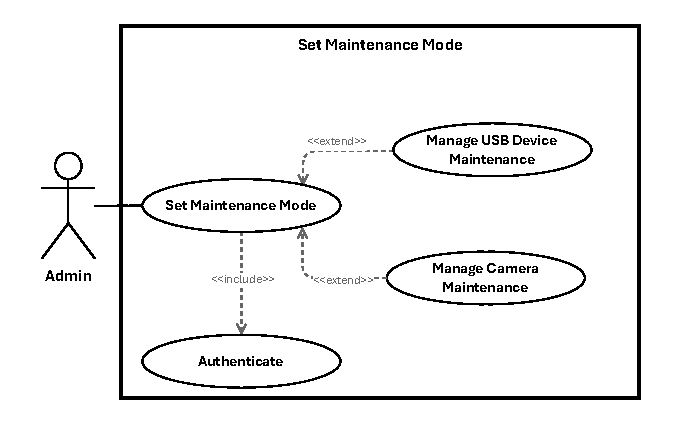
\includegraphics[width=\textwidth]{assets/chapter3/admin-set-maintenance-mode-use-case}
    \caption{Use Case Set Maintenance Mode}
    \label{fig:admin-set-maintenance-mode-use-case}
\end{figure}
\subsubsubsection{Specification of the Use Case Manage USB Device Maintenance}
\begin{table}[H]
    \centering
    \caption{Use Case Specification: Manage USB Device Maintenance}
    \begin{tabular}{|p{2.7cm}|p{12.5cm}|}
        \hline
        \textbf{Title}          & Manage USB Device Maintenance \\
        \hline
        \textbf{Summary}        & Administrator views all USB devices in maintenance, places available devices into maintenance mode with a reason and description, updates maintenance descriptions, and removes devices from maintenance to restore their availability \\
        \hline
        \textbf{Actor}          & Administrator \\
        \hline
        \textbf{Precondition}   & The administrator is authenticated with admin privileges; the target device must be in the appropriate state for the requested action \\
        \hline
        \textbf{Post-condition} & The USB device maintenance status and description are updated accordingly; devices in maintenance cannot accept new reservations and devices removed from maintenance become available again \\
        \hline
        \textbf{Basic Scenario} & \begin{minipage}[t]{\linewidth}
            \begin{enumerate}[topsep=0pt,itemsep=1pt,parsep=0pt,partopsep=0pt]
                \item Administrator navigates to the Maintenance section; system displays all devices currently in maintenance with type, model, maintenance reason, and start date; administrator may filter by device type or reason
                \item For \textbf{Enable}: administrator selects an available USB device and clicks Enable Maintenance; system displays a form for the maintenance reason and description; administrator submits; system updates the device status to maintenance, prevents new reservations, and confirms the activation
                \item For \textbf{Update Description}: administrator selects a device already in maintenance and clicks Edit Maintenance Description; administrator enters or updates the description; system saves the update and confirms
                \item For \textbf{Disable}: administrator selects a device in maintenance and clicks Disable Maintenance; system confirms the action, updates the device status to available, clears the maintenance description, and confirms the deactivation
            \end{enumerate}
        \end{minipage} \\
        \hline
        \textbf{Error Scenario} & \begin{minipage}[t]{\linewidth}
            \begin{enumerate}[topsep=0pt,itemsep=1pt,parsep=0pt,partopsep=0pt]
                \item If no devices are in maintenance, system displays an empty state
                \item If the device list cannot be retrieved, system shows an error notification
                \item If the device is already in the target maintenance state, system displays an explanatory notice
                \item If a description update is attempted on a device not in maintenance, system displays an error
                \item Persistence failures for any action retain the current state and surface a recoverable error
            \end{enumerate}
        \end{minipage} \\
        \hline
    \end{tabular}
    \label{tab:admin-usb-maintenance}
\end{table}
\subsubsubsection{Specification of the Use Case Set VM Maintenance Mode}
\begin{table}[H]
    \centering
    \caption{Use Case Specification: Set VM Maintenance Mode}
    \begin{tabular}{|p{2.7cm}|p{12.5cm}|}
        \hline
        \textbf{Title}          & Set VM Maintenance Mode \\
        \hline
        \textbf{Summary}        & Administrator enables or disables maintenance mode on Proxmox nodes hosting VMs to perform infrastructure updates safely \\
        \hline
        \textbf{Actor}          & Administrator \\
        \hline
        \textbf{Precondition}   & The administrator is authenticated with admin privileges \\
        \hline
        \textbf{Post-condition} & The target node's maintenance mode status is updated and active VM sessions are handled per policy \\
        \hline
        \textbf{Basic Scenario} & \begin{minipage}[t]{\linewidth}
                                      \begin{enumerate}[topsep=0pt,itemsep=1pt,parsep=0pt,partopsep=0pt]
                                          \item Administrator selects a Proxmox node from the infrastructure panel
                                          \item System displays the node's current status, active VMs, and resource utilization
                                          \item Administrator enables maintenance mode on the node
                                          \item System prevents new VM provisioning on the node and notifies affected users
                                          \item System gracefully migrates or terminates active sessions per configured policy
                                          \item Administrator performs the maintenance and disables maintenance mode when complete
                                          \item System restores the node to available status and resumes normal provisioning
                                      \end{enumerate}
                                  \end{minipage} \\
        \hline
        \textbf{Error Scenario} & \begin{minipage}[t]{\linewidth}
                                      \begin{enumerate}[topsep=0pt,itemsep=1pt,parsep=0pt,partopsep=0pt]
                                          \item If live migration fails for an active VM, the system alerts the administrator and offers a force-stop option
                                          \item If the node becomes unresponsive during maintenance, the system marks it as offline and escalates the alert
                                      \end{enumerate}
                                  \end{minipage} \\
        \hline
    \end{tabular}
    \label{tab:admin-vm-maintenance-mode}
\end{table}
\subsubsubsection{Specification of the Use Case Manage Camera Maintenance}
\begin{table}[H]
    \centering
    \caption{Use Case Specification: Manage Camera Maintenance}
    \begin{tabular}{|p{2.7cm}|p{12.5cm}|}
        \hline
        \textbf{Title}          & Manage Camera Maintenance \\
        \hline
        \textbf{Summary}        & Administrator places cameras into maintenance mode to prevent streaming and assignment, and removes them from maintenance to restore availability \\
        \hline
        \textbf{Actor}          & Administrator \\
        \hline
        \textbf{Precondition}   & The administrator is authenticated with admin privileges; the target camera must be in the appropriate state for the requested action \\
        \hline
        \textbf{Post-condition} & The camera maintenance status is updated; cameras in maintenance cannot be streamed or assigned, and cameras removed from maintenance become available again \\
        \hline
        \textbf{Basic Scenario} & \begin{minipage}[t]{\linewidth}
            \begin{enumerate}[topsep=0pt,itemsep=1pt,parsep=0pt,partopsep=0pt]
                \item Administrator selects a camera from the device list and chooses a maintenance action
                \item For \textbf{Enable}: administrator clicks Enable Maintenance; system displays a form for the maintenance reason and description; administrator submits; system updates the camera status to maintenance, prevents streaming and assignment, and confirms the activation
                \item For \textbf{Disable}: administrator selects a camera in maintenance and clicks Disable Maintenance; system confirms the action, updates the camera status to available, clears the maintenance description, and confirms the deactivation
            \end{enumerate}
        \end{minipage} \\
        \hline
        \textbf{Error Scenario} & \begin{minipage}[t]{\linewidth}
            \begin{enumerate}[topsep=0pt,itemsep=1pt,parsep=0pt,partopsep=0pt]
                \item If the camera is already in the target maintenance state, system displays an explanatory notice
                \item Persistence failures for any action retain the current state and surface a recoverable error
            \end{enumerate}
        \end{minipage} \\
        \hline
    \end{tabular}
    \label{tab:admin-camera-maintenance}
\end{table}


\subsubsubsection{Specification of the Use Case View All Devices in Maintenance}
\begin{table}[H]
    \centering
    \caption{Use Case Specification: View All Devices in Maintenance}
    \begin{tabular}{|p{2.7cm}|p{12.5cm}|}
        \hline
        \textbf{Title}          & View All Devices in Maintenance                                                             \\
        \hline
        \textbf{Summary}        & Administrator views all hardware devices currently in maintenance mode                      \\
        \hline
        \textbf{Actor}          & Administrator                                                                               \\
        \hline
        \textbf{Precondition}   & The administrator is authenticated with admin privileges                                    \\
        \hline
        \textbf{Post-condition} & The administrator views a list of devices in maintenance with their maintenance details     \\
        \hline
        \textbf{Basic Scenario} & \begin{minipage}[t]{\linewidth}
                                      \begin{enumerate}[topsep=0pt,itemsep=1pt,parsep=0pt,partopsep=0pt]
                                          \item Administrator navigates to the Maintenance section
                                          \item System retrieves all devices in maintenance mode
                                          \item System displays devices with type, model, maintenance reason, and start date
                                          \item Administrator can filter devices by type or maintenance reason
                                          \item Administrator can view detailed maintenance information
                                      \end{enumerate}
                                  \end{minipage}   \\
        \hline
        \textbf{Error Scenario} & \begin{minipage}[t]{\linewidth}
                                      \begin{enumerate}[topsep=0pt,itemsep=1pt,parsep=0pt,partopsep=0pt]
                                          \item If no devices are in maintenance, the system displays an empty-state message
                                          \item If the device list cannot be retrieved, the system shows an error notification
                                      \end{enumerate}
                                  \end{minipage} \\
        \hline
    \end{tabular}
    \label{tab:admin-view-maintenance-devices}
\end{table}
\subsubsubsection{Specification of the Use Case Set USB Device Maintenance Description}
\begin{table}[H]
    \centering
    \caption{Use Case Specification: Set USB Device Maintenance Description}
    \begin{tabular}{|p{2.7cm}|p{12.5cm}|}
        \hline
        \textbf{Title}          & Set USB Device Maintenance Description                                                 \\
        \hline
        \textbf{Summary}        & Administrator adds or updates the maintenance description for a USB device             \\
        \hline
        \textbf{Actor}          & Administrator                                                                          \\
        \hline
        \textbf{Precondition}   & The administrator is authenticated and has selected a USB device in maintenance        \\
        \hline
        \textbf{Post-condition} & The USB device maintenance description is updated and visible to users                 \\
        \hline
        \textbf{Basic Scenario} & \begin{minipage}[t]{\linewidth}
                                      \begin{enumerate}[topsep=0pt,itemsep=1pt,parsep=0pt,partopsep=0pt]
                                          \item Administrator selects a USB device in maintenance
                                          \item Administrator clicks Edit Maintenance Description
                                          \item System displays the maintenance description form
                                          \item Administrator enters or updates the maintenance description
                                          \item System saves the description and updates the device record
                                          \item System confirms the update and displays the new description
                                      \end{enumerate}
                                  \end{minipage}               \\
        \hline
        \textbf{Error Scenario} & \begin{minipage}[t]{\linewidth}
                                      \begin{enumerate}[topsep=0pt,itemsep=1pt,parsep=0pt,partopsep=0pt]
                                          \item If the device is not in maintenance, the system displays an error
                                          \item If the update fails, the system displays an error and retains the current
                                                description
                                      \end{enumerate}
                                  \end{minipage} \\
        \hline
    \end{tabular}
    \label{tab:admin-set-usb-maintenance-description}
\end{table}
\subsubsubsection{Specification of the Use Case Enable USB Device Maintenance}
\begin{table}[H]
    \centering
    \caption{Use Case Specification: Enable USB Device Maintenance}
    \begin{tabular}{|p{2.7cm}|p{12.5cm}|}
        \hline
        \textbf{Title}          & Enable USB Device Maintenance                                                              \\
        \hline
        \textbf{Summary}        & Administrator places a USB device into maintenance mode to prevent new reservations        \\
        \hline
        \textbf{Actor}          & Administrator                                                                              \\
        \hline
        \textbf{Precondition}   & The administrator is authenticated and has selected an available USB device                \\
        \hline
        \textbf{Post-condition} & The USB device is placed in maintenance mode and no new reservations can be made           \\
        \hline
        \textbf{Basic Scenario} & \begin{minipage}[t]{\linewidth}
                                      \begin{enumerate}[topsep=0pt,itemsep=1pt,parsep=0pt,partopsep=0pt]
                                          \item Administrator selects an available USB device
                                          \item Administrator clicks Enable Maintenance
                                          \item System displays the maintenance form with description field
                                          \item Administrator enters the maintenance reason and description
                                          \item System updates the device status to maintenance
                                          \item System prevents new reservations for the device
                                          \item System confirms the maintenance mode activation
                                      \end{enumerate}
                                  \end{minipage}                   \\
        \hline
        \textbf{Error Scenario} & \begin{minipage}[t]{\linewidth}
                                      \begin{enumerate}[topsep=0pt,itemsep=1pt,parsep=0pt,partopsep=0pt]
                                          \item If the device is already in maintenance, the system displays a notice
                                          \item If the maintenance activation fails, the system displays an error and retains
                                                the current state
                                      \end{enumerate}
                                  \end{minipage} \\
        \hline
    \end{tabular}
    \label{tab:admin-enable-usb-maintenance}
\end{table}
\subsubsubsection{Specification of the Use Case Disable USB Device Maintenance}
\begin{table}[H]
    \centering
    \caption{Use Case Specification: Disable USB Device Maintenance}
    \begin{tabular}{|p{2.7cm}|p{12.5cm}|}
        \hline
        \textbf{Title}          & Disable USB Device Maintenance                                                                 \\
        \hline
        \textbf{Summary}        & Administrator removes a USB device from maintenance mode, making it available for reservations \\
        \hline
        \textbf{Actor}          & Administrator                                                                                  \\
        \hline
        \textbf{Precondition}   & The administrator is authenticated and has selected a USB device in maintenance                \\
        \hline
        \textbf{Post-condition} & The USB device is removed from maintenance mode and becomes available for reservations         \\
        \hline
        \textbf{Basic Scenario} & \begin{minipage}[t]{\linewidth}
                                      \begin{enumerate}[topsep=0pt,itemsep=1pt,parsep=0pt,partopsep=0pt]
                                          \item Administrator selects a USB device in maintenance
                                          \item Administrator clicks Disable Maintenance
                                          \item System confirms the action
                                          \item System updates the device status to available
                                          \item System clears the maintenance description
                                          \item System confirms the maintenance mode deactivation
                                      \end{enumerate}
                                  \end{minipage}                          \\
        \hline
        \textbf{Error Scenario} & \begin{minipage}[t]{\linewidth}
                                      \begin{enumerate}[topsep=0pt,itemsep=1pt,parsep=0pt,partopsep=0pt]
                                          \item If the device is not in maintenance, the system displays a notice
                                          \item If the maintenance deactivation fails, the system displays an error and retains
                                                the current state
                                      \end{enumerate}
                                  \end{minipage}   \\
        \hline
    \end{tabular}
    \label{tab:admin-disable-usb-maintenance}
\end{table}
\subsubsubsection{Specification of the Use Case Enable Camera Maintenance Mode}
\begin{table}[H]
    \centering
    \caption{Use Case Specification: Enable Camera Maintenance Mode}
    \begin{tabular}{|p{2.7cm}|p{12.5cm}|}
        \hline
        \textbf{Title}          & Enable Camera Maintenance Mode                                                             \\
        \hline
        \textbf{Summary}        & Administrator places a camera into maintenance mode to prevent streaming and assignment    \\
        \hline
        \textbf{Actor}          & Administrator                                                                              \\
        \hline
        \textbf{Precondition}   & The administrator is authenticated and has selected an available camera                    \\
        \hline
        \textbf{Post-condition} & The camera is placed in maintenance mode and no streaming or assignment can occur          \\
        \hline
        \textbf{Basic Scenario} & \begin{minipage}[t]{\linewidth}
                                      \begin{enumerate}[topsep=0pt,itemsep=1pt,parsep=0pt,partopsep=0pt]
                                          \item Administrator selects an available camera
                                          \item Administrator clicks Enable Maintenance
                                          \item System displays the maintenance form with description field
                                          \item Administrator enters the maintenance reason and description
                                          \item System updates the camera status to maintenance
                                          \item System prevents streaming and assignment for the camera
                                          \item System confirms the maintenance mode activation
                                      \end{enumerate}
                                  \end{minipage}                   \\
        \hline
        \textbf{Error Scenario} & \begin{minipage}[t]{\linewidth}
                                      \begin{enumerate}[topsep=0pt,itemsep=1pt,parsep=0pt,partopsep=0pt]
                                          \item If the camera is already in maintenance, the system displays a notice
                                          \item If the maintenance activation fails, the system displays an error and retains
                                                the current state
                                      \end{enumerate}
                                  \end{minipage} \\
        \hline
    \end{tabular}
    \label{tab:admin-enable-camera-maintenance}
\end{table}
\subsubsubsection{Specification of the Use Case Disable Camera Maintenance Mode}
\begin{table}[H]
    \centering
    \caption{Use Case Specification: Disable Camera Maintenance Mode}
    \begin{tabular}{|p{2.7cm}|p{12.5cm}|}
        \hline
        \textbf{Title}          & Disable Camera Maintenance Mode                                                                        \\
        \hline
        \textbf{Summary}        & Administrator removes a camera from maintenance mode, making it available for streaming and assignment \\
        \hline
        \textbf{Actor}          & Administrator                                                                                          \\
        \hline
        \textbf{Precondition}   & The administrator is authenticated and has selected a camera in maintenance                            \\
        \hline
        \textbf{Post-condition} & The camera is removed from maintenance mode and becomes available for streaming and assignment         \\
        \hline
        \textbf{Basic Scenario} & \begin{minipage}[t]{\linewidth}
                                      \begin{enumerate}[topsep=0pt,itemsep=1pt,parsep=0pt,partopsep=0pt]
                                          \item Administrator selects a camera in maintenance
                                          \item Administrator clicks Disable Maintenance
                                          \item System confirms the action
                                          \item System updates the camera status to available
                                          \item System clears the maintenance description
                                          \item System confirms the maintenance mode deactivation
                                      \end{enumerate}
                                  \end{minipage}                                  \\
        \hline
        \textbf{Error Scenario} & \begin{minipage}[t]{\linewidth}
                                      \begin{enumerate}[topsep=0pt,itemsep=1pt,parsep=0pt,partopsep=0pt]
                                          \item If the camera is not in maintenance, the system displays a notice
                                          \item If the maintenance deactivation fails, the system displays an error and retains
                                                the current state
                                      \end{enumerate}
                                  \end{minipage}           \\
        \hline
    \end{tabular}
    \label{tab:admin-disable-camera-maintenance}
\end{table}



\subsubsubsection{Specification of the Use Case Moderate Forum Threads}
\begin{table}[H]
    \centering
    \caption{Use Case Specification: Moderate Forum Threads}
    \begin{tabular}{|p{2.7cm}|p{12.5cm}|}
        \hline
        \textbf{Title}          & Moderate Forum Threads \\
        \hline
        \textbf{Summary}        & Administrator reviews flagged forum threads and replies reported by users, and dismisses flags on content that does not warrant removal, restoring it to normal status \\
        \hline
        \textbf{Actor}          & Administrator \\
        \hline
        \textbf{Precondition}   & The administrator is authenticated with admin privileges \\
        \hline
        \textbf{Post-condition} & Reviewed content is either unflagged and removed from the moderation queue, or retained pending further action; all moderation decisions are logged for audit purposes \\
        \hline
        \textbf{Basic Scenario} & \begin{minipage}[t]{\linewidth}
            \begin{enumerate}[topsep=0pt,itemsep=1pt,parsep=0pt,partopsep=0pt]
                \item Administrator navigates to the Forum Moderation section; system displays a prioritized list of flagged threads and replies with flag reason, reporter, and post content; administrator may filter by severity, type, or time range
                \item Administrator selects a flagged item and reviews its full thread context and flag reason
                \item If the content does not warrant action, administrator selects Unflag; system removes the flag from the thread or reply, clears it from the moderation queue, and logs the decision for audit purposes
            \end{enumerate}
        \end{minipage} \\
        \hline
        \textbf{Error Scenario} & \begin{minipage}[t]{\linewidth}
            \begin{enumerate}[topsep=0pt,itemsep=1pt,parsep=0pt,partopsep=0pt]
                \item If no flagged posts exist, system displays an empty state
                \item If the forum service is unavailable, system displays an error notification
                \item If the selected item has already been unflagged, system displays an explanatory notice
                \item If the unflag action fails, system retains the current flag state and surfaces a recoverable error
            \end{enumerate}
        \end{minipage} \\
        \hline
    \end{tabular}
    \label{tab:admin-moderate-forum}
\end{table}


\subsubsection[Refinement of the Use Case Moderate Forum Threads]{Refinement of the Use Case Moderate Forum Threads} Figure
\ref{fig:admin-consult-dashboard-and-platform-analytics-use-case} presents the refinement of the
Use Case Moderate Forum Threads for the Administrator actor. This use case includes
the following sub-use cases:
\begin{figure}[H]
    \centering
    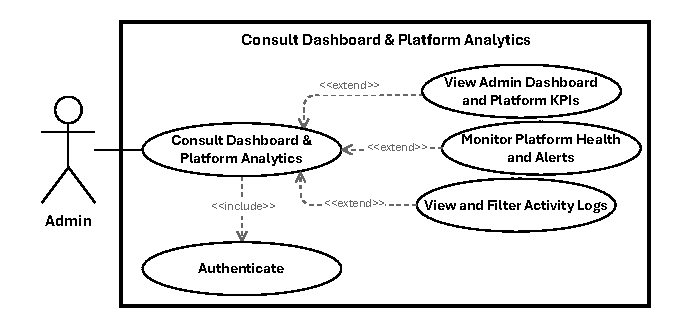
\includegraphics[width=\textwidth]{assets/chapter3/admin-consult-dashboard-and-platform-analytics-use-case}
    \caption{Use Case Moderate Forum Threads}
    \label{fig:admin-consult-dashboard-and-platform-analytics-use-case}
\end{figure}
\subsubsubsection{Specification of the Use Case View Flagged Threads \& Replies}
\begin{table}[H]
    \centering
    \caption{Use Case Specification: View Flagged Threads \& Replies}
    \begin{tabular}{|p{2.7cm}|p{12.5cm}|}
        \hline
        \textbf{Title}          & View Flagged Threads \& Replies                                                                        \\ \hline
        \textbf{Summary}        & Administrator views a list of flagged forum threads and replies that have been reported by users       \\ \hline
        \textbf{Actor}          & Administrator                                                                                          \\ \hline
        \textbf{Precondition}   & The administrator is authenticated with admin privileges; there are flagged forum posts pending review \\ \hline
        \textbf{Post-condition} & The administrator views the list of flagged posts with details and can take moderation actions         \\ \hline
        \textbf{Basic Scenario} & \begin{minipage}[t]{\linewidth}
                                      \begin{enumerate}[topsep=0pt,itemsep=1pt,parsep=0pt,partopsep=0pt]
                                          \item Administrator navigates to the Forum Moderation section
                                          \item System displays a list of flagged forum posts with flag reason, reporter, and
                                                post content
                                          \item Administrator can filter flagged posts by severity, type, or time range
                                          \item Administrator can view the full thread context for each flagged post
                                          \item Administrator can select a post to take moderation action
                                      \end{enumerate}
                                  \end{minipage}             \\ \hline
        \textbf{Error Scenario} & \begin{minipage}[t]{\linewidth}
                                      \begin{enumerate}[topsep=0pt,itemsep=1pt,parsep=0pt,partopsep=0pt]
                                          \item If no flagged posts exist, the system displays an empty-state message
                                          \item If the forum service is unavailable, the system displays an error notification
                                      \end{enumerate}
                                  \end{minipage}            \\ \hline
    \end{tabular}
    \label{tab:admin-view-flagged}
\end{table}
\subsubsubsection{Specification of the Use Case Unflag Thread}
\begin{table}[H]
    \centering
    \caption{Use Case Specification: Unflag Thread}
    \begin{tabular}{|p{2.7cm}|p{12.5cm}|}
        \hline
        \textbf{Title}          & Unflag Thread                                                                                                       \\ \hline
        \textbf{Summary}        & Administrator removes the flag from a forum thread, dismissing the report and restoring the thread to normal status \\ \hline
        \textbf{Actor}          & Administrator                                                                                                       \\ \hline
        \textbf{Precondition}   & The administrator is authenticated with admin privileges and there is a flagged thread to unflag                    \\ \hline
        \textbf{Post-condition} & The thread flag is removed and the thread is no longer in the moderation queue                                      \\ \hline
        \textbf{Basic Scenario} & \begin{minipage}[t]{\linewidth}
                                      \begin{enumerate}[topsep=0pt,itemsep=1pt,parsep=0pt,partopsep=0pt]
                                          \item Administrator selects a flagged thread from the moderation queue
                                          \item Administrator reviews the thread content and flag reason
                                          \item Administrator selects the unflag action
                                          \item System removes the flag from the thread
                                          \item System removes the thread from the moderation queue
                                          \item System logs the unflag action for audit purposes
                                      \end{enumerate}
                                  \end{minipage}                                       \\ \hline
        \textbf{Error Scenario} & \begin{minipage}[t]{\linewidth}
                                      \begin{enumerate}[topsep=0pt,itemsep=1pt,parsep=0pt,partopsep=0pt]
                                          \item If the thread has already been unflagged, the system displays a notice
                                          \item If the unflag action fails, the system displays an error and retains the
                                                current state
                                      \end{enumerate}
                                  \end{minipage}                               \\ \hline
    \end{tabular}
    \label{tab:admin-unflag-thread}
\end{table}
\subsubsubsection{Specification of the Use Case Unflag Reply}
\begin{table}[H]
    \centering
    \caption{Use Case Specification: Unflag Reply}
    \begin{tabular}{|p{2.7cm}|p{12.5cm}|}
        \hline
        \textbf{Title}          & Unflag Reply                                                                                                      \\ \hline
        \textbf{Summary}        & Administrator removes the flag from a forum reply, dismissing the report and restoring the reply to normal status \\ \hline
        \textbf{Actor}          & Administrator                                                                                                     \\ \hline
        \textbf{Precondition}   & The administrator is authenticated with admin privileges and there is a flagged reply to unflag                   \\ \hline
        \textbf{Post-condition} & The reply flag is removed and the reply is no longer in the moderation queue                                      \\ \hline
        \textbf{Basic Scenario} & \begin{minipage}[t]{\linewidth}
                                      \begin{enumerate}[topsep=0pt,itemsep=1pt,parsep=0pt,partopsep=0pt]
                                          \item Administrator selects a flagged reply from the moderation queue
                                          \item Administrator reviews the reply content and flag reason
                                          \item Administrator selects the unflag action
                                          \item System removes the flag from the reply
                                          \item System removes the reply from the moderation queue
                                          \item System logs the unflag action for audit purposes
                                      \end{enumerate}
                                  \end{minipage}                                      \\ \hline
        \textbf{Error Scenario} & \begin{minipage}[t]{\linewidth}
                                      \begin{enumerate}[topsep=0pt,itemsep=1pt,parsep=0pt,partopsep=0pt]
                                          \item If the reply has already been unflagged, the system displays a notice
                                          \item If the unflag action fails, the system displays an error and retains the
                                                current state
                                      \end{enumerate}
                                  \end{minipage}                             \\ \hline
    \end{tabular}
    \label{tab:admin-unflag-reply}
\end{table}


\subsubsection[Refinement of the Use Case Manage Training Paths]{Refinement of the Use Case Manage Training Paths} Figure
\ref{fig:admin-manage-training-paths-use-case} presents the refinement of the
Use Case Manage Training Paths for the Administrator actor. This use case includes
the following sub-use cases:
\begin{figure}[H]
    \centering
    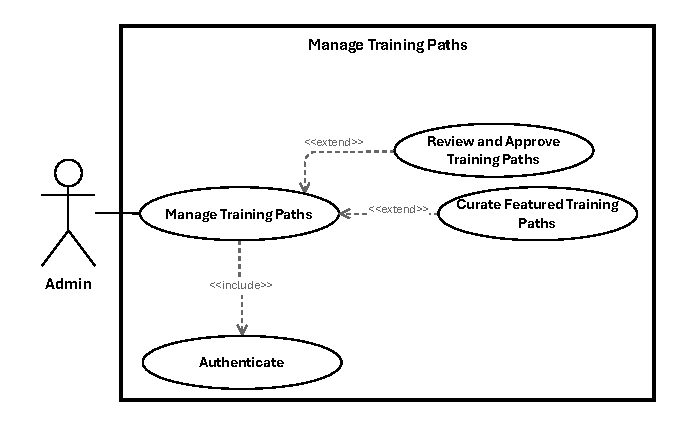
\includegraphics[width=\textwidth]{assets/chapter3/admin-manage-training-paths-use-case}
    \caption{Use Case Manage Training Paths}
    \label{fig:admin-manage-training-paths-use-case}
\end{figure}
\subsubsubsection{Specification of the Use Case Review and Approve Training Paths}
\begin{table}[H]
    \centering
    \caption{Use Case Specification: Review and Approve Training Paths}
    \begin{tabular}{|p{2.7cm}|p{12.5cm}|}
        \hline
        \textbf{Title}          & Review and Approve Training Paths \\
        \hline
        \textbf{Summary}        & Administrator browses all training paths, reviews submitted ones pending approval, and approves or rejects them with feedback to control what is published on the platform \\
        \hline
        \textbf{Actor}          & Administrator \\
        \hline
        \textbf{Precondition}   & The administrator is authenticated and authorized through the admin-only policy; at least one training path exists or is pending review \\
        \hline
        \textbf{Post-condition} & The training path status is updated to approved or rejected; approved paths become available in public listings and the author is notified in either case \\
        \hline
        \textbf{Basic Scenario} & \begin{minipage}[t]{\linewidth}
            \begin{enumerate}[topsep=0pt,itemsep=1pt,parsep=0pt,partopsep=0pt]
                \item Administrator navigates to the Training Paths section; system displays all training paths with title, author, status, and approval state; administrator may filter by status or approval state
                \item Administrator selects a path pending review and inspects its pedagogical and operational information
                \item For \textbf{Approve}: administrator confirms the approval; system updates the training path status to approved, makes it available within public listings, and notifies the author
                \item For \textbf{Reject}: administrator clicks Reject and enters feedback explaining the reasons; system updates the status to rejected, sends the feedback to the author as a notification, and retains the path for revision
            \end{enumerate}
        \end{minipage} \\
        \hline
        \textbf{Error Scenario} & \begin{minipage}[t]{\linewidth}
            \begin{enumerate}[topsep=0pt,itemsep=1pt,parsep=0pt,partopsep=0pt]
                \item If no training paths exist or the list cannot be retrieved, system displays an appropriate empty state or error notification
                \item If the training path no longer satisfies review conditions, approval is refused
                \item If the path is already approved or rejected, system displays an explanatory notice
                \item If the administrator lacks permission, the action is denied
                \item Persistence failures for any action retain the previous state and log the failure
            \end{enumerate}
        \end{minipage} \\
        \hline
    \end{tabular}
    \label{tab:admin-review-training-paths}
\end{table}
\subsubsubsection{Specification of the Use Case Curate Featured Training Paths}
\begin{table}[H]
    \centering
    \caption{Use Case Specification: Curate Featured Training Paths}
    \begin{tabular}{|p{2.7cm}|p{12.5cm}|}
        \hline
        \textbf{Title}          & Curate Featured Training Paths \\
        \hline
        \textbf{Summary}        & Administrator marks approved training paths as featured or removes their featured status, and reorders featured paths to control their display sequence on the landing page \\
        \hline
        \textbf{Actor}          & Administrator \\
        \hline
        \textbf{Precondition}   & The administrator is authenticated with admin privileges and the target training path is approved \\
        \hline
        \textbf{Post-condition} & The training path featured status is updated and the landing page reflects the new selection and order \\
        \hline
        \textbf{Basic Scenario} & \begin{minipage}[t]{\linewidth}
            \begin{enumerate}[topsep=0pt,itemsep=1pt,parsep=0pt,partopsep=0pt]
                \item For \textbf{Feature / Unfeature}: administrator selects an approved training path and clicks Feature or Unfeature; system updates the featured status and confirms; the path appears in or disappears from featured listings accordingly
                \item For \textbf{Reorder}: administrator navigates to the Featured Paths section; system displays all featured paths with their current display order; administrator drags and drops paths to the desired sequence; system updates order values for all featured paths and confirms
            \end{enumerate}
        \end{minipage} \\
        \hline
        \textbf{Error Scenario} & \begin{minipage}[t]{\linewidth}
            \begin{enumerate}[topsep=0pt,itemsep=1pt,parsep=0pt,partopsep=0pt]
                \item If the training path is not approved, featuring is blocked with an explanatory error
                \item If fewer than two featured paths exist, reordering displays an explanatory notice
                \item Persistence failures for any action retain the current state and surface a recoverable error
            \end{enumerate}
        \end{minipage} \\
        \hline
    \end{tabular}
    \label{tab:admin-curate-featured}
\end{table}


\subsubsubsection{Specification of the Use Case Manage VM Assignment Queue}
\begin{table}[H]
    \centering
    \caption{Use Case Specification: Manage VM Assignment Queue}
    \begin{tabular}{|p{2.7cm}|p{12.5cm}|}
        \hline
        \textbf{Title}          & Manage VM Assignment Queue \\
        \hline
        \textbf{Summary}        & Administrator browses pending VM assignment requests submitted by teachers, inspects their details and resource requirements, and approves or rejects them with feedback \\
        \hline
        \textbf{Actor}          & Administrator \\
        \hline
        \textbf{Precondition}   & The administrator is authenticated with admin privileges \\
        \hline
        \textbf{Post-condition} & The VM assignment request status is updated to approved or rejected; the VM template is linked to the training unit on approval, and the teacher is notified in either case \\
        \hline
        \textbf{Basic Scenario} & \begin{minipage}[t]{\linewidth}
            \begin{enumerate}[topsep=0pt,itemsep=1pt,parsep=0pt,partopsep=0pt]
                \item Administrator navigates to the VM Assignment Queue; system displays all pending requests with teacher, training path, unit, and requested template; administrator may filter by teacher or training path
                \item Administrator selects a request; system displays the full detail view including teacher name, training path, unit, requested template, resource requirements, and current infrastructure capacity
                \item For \textbf{Approve}: administrator confirms the approval; system validates infrastructure capacity, links the VM template to the training unit, updates the request status to approved, and notifies the teacher
                \item For \textbf{Reject}: administrator enters feedback explaining the reasons and confirms; system updates the request status to rejected and sends the feedback to the teacher as a notification
            \end{enumerate}
        \end{minipage} \\
        \hline
        \textbf{Error Scenario} & \begin{minipage}[t]{\linewidth}
            \begin{enumerate}[topsep=0pt,itemsep=1pt,parsep=0pt,partopsep=0pt]
                \item If no pending requests exist or the list cannot be retrieved, system displays an appropriate empty state or error notification
                \item If the selected request no longer exists, system displays a not-found error and returns to the queue
                \item If the requested VM template no longer exists, system flags the request as invalid
                \item If infrastructure capacity is insufficient for approval, system suggests an alternative template
                \item If the request is already approved or rejected, system displays an explanatory notice
                \item Persistence failures for any action retain the current state and surface a recoverable error
            \end{enumerate}
        \end{minipage} \\
        \hline
    \end{tabular}
    \label{tab:admin-vm-assignment-queue}
\end{table}



\subsubsubsection{Specification of the Use Case List All Training Paths}
\begin{table}[H]
    \centering
    \caption{Use Case Specification: List All Training Paths}
    \begin{tabular}{|p{2.7cm}|p{12.5cm}|}
        \hline
        \textbf{Title}          & List All Training Paths                                                               \\
        \hline
        \textbf{Summary}        & Administrator views all training paths with their status, author, and approval state  \\
        \hline
        \textbf{Actor}          & Administrator                                                                         \\
        \hline
        \textbf{Precondition}   & The administrator is authenticated with admin privileges                              \\
        \hline
        \textbf{Post-condition} & The administrator views a list of training paths with status and approval information \\
        \hline
        \textbf{Basic Scenario} & \begin{minipage}[t]{\linewidth}
                                      \begin{enumerate}[topsep=0pt,itemsep=1pt,parsep=0pt,partopsep=0pt]
                                          \item Administrator navigates to the Training Paths section
                                          \item System retrieves all training paths
                                          \item System displays paths with title, author, status, and approval state
                                          \item Administrator can filter paths by status or approval state
                                          \item Administrator can view detailed training path information
                                      \end{enumerate}
                                  \end{minipage}     \\
        \hline
        \textbf{Error Scenario} & \begin{minipage}[t]{\linewidth}
                                      \begin{enumerate}[topsep=0pt,itemsep=1pt,parsep=0pt,partopsep=0pt]
                                          \item If no training paths exist, the system displays an empty-state message
                                          \item If the training path list cannot be retrieved, the system shows an error
                                                notification
                                      \end{enumerate}
                                  \end{minipage} \\
        \hline
    \end{tabular}
    \label{tab:admin-list-training-paths}
\end{table}
\subsubsubsection{Specification of the Use Case Approve Training Path}
\begin{table}[H]
    \centering
    \caption{Use Case Specification: Approve Training Path}
    \begin{tabular}{|p{2.7cm}|p{12.5cm}|}
        \hline
        \textbf{Title}          & Approve Training Path                                                                                                     \\
        \hline
        \textbf{Summary}        & Administrator reviews a submitted training path and approves it for publication and possible featuring                    \\
        \hline
        \textbf{Actor}          & Administrator                                                                                                             \\
        \hline
        \textbf{Precondition}   & Administrator is authenticated, verified, and authorized through the admin-only policy; a training path is pending review \\
        \hline
        \textbf{Post-condition} & The training path becomes approved and may later be featured or ordered among highlighted offerings                       \\
        \hline
        \textbf{Basic Scenario} &
        \begin{minipage}[t]{\linewidth}
            \begin{enumerate}[topsep=0pt,itemsep=1pt,parsep=0pt,partopsep=0pt]
                \item Administrator opens the training path approval dashboard
                \item System lists submitted training paths
                \item Administrator reviews pedagogical and operational information
                \item Administrator confirms the approval action
                \item System updates the training path status
                \item The training path becomes available within approved public listings
            \end{enumerate}
        \end{minipage}                                                                    \\
        \hline
        \textbf{Error Scenario} &
        \begin{minipage}[t]{\linewidth}
            \begin{enumerate}[topsep=0pt,itemsep=1pt,parsep=0pt,partopsep=0pt]
                \item If the training path no longer satisfies review conditions, approval is refused
                \item If the administrator lacks permission, the request is denied
                \item If the update fails, the system retains the previous state and records the
                      failure
            \end{enumerate}
        \end{minipage}                                                        \\
        \hline
    \end{tabular}
    \label{tab:admin-approve-training-path}
\end{table}
\subsubsubsection{Specification of the Use Case Reject Training Path (with feedback)}
\begin{table}[H]
    \centering
    \caption{Use Case Specification: Reject Training Path (with feedback)}
    \begin{tabular}{|p{2.7cm}|p{12.5cm}|}
        \hline
        \textbf{Title}          & Reject Training Path (with feedback)                                                      \\
        \hline
        \textbf{Summary}        & Administrator rejects a submitted training path and provides feedback to the author       \\
        \hline
        \textbf{Actor}          & Administrator                                                                             \\
        \hline
        \textbf{Precondition}   & The administrator is authenticated and has selected a training path pending review        \\
        \hline
        \textbf{Post-condition} & The training path is rejected and the author receives feedback for revisions              \\
        \hline
        \textbf{Basic Scenario} & \begin{minipage}[t]{\linewidth}
                                      \begin{enumerate}[topsep=0pt,itemsep=1pt,parsep=0pt,partopsep=0pt]
                                          \item Administrator selects a training path pending review
                                          \item Administrator clicks Reject
                                          \item System displays the rejection form with feedback field
                                          \item Administrator enters rejection feedback explaining the reasons
                                          \item System updates the training path status to rejected
                                          \item System sends a notification to the author with the feedback
                                      \end{enumerate}
                                  \end{minipage}               \\
        \hline
        \textbf{Error Scenario} & \begin{minipage}[t]{\linewidth}
                                      \begin{enumerate}[topsep=0pt,itemsep=1pt,parsep=0pt,partopsep=0pt]
                                          \item If the training path is already approved or rejected, the system displays a
                                                notice
                                          \item If the rejection fails, the system displays an error and retains the current
                                                state
                                      \end{enumerate}
                                  \end{minipage} \\
        \hline
    \end{tabular}
    \label{tab:admin-reject-training-path}
\end{table}
\subsubsubsection{Specification of the Use Case Feature / Unfeature Path}
\begin{table}[H]
    \centering
    \caption{Use Case Specification: Feature / Unfeature Path}
    \begin{tabular}{|p{2.7cm}|p{12.5cm}|}
        \hline
        \textbf{Title}          & Feature / Unfeature Path                                                                         \\
        \hline
        \textbf{Summary}        & Administrator marks a training path as featured or removes the featured status                   \\
        \hline
        \textbf{Actor}          & Administrator                                                                                    \\
        \hline
        \textbf{Precondition}   & The administrator is authenticated and has selected an approved training path                    \\
        \hline
        \textbf{Post-condition} & The training path featured status is updated and it appears or disappears from featured listings \\
        \hline
        \textbf{Basic Scenario} & \begin{minipage}[t]{\linewidth}
                                      \begin{enumerate}[topsep=0pt,itemsep=1pt,parsep=0pt,partopsep=0pt]
                                          \item Administrator selects an approved training path
                                          \item Administrator clicks Feature or Unfeature
                                          \item System confirms the action
                                          \item System updates the training path featured status
                                          \item System confirms the update and displays the new status
                                      \end{enumerate}
                                  \end{minipage}                            \\
        \hline
        \textbf{Error Scenario} & \begin{minipage}[t]{\linewidth}
                                      \begin{enumerate}[topsep=0pt,itemsep=1pt,parsep=0pt,partopsep=0pt]
                                          \item If the training path is not approved, the system prevents featuring
                                          \item If the update fails, the system displays an error and retains the current state
                                      \end{enumerate}
                                  \end{minipage}     \\
        \hline
    \end{tabular}
    \label{tab:admin-feature-path}
\end{table}
\subsubsubsection{Specification of the Use Case Reorder Featured Paths}
\begin{table}[H]
    \centering
    \caption{Use Case Specification: Reorder Featured Paths}
    \begin{tabular}{|p{2.7cm}|p{12.5cm}|}
        \hline
        \textbf{Title}          & Reorder Featured Paths                                                                        \\
        \hline
        \textbf{Summary}        & Administrator changes the display order of featured training paths on the landing page        \\
        \hline
        \textbf{Actor}          & Administrator                                                                                 \\
        \hline
        \textbf{Precondition}   & The administrator is authenticated and has at least two featured training paths               \\
        \hline
        \textbf{Post-condition} & The featured training paths are reordered and the landing page displays them in the new order \\
        \hline
        \textbf{Basic Scenario} & \begin{minipage}[t]{\linewidth}
                                      \begin{enumerate}[topsep=0pt,itemsep=1pt,parsep=0pt,partopsep=0pt]
                                          \item Administrator navigates to the Featured Paths section
                                          \item System displays all featured training paths with their current order
                                          \item Administrator drags and drops paths to reorder them
                                          \item System updates the order values for all featured paths
                                          \item System confirms the reorder and displays the new order
                                      \end{enumerate}
                                  \end{minipage}             \\
        \hline
        \textbf{Error Scenario} & \begin{minipage}[t]{\linewidth}
                                      \begin{enumerate}[topsep=0pt,itemsep=1pt,parsep=0pt,partopsep=0pt]
                                          \item If the reorder fails, the system displays an error and retains the previous
                                                order
                                          \item If there are fewer than two featured paths, the system displays a notice
                                      \end{enumerate}
                                  \end{minipage}      \\
        \hline
    \end{tabular}
    \label{tab:admin-reorder-featured-paths}
\end{table}
\subsubsubsection{Specification of the Use Case List VM Assignment Queue}
\begin{table}[H]
    \centering
    \caption{Use Case Specification: List VM Assignment Queue}
    \begin{tabular}{|p{2.7cm}|p{12.5cm}|}
        \hline
        \textbf{Title}          & List VM Assignment Queue                                                                     \\
        \hline
        \textbf{Summary}        & Administrator views all pending VM assignment requests submitted by teachers                 \\
        \hline
        \textbf{Actor}          & Administrator                                                                                \\
        \hline
        \textbf{Precondition}   & The administrator is authenticated with admin privileges                                     \\
        \hline
        \textbf{Post-condition} & The administrator views a list of pending VM assignment requests with details and status     \\
        \hline
        \textbf{Basic Scenario} & \begin{minipage}[t]{\linewidth}
                                      \begin{enumerate}[topsep=0pt,itemsep=1pt,parsep=0pt,partopsep=0pt]
                                          \item Administrator navigates to the VM Assignment Queue section
                                          \item System retrieves all pending VM assignment requests
                                          \item System displays requests with teacher, training path, unit, and requested
                                                template
                                          \item Administrator can filter requests by teacher or training path
                                          \item Administrator can view detailed request information
                                      \end{enumerate}
                                  \end{minipage}       \\
        \hline
        \textbf{Error Scenario} & \begin{minipage}[t]{\linewidth}
                                      \begin{enumerate}[topsep=0pt,itemsep=1pt,parsep=0pt,partopsep=0pt]
                                          \item If no pending requests exist, the system displays an empty-state message
                                          \item If the request list cannot be retrieved, the system shows an error notification
                                      \end{enumerate}
                                  \end{minipage} \\
        \hline
    \end{tabular}
    \label{tab:admin-list-vm-assignment-queue}
\end{table}
\subsubsubsection{Specification of the Use Case View Pending VM Assignments}
\begin{table}[H]
    \centering
    \caption{Use Case Specification: View Pending VM Assignments}
    \begin{tabular}{|p{2.7cm}|p{12.5cm}|}
        \hline
        \textbf{Title}          & View Pending VM Assignments                                                            \\
        \hline
        \textbf{Summary}        & Administrator views detailed information about pending VM assignment requests          \\
        \hline
        \textbf{Actor}          & Administrator                                                                          \\
        \hline
        \textbf{Precondition}   & The administrator is authenticated and has selected a pending VM assignment request    \\
        \hline
        \textbf{Post-condition} & The administrator views comprehensive details about the VM assignment request          \\
        \hline
        \textbf{Basic Scenario} & \begin{minipage}[t]{\linewidth}
                                      \begin{enumerate}[topsep=0pt,itemsep=1pt,parsep=0pt,partopsep=0pt]
                                          \item Administrator selects a pending VM assignment request
                                          \item System displays detailed request information
                                          \item System shows teacher name, training path, unit, and requested template
                                          \item System displays resource requirements and current infrastructure capacity
                                          \item Administrator can approve or reject the request from this view
                                      \end{enumerate}
                                  \end{minipage} \\
        \hline
        \textbf{Error Scenario} & \begin{minipage}[t]{\linewidth}
                                      \begin{enumerate}[topsep=0pt,itemsep=1pt,parsep=0pt,partopsep=0pt]
                                          \item If the request no longer exists, the system displays a not-found error
                                          \item If the request details cannot be retrieved, the system shows an error
                                                notification
                                      \end{enumerate}
                                  \end{minipage}    \\
        \hline
    \end{tabular}
    \label{tab:admin-view-pending-vm-assignments}
\end{table}
\subsubsubsection{Specification of the Use Case Approve VM Assignment}
\begin{table}[H]
    \centering
    \caption{Use Case Specification: Approve VM Assignment}
    \begin{tabular}{|p{2.7cm}|p{12.5cm}|}
        \hline
        \textbf{Title}          & Approve VM Assignment                                                                       \\
        \hline
        \textbf{Summary}        & Administrator approves a VM assignment request, linking the template to the training unit   \\
        \hline
        \textbf{Actor}          & Administrator                                                                               \\
        \hline
        \textbf{Precondition}   & The administrator is authenticated and has selected a pending VM assignment request         \\
        \hline
        \textbf{Post-condition} & The VM assignment is approved and the teacher is notified of the approval                   \\
        \hline
        \textbf{Basic Scenario} & \begin{minipage}[t]{\linewidth}
                                      \begin{enumerate}[topsep=0pt,itemsep=1pt,parsep=0pt,partopsep=0pt]
                                          \item Administrator selects a pending VM assignment request
                                          \item Administrator reviews the request details and resource requirements
                                          \item Administrator clicks Approve
                                          \item System validates infrastructure capacity
                                          \item System links the VM template to the training unit
                                          \item System updates the request status to approved
                                          \item System sends a notification to the teacher
                                      \end{enumerate}
                                  \end{minipage}            \\
        \hline
        \textbf{Error Scenario} & \begin{minipage}[t]{\linewidth}
                                      \begin{enumerate}[topsep=0pt,itemsep=1pt,parsep=0pt,partopsep=0pt]
                                          \item If the requested template no longer exists, the system flags the request as
                                                invalid
                                          \item If infrastructure capacity is insufficient, the system suggests an alternative
                                                template
                                      \end{enumerate}
                                  \end{minipage} \\
        \hline
    \end{tabular}
    \label{tab:admin-approve-vm-assignment}
\end{table}
\subsubsubsection{Specification of the Use Case Reject VM Assignment}
\begin{table}[H]
    \centering
    \caption{Use Case Specification: Reject VM Assignment}
    \begin{tabular}{|p{2.7cm}|p{12.5cm}|}
        \hline
        \textbf{Title}          & Reject VM Assignment                                                                      \\
        \hline
        \textbf{Summary}        & Administrator rejects a VM assignment request and provides feedback to the teacher        \\
        \hline
        \textbf{Actor}          & Administrator                                                                             \\
        \hline
        \textbf{Precondition}   & The administrator is authenticated and has selected a pending VM assignment request       \\
        \hline
        \textbf{Post-condition} & The VM assignment is rejected and the teacher is notified with the rejection reason       \\
        \hline
        \textbf{Basic Scenario} & \begin{minipage}[t]{\linewidth}
                                      \begin{enumerate}[topsep=0pt,itemsep=1pt,parsep=0pt,partopsep=0pt]
                                          \item Administrator selects a pending VM assignment request
                                          \item Administrator clicks Reject
                                          \item System displays the rejection form with feedback field
                                          \item Administrator enters rejection feedback explaining the reasons
                                          \item System updates the request status to rejected
                                          \item System sends a notification to the teacher with the feedback
                                      \end{enumerate}
                                  \end{minipage}               \\
        \hline
        \textbf{Error Scenario} & \begin{minipage}[t]{\linewidth}
                                      \begin{enumerate}[topsep=0pt,itemsep=1pt,parsep=0pt,partopsep=0pt]
                                          \item If the request is already approved or rejected, the system displays a notice
                                          \item If the rejection fails, the system displays an error and retains the current
                                                state
                                      \end{enumerate}
                                  \end{minipage} \\
        \hline
    \end{tabular}
    \label{tab:admin-reject-vm-assignment}
\end{table}



\subsubsubsection{Specification of the Use Case Manage VM Assignments}
\begin{table}[H]
    \centering
    \caption{Use Case Specification: Manage VM Assignments}
    \begin{tabular}{|p{2.7cm}|p{12.5cm}|}
        \hline
        \textbf{Title}          & Manage VM Assignments \\
        \hline
        \textbf{Summary}        & Administrator views all VM template assignments across all statuses, filters to pending requests awaiting decision, and approves or rejects them with feedback to link or withhold VM templates from training units \\
        \hline
        \textbf{Actor}          & Administrator \\
        \hline
        \textbf{Precondition}   & The administrator is authenticated with admin privileges \\
        \hline
        \textbf{Post-condition} & VM assignment statuses are updated to approved or rejected; approved templates are linked to their training units and teachers are notified in either case \\
        \hline
        \textbf{Basic Scenario} & \begin{minipage}[t]{\linewidth}
            \begin{enumerate}[topsep=0pt,itemsep=1pt,parsep=0pt,partopsep=0pt]
                \item Administrator navigates to the VM Assignments section; system displays all assignments with template, training path, unit, and status; administrator may filter by status or training path
                \item Administrator applies the pending filter to focus on requests awaiting decision; system displays pending assignments with teacher, training path, unit, and requested template; administrator may further filter by teacher or training path
                \item Administrator selects one or more pending requests and reviews their resource requirements
                \item For \textbf{Approve}: administrator confirms the approval; system validates infrastructure capacity for each request, links the VM templates to the training units, updates statuses to approved, and notifies the teachers
                \item For \textbf{Reject}: administrator enters feedback explaining the reasons and confirms; system updates statuses to rejected and sends the feedback to each teacher as a notification
            \end{enumerate}
        \end{minipage} \\
        \hline
        \textbf{Error Scenario} & \begin{minipage}[t]{\linewidth}
            \begin{enumerate}[topsep=0pt,itemsep=1pt,parsep=0pt,partopsep=0pt]
                \item If no assignments exist or the list cannot be retrieved, system displays an appropriate empty state or error notification
                \item If any requested VM template no longer exists, system flags that request as invalid
                \item If infrastructure capacity is insufficient for an approval, system suggests alternative templates
                \item If any request is already approved or rejected, system displays an explanatory notice
                \item Persistence failures for any action retain the current state and surface a recoverable error
            \end{enumerate}
        \end{minipage} \\
        \hline
    \end{tabular}
    \label{tab:admin-manage-vm-assignments}
\end{table}


\subsubsection[Refinement of the Use Case Approve VM Assignments]{Refinement of the Use Case Approve VM Assignments} Figure
\ref{fig:admin-consult-dashboard-and-platform-analytics-use-case} presents the refinement of the
Use Case Approve VM Assignments for the Administrator actor. This use case includes
the following sub-use cases:
\begin{figure}[H]
    \centering
    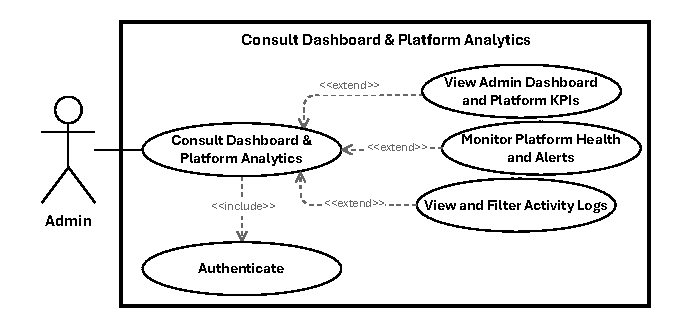
\includegraphics[width=\textwidth]{assets/chapter3/admin-consult-dashboard-and-platform-analytics-use-case}
    \caption{Use Case Approve VM Assignments}
    \label{fig:admin-consult-dashboard-and-platform-analytics-use-case}
\end{figure}
\subsubsubsection{Specification of the Use Case List All VM Assignments}
\begin{table}[H]
    \centering
    \caption{Use Case Specification: List All VM Assignments}
    \begin{tabular}{|p{2.7cm}|p{12.5cm}|}
        \hline
        \textbf{Title}          & List All VM Assignments                                                                 \\
        \hline
        \textbf{Summary}        & Administrator views all VM template assignments to training units with their status     \\
        \hline
        \textbf{Actor}          & Administrator                                                                           \\
        \hline
        \textbf{Precondition}   & The administrator is authenticated with admin privileges                                \\
        \hline
        \textbf{Post-condition} & The administrator views a list of VM assignments with status and configuration details  \\
        \hline
        \textbf{Basic Scenario} & \begin{minipage}[t]{\linewidth}
                                      \begin{enumerate}[topsep=0pt,itemsep=1pt,parsep=0pt,partopsep=0pt]
                                          \item Administrator navigates to the VM Assignments section
                                          \item System retrieves all VM template assignments
                                          \item System displays assignments with template, training path, unit, and status
                                          \item Administrator can filter assignments by status or training path
                                          \item Administrator can view detailed assignment information
                                      \end{enumerate}
                                  \end{minipage} \\
        \hline
        \textbf{Error Scenario} & \begin{minipage}[t]{\linewidth}
                                      \begin{enumerate}[topsep=0pt,itemsep=1pt,parsep=0pt,partopsep=0pt]
                                          \item If no assignments exist, the system displays an empty-state message
                                          \item If the assignment list cannot be retrieved, the system shows an error
                                                notification
                                      \end{enumerate}
                                  \end{minipage}      \\
        \hline
    \end{tabular}
    \label{tab:admin-list-vm-assignments}
\end{table}
\subsubsubsection{Specification of the Use Case View Pending VM Assignments (Duplicate)}
\begin{table}[H]
    \centering
    \caption{Use Case Specification: View Pending VM Assignments}
    \begin{tabular}{|p{2.7cm}|p{12.5cm}|}
        \hline
        \textbf{Title}          & View Pending VM Assignments                                                                    \\
        \hline
        \textbf{Summary}        & Administrator views all pending VM assignment requests awaiting approval                       \\
        \hline
        \textbf{Actor}          & Administrator                                                                                  \\
        \hline
        \textbf{Precondition}   & The administrator is authenticated with admin privileges                                       \\
        \hline
        \textbf{Post-condition} & The administrator views a list of pending VM assignments with teacher and template information \\
        \hline
        \textbf{Basic Scenario} & \begin{minipage}[t]{\linewidth}
                                      \begin{enumerate}[topsep=0pt,itemsep=1pt,parsep=0pt,partopsep=0pt]
                                          \item Administrator navigates to the Pending VM Assignments section
                                          \item System retrieves all pending VM assignment requests
                                          \item System displays assignments with teacher, training path, unit, and requested
                                                template
                                          \item Administrator can filter assignments by teacher or training path
                                          \item Administrator can approve or reject assignments from this view
                                      \end{enumerate}
                                  \end{minipage}      \\
        \hline
        \textbf{Error Scenario} & \begin{minipage}[t]{\linewidth}
                                      \begin{enumerate}[topsep=0pt,itemsep=1pt,parsep=0pt,partopsep=0pt]
                                          \item If no pending assignments exist, the system displays an empty-state message
                                          \item If the assignment list cannot be retrieved, the system shows an error
                                                notification
                                      \end{enumerate}
                                  \end{minipage}       \\
        \hline
    \end{tabular}
    \label{tab:admin-view-pending-vm-assignments-dup}
\end{table}
\subsubsubsection{Specification of the Use Case Approve VM Assignments}
\begin{table}[H]
    \centering
    \caption{Use Case Specification: Approve VM Assignments}
    \begin{tabular}{|p{2.7cm}|p{12.5cm}|}
        \hline
        \textbf{Title}          & Approve VM Assignments                                                                     \\
        \hline
        \textbf{Summary}        & Administrator approves pending VM assignment requests, linking templates to training units \\
        \hline
        \textbf{Actor}          & Administrator                                                                              \\
        \hline
        \textbf{Precondition}   & The administrator is authenticated and has selected pending VM assignment requests         \\
        \hline
        \textbf{Post-condition} & The VM assignments are approved and the teachers are notified of the approvals             \\
        \hline
        \textbf{Basic Scenario} & \begin{minipage}[t]{\linewidth}
                                      \begin{enumerate}[topsep=0pt,itemsep=1pt,parsep=0pt,partopsep=0pt]
                                          \item Administrator selects one or more pending VM assignment requests
                                          \item Administrator reviews the request details and resource requirements
                                          \item Administrator clicks Approve
                                          \item System validates infrastructure capacity for each request
                                          \item System links the VM templates to the training units
                                          \item System updates the request statuses to approved
                                          \item System sends notifications to the teachers
                                      \end{enumerate}
                                  \end{minipage}           \\
        \hline
        \textbf{Error Scenario} & \begin{minipage}[t]{\linewidth}
                                      \begin{enumerate}[topsep=0pt,itemsep=1pt,parsep=0pt,partopsep=0pt]
                                          \item If any requested template no longer exists, the system flags that request as
                                                invalid
                                          \item If infrastructure capacity is insufficient, the system suggests alternative
                                                templates
                                      \end{enumerate}
                                  \end{minipage}  \\
        \hline
    \end{tabular}
    \label{tab:admin-approve-vm-assignments}
\end{table}
\subsubsubsection{Specification of the Use Case Reject VM Assignments}
\begin{table}[H]
    \centering
    \caption{Use Case Specification: Reject VM Assignments}
    \begin{tabular}{|p{2.7cm}|p{12.5cm}|}
        \hline
        \textbf{Title}          & Reject VM Assignments                                                                     \\
        \hline
        \textbf{Summary}        & Administrator rejects pending VM assignment requests and provides feedback to teachers    \\
        \hline
        \textbf{Actor}          & Administrator                                                                             \\
        \hline
        \textbf{Precondition}   & The administrator is authenticated and has selected pending VM assignment requests        \\
        \hline
        \textbf{Post-condition} & The VM assignments are rejected and the teachers are notified with rejection reasons      \\
        \hline
        \textbf{Basic Scenario} & \begin{minipage}[t]{\linewidth}
                                      \begin{enumerate}[topsep=0pt,itemsep=1pt,parsep=0pt,partopsep=0pt]
                                          \item Administrator selects one or more pending VM assignment requests
                                          \item Administrator clicks Reject
                                          \item System displays the rejection form with feedback field
                                          \item Administrator enters rejection feedback explaining the reasons
                                          \item System updates the request statuses to rejected
                                          \item System sends notifications to the teachers with the feedback
                                      \end{enumerate}
                                  \end{minipage}             \\
        \hline
        \textbf{Error Scenario} & \begin{minipage}[t]{\linewidth}
                                      \begin{enumerate}[topsep=0pt,itemsep=1pt,parsep=0pt,partopsep=0pt]
                                          \item If any request is already approved or rejected, the system displays a notice
                                          \item If the rejection fails, the system displays an error and retains the current
                                                state
                                      \end{enumerate}
                                  \end{minipage} \\
        \hline
    \end{tabular}
    \label{tab:admin-reject-vm-assignments}
\end{table}


\subsubsection[Refinement of the Use Case Manage Reservations]{Refinement of the Use Case Manage Reservations} Figure
\ref{fig:admin-manage-reservations-use-case} presents the refinement of the
Use Case Manage Reservations for the Administrator actor. This use case includes
the following sub-use cases:
\begin{figure}[H]
    \centering
    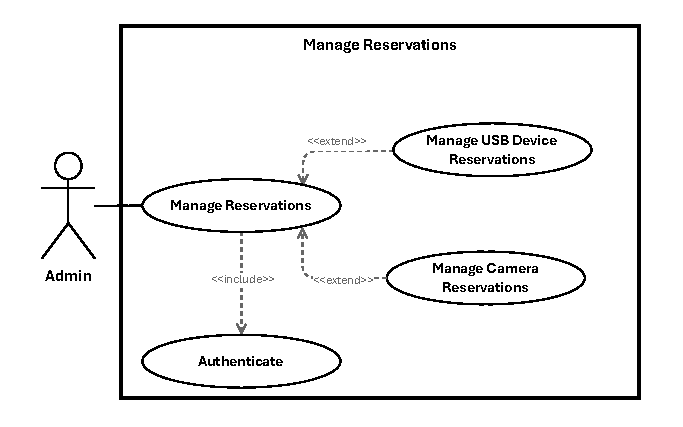
\includegraphics[width=\textwidth]{assets/chapter3/admin-manage-reservations-use-case}
    \caption{Use Case Manage Reservations}
    \label{fig:admin-manage-reservations-use-case}
\end{figure}
\subsubsubsection{Specification of the Use Case Manage USB Device Reservations}
\begin{table}[H]
    \centering
    \caption{Use Case Specification: Manage USB Device Reservations}
    \begin{tabular}{|p{2.7cm}|p{12.5cm}|}
        \hline
        \textbf{Title}          & Manage USB Device Reservations \\
        \hline
        \textbf{Summary}        & Administrator views all USB device reservations across all statuses, filters to pending or upcoming requests, approves or rejects pending reservations with feedback, and blocks device time slots to prevent reservations during maintenance periods \\
        \hline
        \textbf{Actor}          & Administrator \\
        \hline
        \textbf{Precondition}   & The administrator is authenticated with admin privileges \\
        \hline
        \textbf{Post-condition} & USB reservation statuses are updated to approved or rejected and engineers are notified, or a time slot is blocked and the device becomes unavailable for that period \\
        \hline
        \textbf{Basic Scenario} & \begin{minipage}[t]{\linewidth}
            \begin{enumerate}[topsep=0pt,itemsep=1pt,parsep=0pt,partopsep=0pt]
                \item Administrator navigates to the USB Reservations section; system displays all reservations with device, user, status, and time slot; administrator may filter by status or device
                \item Administrator applies the \textbf{Pending} filter to focus on requests awaiting decision; system displays pending reservations with device, user, and requested time slot; administrator may filter by device or user
                \item Administrator applies the \textbf{Upcoming} filter to monitor approved future reservations; system displays approved future reservations with device, user, and scheduled time slot; administrator may filter by date range or device
                \item For \textbf{Approve}: administrator selects a pending request and confirms approval; system validates device availability for the requested time slot, updates the reservation status to approved, and notifies the engineer
                \item For \textbf{Reject}: administrator selects a pending request, enters feedback, and confirms; system updates the status to rejected and sends the feedback to the engineer as a notification
                \item For \textbf{Block Time Slot}: administrator selects a USB device, specifies a date range and reason, and confirms; system creates a blocked time slot for the device and displays the blocked periods
            \end{enumerate}
        \end{minipage} \\
        \hline
        \textbf{Error Scenario} & \begin{minipage}[t]{\linewidth}
            \begin{enumerate}[topsep=0pt,itemsep=1pt,parsep=0pt,partopsep=0pt]
                \item If no reservations exist for the active filter, system displays an appropriate empty state
                \item If any list cannot be retrieved, system shows an error notification
                \item If the device is already reserved for the requested time slot, system suggests an alternative time
                \item If the block time slot conflicts with existing reservations, system displays a conflict warning
                \item If the reservation is already approved or rejected, system displays an explanatory notice
                \item Persistence failures for any action retain the current state and surface a recoverable error
            \end{enumerate}
        \end{minipage} \\
        \hline
    \end{tabular}
    \label{tab:admin-usb-reservations}
\end{table}
\subsubsubsection{Specification of the Use Case Manage VM Reservations}
\begin{table}[H]
    \centering
    \caption{Use Case Specification: Manage VM Reservations}
    \begin{tabular}{|p{2.7cm}|p{12.5cm}|}
        \hline
        \textbf{Title}          & Manage VM Reservations \\
        \hline
        \textbf{Summary}        & Administrator views VM reservation requests across all statuses, filters to pending or upcoming requests, approves or rejects them with feedback, and monitors conflicts with maintenance windows \\
        \hline
        \textbf{Actor}          & Administrator \\
        \hline
        \textbf{Precondition}   & The administrator is authenticated with admin privileges \\
        \hline
        \textbf{Post-condition} & VM reservation statuses are updated to approved or rejected and engineers are notified, or a time slot conflict is surfaced for review \\
        \hline
        \textbf{Basic Scenario} & \begin{minipage}[t]{\linewidth}
            \begin{enumerate}[topsep=0pt,itemsep=1pt,parsep=0pt,partopsep=0pt]
                \item Administrator navigates to the VM Reservations section; system displays all reservations with VM, user, status, and time slot; administrator may filter by status or VM template
                \item Administrator applies the \textbf{Pending} filter to focus on requests awaiting decision; system displays pending VM reservations with engineer, requested template, and requested time slot
                \item Administrator applies the \textbf{Upcoming} filter to monitor approved future VM reservations; system displays approved future reservations with engineer, template, and scheduled time slot
                \item For \textbf{Approve}: administrator selects a pending request and confirms approval; system validates VM availability for the requested time slot, updates the reservation status to approved, and notifies the engineer
                \item For \textbf{Reject}: administrator selects a pending request, enters feedback, and confirms; system updates the status to rejected and sends the feedback to the engineer as a notification
            \end{enumerate}
        \end{minipage} \\
        \hline
        \textbf{Error Scenario} & \begin{minipage}[t]{\linewidth}
            \begin{enumerate}[topsep=0pt,itemsep=1pt,parsep=0pt,partopsep=0pt]
                \item If no reservations exist for the active filter, system displays an appropriate empty state
                \item If any list cannot be retrieved, system shows an error notification
                \item If the VM is already reserved for the requested time slot, system suggests an alternative time
                \item If the reservation conflicts with a maintenance window, system displays a conflict warning
                \item If the reservation is already approved or rejected, system displays an explanatory notice
                \item Persistence failures for any action retain the current state and surface a recoverable error
            \end{enumerate}
        \end{minipage} \\
        \hline
    \end{tabular}
    \label{tab:admin-vm-reservations-detailed}
\end{table}
\subsubsubsection{Specification of the Use Case Manage Camera Reservations}
\begin{table}[H]
    \centering
    \caption{Use Case Specification: Manage Camera Reservations}
    \begin{tabular}{|p{2.7cm}|p{12.5cm}|}
        \hline
        \textbf{Title}          & Manage Camera Reservations \\
        \hline
        \textbf{Summary}        & Administrator views all camera reservations, filters to pending requests, approves or rejects them with feedback, and blocks camera time slots to prevent reservations during maintenance periods \\
        \hline
        \textbf{Actor}          & Administrator \\
        \hline
        \textbf{Precondition}   & The administrator is authenticated with admin privileges \\
        \hline
        \textbf{Post-condition} & Camera reservation statuses are updated to approved or rejected and engineers are notified, or a time slot is blocked and the camera becomes unavailable for that period \\
        \hline
        \textbf{Basic Scenario} & \begin{minipage}[t]{\linewidth}
            \begin{enumerate}[topsep=0pt,itemsep=1pt,parsep=0pt,partopsep=0pt]
                \item Administrator navigates to the Camera Reservations section; system displays all reservations with camera, user, status, and time slot; administrator may filter by status or camera
                \item Administrator applies the \textbf{Pending} filter; system displays pending reservations with camera, user, and requested time slot; administrator may filter by camera or user
                \item For \textbf{Approve}: administrator selects a pending request and confirms approval; system validates camera availability for the requested time slot, updates the reservation status to approved, and notifies the engineer
                \item For \textbf{Reject}: administrator selects a pending request, enters feedback, and confirms; system updates the status to rejected and sends the feedback to the engineer as a notification
                \item For \textbf{Block Time Slot}: administrator selects a camera, specifies a date range and reason, and confirms; system creates a blocked time slot for the camera and displays the blocked periods
            \end{enumerate}
        \end{minipage} \\
        \hline
        \textbf{Error Scenario} & \begin{minipage}[t]{\linewidth}
            \begin{enumerate}[topsep=0pt,itemsep=1pt,parsep=0pt,partopsep=0pt]
                \item If no reservations exist for the active filter, system displays an appropriate empty state
                \item If any list cannot be retrieved, system shows an error notification
                \item If the camera is already reserved for the requested time slot, system suggests an alternative time
                \item If the block time slot conflicts with existing reservations, system displays a conflict warning
                \item If the reservation is already approved or rejected, system displays an explanatory notice
                \item Persistence failures for any action retain the current state and surface a recoverable error
            \end{enumerate}
        \end{minipage} \\
        \hline
    \end{tabular}
    \label{tab:admin-camera-reservations}
\end{table}


\subsubsubsection{Specification of the Use Case List All USB Reservations}
\begin{table}[H]
    \centering
    \caption{Use Case Specification: List All USB Reservations}
    \begin{tabular}{|p{2.7cm}|p{12.5cm}|}
        \hline
        \textbf{Title}          & List All USB Reservations                                                                 \\
        \hline
        \textbf{Summary}        & Administrator views all USB device reservations with their status, user, and time slot    \\
        \hline
        \textbf{Actor}          & Administrator                                                                             \\
        \hline
        \textbf{Precondition}   & The administrator is authenticated with admin privileges                                  \\
        \hline
        \textbf{Post-condition} & The administrator views a list of USB reservations with status and scheduling information \\
        \hline
        \textbf{Basic Scenario} & \begin{minipage}[t]{\linewidth}
                                      \begin{enumerate}[topsep=0pt,itemsep=1pt,parsep=0pt,partopsep=0pt]
                                          \item Administrator navigates to the USB Reservations section
                                          \item System retrieves all USB device reservations
                                          \item System displays reservations with device, user, status, and time slot
                                          \item Administrator can filter reservations by status or device
                                          \item Administrator can view detailed reservation information
                                      \end{enumerate}
                                  \end{minipage}        \\
        \hline
        \textbf{Error Scenario} & \begin{minipage}[t]{\linewidth}
                                      \begin{enumerate}[topsep=0pt,itemsep=1pt,parsep=0pt,partopsep=0pt]
                                          \item If no reservations exist, the system displays an empty-state message
                                          \item If the reservation list cannot be retrieved, the system shows an error
                                                notification
                                      \end{enumerate}
                                  \end{minipage}       \\
        \hline
    \end{tabular}
    \label{tab:admin-list-usb-reservations}
\end{table}
\subsubsubsection{Specification of the Use Case View Pending Reservations}
\begin{table}[H]
    \centering
    \caption{Use Case Specification: View Pending Reservations}
    \begin{tabular}{|p{2.7cm}|p{12.5cm}|}
        \hline
        \textbf{Title}          & View Pending Reservations                                                                 \\
        \hline
        \textbf{Summary}        & Administrator views all pending USB device reservation requests awaiting approval         \\
        \hline
        \textbf{Actor}          & Administrator                                                                             \\
        \hline
        \textbf{Precondition}   & The administrator is authenticated with admin privileges                                  \\
        \hline
        \textbf{Post-condition} & The administrator views a list of pending reservations with user and device information   \\
        \hline
        \textbf{Basic Scenario} & \begin{minipage}[t]{\linewidth}
                                      \begin{enumerate}[topsep=0pt,itemsep=1pt,parsep=0pt,partopsep=0pt]
                                          \item Administrator navigates to the Pending Reservations section
                                          \item System retrieves all pending USB reservation requests
                                          \item System displays reservations with device, user, and requested time slot
                                          \item Administrator can filter reservations by device or user
                                          \item Administrator can approve or reject reservations from this view
                                      \end{enumerate}
                                  \end{minipage}      \\
        \hline
        \textbf{Error Scenario} & \begin{minipage}[t]{\linewidth}
                                      \begin{enumerate}[topsep=0pt,itemsep=1pt,parsep=0pt,partopsep=0pt]
                                          \item If no pending reservations exist, the system displays an empty-state message
                                          \item If the reservation list cannot be retrieved, the system shows an error
                                                notification
                                      \end{enumerate}
                                  \end{minipage} \\
        \hline
    \end{tabular}
    \label{tab:admin-view-pending-reservations}
\end{table}
\subsubsubsection{Specification of the Use Case View Upcoming Reservations}
\begin{table}[H]
    \centering
    \caption{Use Case Specification: View Upcoming Reservations}
    \begin{tabular}{|p{2.7cm}|p{12.5cm}|}
        \hline
        \textbf{Title}          & View Upcoming Reservations                                                                 \\
        \hline
        \textbf{Summary}        & Administrator views all approved USB device reservations scheduled for the future          \\
        \hline
        \textbf{Actor}          & Administrator                                                                              \\
        \hline
        \textbf{Precondition}   & The administrator is authenticated with admin privileges                                   \\
        \hline
        \textbf{Post-condition} & The administrator views a list of upcoming reservations with scheduling details            \\
        \hline
        \textbf{Basic Scenario} & \begin{minipage}[t]{\linewidth}
                                      \begin{enumerate}[topsep=0pt,itemsep=1pt,parsep=0pt,partopsep=0pt]
                                          \item Administrator navigates to the Upcoming Reservations section
                                          \item System retrieves all approved future USB reservations
                                          \item System displays reservations with device, user, and scheduled time slot
                                          \item Administrator can filter reservations by date range or device
                                          \item Administrator can view detailed reservation information
                                      \end{enumerate}
                                  \end{minipage}       \\
        \hline
        \textbf{Error Scenario} & \begin{minipage}[t]{\linewidth}
                                      \begin{enumerate}[topsep=0pt,itemsep=1pt,parsep=0pt,partopsep=0pt]
                                          \item If no upcoming reservations exist, the system displays an empty-state message
                                          \item If the reservation list cannot be retrieved, the system shows an error
                                                notification
                                      \end{enumerate}
                                  \end{minipage} \\
        \hline
    \end{tabular}
    \label{tab:admin-view-upcoming-reservations}
\end{table}
\subsubsubsection{Specification of the Use Case Approve USB Reservation}
\begin{table}[H]
    \centering
    \caption{Use Case Specification: Approve USB Reservation}
    \begin{tabular}{|p{2.7cm}|p{12.5cm}|}
        \hline
        \textbf{Title}          & Approve USB Reservation                                                                  \\
        \hline
        \textbf{Summary}        & Administrator approves a pending USB device reservation request                          \\
        \hline
        \textbf{Actor}          & Administrator                                                                            \\
        \hline
        \textbf{Precondition}   & The administrator is authenticated and has selected a pending USB reservation request    \\
        \hline
        \textbf{Post-condition} & The USB reservation is approved and the engineer is notified of the approval             \\
        \hline
        \textbf{Basic Scenario} & \begin{minipage}[t]{\linewidth}
                                      \begin{enumerate}[topsep=0pt,itemsep=1pt,parsep=0pt,partopsep=0pt]
                                          \item Administrator selects a pending USB reservation request
                                          \item Administrator reviews the request details and device availability
                                          \item Administrator clicks Approve
                                          \item System validates device availability for the requested time slot
                                          \item System updates the reservation status to approved
                                          \item System sends a notification to the engineer
                                      \end{enumerate}
                                  \end{minipage}           \\
        \hline
        \textbf{Error Scenario} & \begin{minipage}[t]{\linewidth}
                                      \begin{enumerate}[topsep=0pt,itemsep=1pt,parsep=0pt,partopsep=0pt]
                                          \item If the device is already reserved for the time slot, the system suggests an
                                                alternative time
                                          \item If the approval fails, the system displays an error and retains the pending
                                                state
                                      \end{enumerate}
                                  \end{minipage} \\
        \hline
    \end{tabular}
    \label{tab:admin-approve-usb-reservation}
\end{table}
\subsubsubsection{Specification of the Use Case Reject USB Reservation}
\begin{table}[H]
    \centering
    \caption{Use Case Specification: Reject USB Reservation}
    \begin{tabular}{|p{2.7cm}|p{12.5cm}|}
        \hline
        \textbf{Title}          & Reject USB Reservation                                                                    \\
        \hline
        \textbf{Summary}        & Administrator rejects a pending USB device reservation request and provides feedback      \\
        \hline
        \textbf{Actor}          & Administrator                                                                             \\
        \hline
        \textbf{Precondition}   & The administrator is authenticated and has selected a pending USB reservation request     \\
        \hline
        \textbf{Post-condition} & The USB reservation is rejected and the engineer is notified with the rejection reason    \\
        \hline
        \textbf{Basic Scenario} & \begin{minipage}[t]{\linewidth}
                                      \begin{enumerate}[topsep=0pt,itemsep=1pt,parsep=0pt,partopsep=0pt]
                                          \item Administrator selects a pending USB reservation request
                                          \item Administrator clicks Reject
                                          \item System displays the rejection form with feedback field
                                          \item Administrator enters rejection feedback explaining the reasons
                                          \item System updates the reservation status to rejected
                                          \item System sends a notification to the engineer with the feedback
                                      \end{enumerate}
                                  \end{minipage}               \\
        \hline
        \textbf{Error Scenario} & \begin{minipage}[t]{\linewidth}
                                      \begin{enumerate}[topsep=0pt,itemsep=1pt,parsep=0pt,partopsep=0pt]
                                          \item If the reservation is already approved or rejected, the system displays a
                                                notice
                                          \item If the rejection fails, the system displays an error and retains the current
                                                state
                                      \end{enumerate}
                                  \end{minipage} \\
        \hline
    \end{tabular}
    \label{tab:admin-reject-usb-reservation}
\end{table}
\subsubsubsection{Specification of the Use Case Block USB Device Time Slot}
\begin{table}[H]
    \centering
    \caption{Use Case Specification: Block USB Device Time Slot}
    \begin{tabular}{|p{2.7cm}|p{12.5cm}|}
        \hline
        \textbf{Title}          & Block USB Device Time Slot                                                                            \\
        \hline
        \textbf{Summary}        & Administrator blocks a specific time slot for a USB device to prevent reservations during maintenance \\
        \hline
        \textbf{Actor}          & Administrator                                                                                         \\
        \hline
        \textbf{Precondition}   & The administrator is authenticated and has selected a USB device                                      \\
        \hline
        \textbf{Post-condition} & The USB device time slot is blocked and no reservations can be made for that period                   \\
        \hline
        \textbf{Basic Scenario} & \begin{minipage}[t]{\linewidth}
                                      \begin{enumerate}[topsep=0pt,itemsep=1pt,parsep=0pt,partopsep=0pt]
                                          \item Administrator selects a USB device from the device list
                                          \item Administrator clicks Block Time Slot
                                          \item System displays the time slot blocking form
                                          \item Administrator selects the date range and time to block
                                          \item Administrator enters a reason for the block
                                          \item System creates a blocked time slot for the device
                                          \item System confirms the block and displays the blocked periods
                                      \end{enumerate}
                                  \end{minipage}                               \\
        \hline
        \textbf{Error Scenario} & \begin{minipage}[t]{\linewidth}
                                      \begin{enumerate}[topsep=0pt,itemsep=1pt,parsep=0pt,partopsep=0pt]
                                          \item If the time slot conflicts with existing reservations, the system displays a
                                                conflict warning
                                          \item If the block creation fails, the system displays an error and retains the
                                                current state
                                      \end{enumerate}
                                  \end{minipage}             \\
        \hline
    \end{tabular}
    \label{tab:admin-block-usb-time-slot}
\end{table}
\subsubsubsection{Specification of the Use Case List Camera Reservations}
\begin{table}[H]
    \centering
    \caption{Use Case Specification: List Camera Reservations}
    \begin{tabular}{|p{2.7cm}|p{12.5cm}|}
        \hline
        \textbf{Title}          & List Camera Reservations                                                                     \\
        \hline
        \textbf{Summary}        & Administrator views all camera reservations with their status, user, and time slot           \\
        \hline
        \textbf{Actor}          & Administrator                                                                                \\
        \hline
        \textbf{Precondition}   & The administrator is authenticated with admin privileges                                     \\
        \hline
        \textbf{Post-condition} & The administrator views a list of camera reservations with status and scheduling information \\
        \hline
        \textbf{Basic Scenario} & \begin{minipage}[t]{\linewidth}
                                      \begin{enumerate}[topsep=0pt,itemsep=1pt,parsep=0pt,partopsep=0pt]
                                          \item Administrator navigates to the Camera Reservations section
                                          \item System retrieves all camera reservations
                                          \item System displays reservations with camera, user, status, and time slot
                                          \item Administrator can filter reservations by status or camera
                                          \item Administrator can view detailed reservation information
                                      \end{enumerate}
                                  \end{minipage}           \\
        \hline
        \textbf{Error Scenario} & \begin{minipage}[t]{\linewidth}
                                      \begin{enumerate}[topsep=0pt,itemsep=1pt,parsep=0pt,partopsep=0pt]
                                          \item If no reservations exist, the system displays an empty-state message
                                          \item If the reservation list cannot be retrieved, the system shows an error
                                                notification
                                      \end{enumerate}
                                  \end{minipage}          \\
        \hline
    \end{tabular}
    \label{tab:admin-list-camera-reservations}
\end{table}
\subsubsubsection{Specification of the Use Case View Pending Camera Reservations}
\begin{table}[H]
    \centering
    \caption{Use Case Specification: View Pending Camera Reservations}
    \begin{tabular}{|p{2.7cm}|p{12.5cm}|}
        \hline
        \textbf{Title}          & View Pending Camera Reservations                                                               \\
        \hline
        \textbf{Summary}        & Administrator views all pending camera reservation requests awaiting approval                  \\
        \hline
        \textbf{Actor}          & Administrator                                                                                  \\
        \hline
        \textbf{Precondition}   & The administrator is authenticated with admin privileges                                       \\
        \hline
        \textbf{Post-condition} & The administrator views a list of pending camera reservations with user and camera information \\
        \hline
        \textbf{Basic Scenario} & \begin{minipage}[t]{\linewidth}
                                      \begin{enumerate}[topsep=0pt,itemsep=1pt,parsep=0pt,partopsep=0pt]
                                          \item Administrator navigates to the Pending Camera Reservations section
                                          \item System retrieves all pending camera reservation requests
                                          \item System displays reservations with camera, user, and requested time slot
                                          \item Administrator can filter reservations by camera or user
                                          \item Administrator can approve or reject reservations from this view
                                      \end{enumerate}
                                  \end{minipage}           \\
        \hline
        \textbf{Error Scenario} & \begin{minipage}[t]{\linewidth}
                                      \begin{enumerate}[topsep=0pt,itemsep=1pt,parsep=0pt,partopsep=0pt]
                                          \item If no pending reservations exist, the system displays an empty-state message
                                          \item If the reservation list cannot be retrieved, the system shows an error
                                                notification
                                      \end{enumerate}
                                  \end{minipage}      \\
        \hline
    \end{tabular}
    \label{tab:admin-view-pending-camera-reservations}
\end{table}
\subsubsubsection{Specification of the Use Case Approve Camera Reservation}
\begin{table}[H]
    \centering
    \caption{Use Case Specification: Approve Camera Reservation}
    \begin{tabular}{|p{2.7cm}|p{12.5cm}|}
        \hline
        \textbf{Title}          & Approve Camera Reservation                                                               \\
        \hline
        \textbf{Summary}        & Administrator approves a pending camera reservation request                              \\
        \hline
        \textbf{Actor}          & Administrator                                                                            \\
        \hline
        \textbf{Precondition}   & The administrator is authenticated and has selected a pending camera reservation request \\
        \hline
        \textbf{Post-condition} & The camera reservation is approved and the engineer is notified of the approval          \\
        \hline
        \textbf{Basic Scenario} & \begin{minipage}[t]{\linewidth}
                                      \begin{enumerate}[topsep=0pt,itemsep=1pt,parsep=0pt,partopsep=0pt]
                                          \item Administrator selects a pending camera reservation request
                                          \item Administrator reviews the request details and camera availability
                                          \item Administrator clicks Approve
                                          \item System validates camera availability for the requested time slot
                                          \item System updates the reservation status to approved
                                          \item System sends a notification to the engineer
                                      \end{enumerate}
                                  \end{minipage}           \\
        \hline
        \textbf{Error Scenario} & \begin{minipage}[t]{\linewidth}
                                      \begin{enumerate}[topsep=0pt,itemsep=1pt,parsep=0pt,partopsep=0pt]
                                          \item If the camera is already reserved for the time slot, the system suggests an
                                                alternative time
                                          \item If the approval fails, the system displays an error and retains the pending
                                                state
                                      \end{enumerate}
                                  \end{minipage} \\
        \hline
    \end{tabular}
    \label{tab:admin-approve-camera-reservation}
\end{table}
\subsubsubsection{Specification of the Use Case Dedicate / Remove Device Dedication}
\begin{table}[H]
    \centering
    \caption{Use Case Specification: Dedicate / Remove Device Dedication}
    \begin{tabular}{|p{2.7cm}|p{12.5cm}|}
        \hline
        	extbf{Title}          & Dedicate / Remove Device Dedication \\ \hline
        	extbf{Summary}        & Administrator assigns a USB device permanently to a VM so the device auto-attaches when that VM starts, or removes that assignment. System performs necessary cleanup (detach/unbind) before persisting dedication metadata and synchronises linked camera records where applicable. \\ \hline
        	extbf{Actor}          & Administrator \\ \hline
        	extbf{Precondition}   & Administrator authenticated and authorised; the target USB device exists; for dedication the request includes valid \texttt{vmid}, \texttt{node}, and \texttt{server\_id} referencing an existing Proxmox server. \\ \hline
        	extbf{Post-condition} & \begin{minipage}[t]{\linewidth}
                                      \begin{enumerate}[topsep=0pt,itemsep=0pt,parsep=0pt,partopsep=0pt]
                                          \item (Dedicate) Device fields \texttt{dedicated\_vmid}, \texttt{dedicated\_node}, \texttt{dedicated\_server\_id} persisted; device is left available for auto-attach on VM start.
                                          \item Any existing attachment or gateway binding is cleared prior to persistence.
                                          \item Linked camera (if present) is assigned to the VM and streaming may be stopped.
                                          \item (Remove) Dedicated fields cleared and any camera assignment removed.
                                      \end{enumerate}
                                  \end{minipage} \\ \hline
        	extbf{Basic Scenario} & \begin{minipage}[t]{\linewidth}
                                      \begin{enumerate}[topsep=0pt,itemsep=1pt,parsep=0pt,partopsep=0pt]
                                          \item Administrator opens the device in admin hardware UI and chooses \textit{Dedicate Device}.
                                          \item Administrator submits \texttt{vmid}, \texttt{node}, and \texttt{server\_id}.
                                          \item Controller authorises the request and validates inputs.
                                          \item Controller loads the Proxmox server record and calls GatewayService::dedicateDeviceToVm(...).
                                          \item Service detaches the device if attached and unbinds it if bound on the gateway.
                                          \item Service persists dedication metadata via UsbDeviceRepository::setDedicatedVm(...).
                                          \item If the device is a camera, the service assigns the camera to the VM and attempts to stop any active stream, updating camera state.
                                          \item Controller returns HTTP 200 with the updated UsbDeviceResource and confirmation message.
                                      \end{enumerate}
                                  \end{minipage} \\ \hline
        	extbf{Error Scenario} & \begin{minipage}[t]{\linewidth}
                                      \begin{enumerate}[topsep=0pt,itemsep=1pt,parsep=0pt,partopsep=0pt]
                                          \item If the initiator is not authorised, Controller returns HTTP 403; no changes made.
                                          \item If input validation fails (missing or invalid \texttt{vmid}, \texttt{node}, or \texttt{server\_id}), Controller returns HTTP 422 and no change is persisted.
                                          \item If the device is not dedicated when a remove request is issued, Controller returns HTTP 422 with message "Device is not dedicated to any VM".
                                          \item If detach/unbind or persistence fails, Service aborts, logs the error, and Controller returns an error response; partial cleanup may require manual reconciliation.
                                          \item If the device is currently in use (attached to an active session), the system may prevent dedication changes until released.
                                      \end{enumerate}
                                  \end{minipage} \\ \hline
    \end{tabular}
    \label{tab:admin-dedicate-remove-device}
\end{table}
                                  \end{minipage}                           \\
        \hline
        \textbf{Error Scenario} & \begin{minipage}[t]{\linewidth}
                                      \begin{enumerate}[topsep=0pt,itemsep=1pt,parsep=0pt,partopsep=0pt]
                                          \item If the time slot conflicts with existing reservations, the system displays a
                                                conflict warning
                                          \item If the block creation fails, the system displays an error and retains the
                                                current state
                                      \end{enumerate}
                                  \end{minipage}         \\
        \hline
    \end{tabular}
    \label{tab:admin-block-camera-time-slot}
\end{table}


\subsubsection[Refinement of the Use Case Manage Payout \& Refunds]{Refinement of the Use Case Manage Payout \& Refunds} Figure
\ref{fig:admin-manage-payout-and-refunds-use-case} presents the refinement of the
Use Case Manage Payout \& Refunds for the Administrator actor. This use case includes
the following sub-use cases:
\begin{figure}[H]
    \centering
    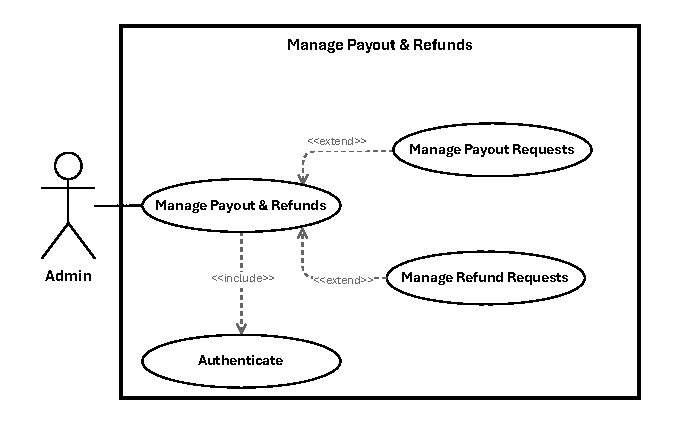
\includegraphics[width=\textwidth]{assets/chapter3/admin-manage-payout-and-refunds-use-case}
    \caption{Use Case Manage Payout \& Refunds}
    \label{fig:admin-manage-payout-and-refunds-use-case}
\end{figure}
\subsubsubsection{Specification of the Use Case Manage Payout Requests}
\begin{table}[H]
    \centering
    \caption{Use Case Specification: Manage Payout Requests}
    \begin{tabular}{|p{2.7cm}|p{12.5cm}|}
        \hline
        \textbf{Title}          & Manage Payout Requests \\
        \hline
        \textbf{Summary}        & Administrator views all teacher payout requests, approves or rejects pending ones with feedback, processes approved transfers through the payment processor, and exports payout data for accounting purposes \\
        \hline
        \textbf{Actor}          & Administrator \\
        \hline
        \textbf{Precondition}   & The administrator is authenticated with admin privileges \\
        \hline
        \textbf{Post-condition} & Payout statuses are updated to approved, rejected, or processing; fund transfers are initiated for approved payouts; teachers are notified of all decisions; and payout reports are available for download \\
        \hline
        \textbf{Basic Scenario} & \begin{minipage}[t]{\linewidth}
            \begin{enumerate}[topsep=0pt,itemsep=1pt,parsep=0pt,partopsep=0pt]
                \item Administrator navigates to the Payout Requests section; system displays all requests with teacher, amount, status, and request date; administrator may filter by status or teacher
                \item For \textbf{Approve}: administrator selects a pending request, reviews payout details and teacher earnings history, and confirms approval; system validates the payout amount and teacher account, updates the status to approved, and notifies the teacher
                \item For \textbf{Reject}: administrator selects a pending request, enters feedback, and confirms; system updates the status to rejected and sends the feedback to the teacher as a notification
                \item For \textbf{Process / Transfer}: administrator selects an approved request and confirms the transfer; system initiates the transfer through the payment processor, updates the status to processing, and logs the action for audit purposes
                \item For \textbf{Export Report}: administrator applies filters (date range, status, teacher) and clicks Export; system generates and offers the report for download in CSV, PDF, or Excel format
            \end{enumerate}
        \end{minipage} \\
        \hline
        \textbf{Error Scenario} & \begin{minipage}[t]{\linewidth}
            \begin{enumerate}[topsep=0pt,itemsep=1pt,parsep=0pt,partopsep=0pt]
                \item If no payout requests exist or the list cannot be retrieved, system displays an appropriate empty state or error notification
                \item If a request is already approved or rejected, system displays an explanatory notice
                \item Processing is blocked if the payout is not in approved status
                \item If the transfer fails, system displays an error and marks the payout for manual review
                \item If no data matches the export filters, system displays an empty state; if report generation fails, system shows an error notification
                \item Persistence failures for any action retain the current state and surface a recoverable error
            \end{enumerate}
        \end{minipage} \\
        \hline
    \end{tabular}
    \label{tab:admin-payout-requests}
\end{table}
\subsubsubsection{Specification of the Use Case Manage Refund Requests}
\begin{table}[H]
    \centering
    \caption{Use Case Specification: Manage Refund Requests}
    \begin{tabular}{|p{2.7cm}|p{12.5cm}|}
        \hline
        \textbf{Title}          & Manage Refund Requests \\
        \hline
        \textbf{Summary}        & Administrator views pending refund requests and the full refund history, approves or rejects pending ones, and executes Stripe refunds manually when automatic processing has failed \\
        \hline
        \textbf{Actor}          & Administrator \\
        \hline
        \textbf{Precondition}   & The administrator is authenticated with admin privileges \\
        \hline
        \textbf{Post-condition} & Refund statuses are updated to approved, rejected, or completed; Stripe refunds are initiated or executed manually; engineers are notified of all decisions \\
        \hline
        \textbf{Basic Scenario} & \begin{minipage}[t]{\linewidth}
            \begin{enumerate}[topsep=0pt,itemsep=1pt,parsep=0pt,partopsep=0pt]
                \item Administrator navigates to the Refund Requests section; system displays all pending requests with engineer, amount, status, and request date; administrator may filter by status or engineer
                \item Administrator navigates to the Refunds History section to review the complete transaction history; system displays all processed refunds with engineer, amount, status, and processing date; administrator may filter by status, date range, or engineer
                \item For \textbf{Approve}: administrator selects a pending request, reviews the refund details and payment information, and confirms approval; system validates eligibility and amount, updates the status to approved, initiates the Stripe refund through the API, and notifies the engineer
                \item For \textbf{Reject}: administrator selects a pending request, enters feedback, and confirms; system updates the status to rejected and sends the feedback to the engineer as a notification
                \item For \textbf{Execute Stripe Refund} (manual fallback): administrator selects an approved request marked for manual processing and confirms execution; system calls the Stripe API, updates the refund status based on the result, and logs the action for audit purposes
            \end{enumerate}
        \end{minipage} \\
        \hline
        \textbf{Error Scenario} & \begin{minipage}[t]{\linewidth}
            \begin{enumerate}[topsep=0pt,itemsep=1pt,parsep=0pt,partopsep=0pt]
                \item If no refund requests or history entries exist, or lists cannot be retrieved, system displays an appropriate empty state or error notification
                \item If a request is already approved or rejected, system displays an explanatory notice
                \item If the Stripe refund API call fails during approval, system logs the error and marks the refund for manual processing
                \item If the Stripe API call fails during manual execution, system displays an error and marks the refund for retry
                \item If the original payment cannot be refunded, system displays an error with details
                \item Persistence failures for any action retain the current state and surface a recoverable error
            \end{enumerate}
        \end{minipage} \\
        \hline
    \end{tabular}
    \label{tab:admin-refund-requests}
\end{table}


\subsubsubsection{Specification of the Use Case List Payout Requests}
\begin{table}[H]
    \centering
    \caption{Use Case Specification: List Payout Requests}
    \begin{tabular}{|p{2.7cm}|p{12.5cm}|}
        \hline
        \textbf{Title}          & List Payout Requests                                                                           \\
        \hline
        \textbf{Summary}        & Administrator views all payout requests submitted by teachers with their status and amounts    \\
        \hline
        \textbf{Actor}          & Administrator                                                                                  \\
        \hline
        \textbf{Precondition}   & The administrator is authenticated with admin privileges                                       \\
        \hline
        \textbf{Post-condition} & The administrator views a list of payout requests with status, teacher, and amount information \\
        \hline
        \textbf{Basic Scenario} & \begin{minipage}[t]{\linewidth}
                                      \begin{enumerate}[topsep=0pt,itemsep=1pt,parsep=0pt,partopsep=0pt]
                                          \item Administrator navigates to the Payout Requests section
                                          \item System retrieves all payout requests
                                          \item System displays requests with teacher, amount, status, and request date
                                          \item Administrator can filter requests by status or teacher
                                          \item Administrator can view detailed payout request information
                                      \end{enumerate}
                                  \end{minipage}           \\
        \hline
        \textbf{Error Scenario} & \begin{minipage}[t]{\linewidth}
                                      \begin{enumerate}[topsep=0pt,itemsep=1pt,parsep=0pt,partopsep=0pt]
                                          \item If no payout requests exist, the system displays an empty-state message
                                          \item If the payout list cannot be retrieved, the system shows an error notification
                                      \end{enumerate}
                                  \end{minipage}    \\
        \hline
    \end{tabular}
    \label{tab:admin-list-payout-requests}
\end{table}
\subsubsubsection{Specification of the Use Case Export Payouts Report}
\begin{table}[H]
    \centering
    \caption{Use Case Specification: Export Payouts Report}
    \begin{tabular}{|p{2.7cm}|p{12.5cm}|}
        \hline
        \textbf{Title}          & Export Payouts Report                                                                   \\
        \hline
        \textbf{Summary}        & Administrator exports a report of payout requests for accounting or analysis purposes   \\
        \hline
        \textbf{Actor}          & Administrator                                                                           \\
        \hline
        \textbf{Precondition}   & The administrator is authenticated and has selected payout requests to export           \\
        \hline
        \textbf{Post-condition} & A payout report file is generated and downloaded in the requested format                \\
        \hline
        \textbf{Basic Scenario} & \begin{minipage}[t]{\linewidth}
                                      \begin{enumerate}[topsep=0pt,itemsep=1pt,parsep=0pt,partopsep=0pt]
                                          \item Administrator navigates to the Payout Requests section
                                          \item Administrator applies filters for the report (date range, status, teacher)
                                          \item Administrator clicks Export Report
                                          \item System generates the report with selected payout data
                                          \item System offers download options: CSV, PDF, or Excel
                                          \item Administrator selects the format and downloads the report
                                      \end{enumerate}
                                  \end{minipage} \\
        \hline
        \textbf{Error Scenario} & \begin{minipage}[t]{\linewidth}
                                      \begin{enumerate}[topsep=0pt,itemsep=1pt,parsep=0pt,partopsep=0pt]
                                          \item If no data matches the filters, the system displays an empty-state message
                                          \item If the report generation fails, the system shows an error notification
                                      \end{enumerate}
                                  \end{minipage} \\
        \hline
    \end{tabular}
    \label{tab:admin-export-payouts-report}
\end{table}
\subsubsubsection{Specification of the Use Case Approve Payout Request}
\begin{table}[H]
    \centering
    \caption{Use Case Specification: Approve Payout Request}
    \begin{tabular}{|p{2.7cm}|p{12.5cm}|}
        \hline
        \textbf{Title}          & Approve Payout Request                                                                    \\
        \hline
        \textbf{Summary}        & Administrator approves a pending payout request for a teacher                             \\
        \hline
        \textbf{Actor}          & Administrator                                                                             \\
        \hline
        \textbf{Precondition}   & The administrator is authenticated and has selected a pending payout request              \\
        \hline
        \textbf{Post-condition} & The payout request is approved and the teacher is notified of the approval                \\
        \hline
        \textbf{Basic Scenario} & \begin{minipage}[t]{\linewidth}
                                      \begin{enumerate}[topsep=0pt,itemsep=1pt,parsep=0pt,partopsep=0pt]
                                          \item Administrator selects a pending payout request
                                          \item Administrator reviews the payout details and teacher earnings history
                                          \item Administrator clicks Approve
                                          \item System validates the payout amount and teacher account
                                          \item System updates the payout status to approved
                                          \item System sends a notification to the teacher
                                      \end{enumerate}
                                  \end{minipage}        \\
        \hline
        \textbf{Error Scenario} & \begin{minipage}[t]{\linewidth}
                                      \begin{enumerate}[topsep=0pt,itemsep=1pt,parsep=0pt,partopsep=0pt]
                                          \item If the payout request is already approved or rejected, the system displays a
                                                notice
                                          \item If the approval fails, the system displays an error and retains the current
                                                state
                                      \end{enumerate}
                                  \end{minipage} \\
        \hline
    \end{tabular}
    \label{tab:admin-approve-payout-request}
\end{table}
\subsubsubsection{Specification of the Use Case Reject Payout Request}
\begin{table}[H]
    \centering
    \caption{Use Case Specification: Reject Payout Request}
    \begin{tabular}{|p{2.7cm}|p{12.5cm}|}
        \hline
        \textbf{Title}          & Reject Payout Request                                                                     \\
        \hline
        \textbf{Summary}        & Administrator rejects a pending payout request and provides feedback to the teacher       \\
        \hline
        \textbf{Actor}          & Administrator                                                                             \\
        \hline
        \textbf{Precondition}   & The administrator is authenticated and has selected a pending payout request              \\
        \hline
        \textbf{Post-condition} & The payout request is rejected and the teacher is notified with the rejection reason      \\
        \hline
        \textbf{Basic Scenario} & \begin{minipage}[t]{\linewidth}
                                      \begin{enumerate}[topsep=0pt,itemsep=1pt,parsep=0pt,partopsep=0pt]
                                          \item Administrator selects a pending payout request
                                          \item Administrator clicks Reject
                                          \item System displays the rejection form with feedback field
                                          \item Administrator enters rejection feedback explaining the reasons
                                          \item System updates the payout status to rejected
                                          \item System sends a notification to the teacher with the feedback
                                      \end{enumerate}
                                  \end{minipage}               \\
        \hline
        \textbf{Error Scenario} & \begin{minipage}[t]{\linewidth}
                                      \begin{enumerate}[topsep=0pt,itemsep=1pt,parsep=0pt,partopsep=0pt]
                                          \item If the payout request is already approved or rejected, the system displays a
                                                notice
                                          \item If the rejection fails, the system displays an error and retains the current
                                                state
                                      \end{enumerate}
                                  \end{minipage} \\
        \hline
    \end{tabular}
    \label{tab:admin-reject-payout-request}
\end{table}
\subsubsubsection{Specification of the Use Case Process / Transfer Payout}
\begin{table}[H]
    \centering
    \caption{Use Case Specification: Process / Transfer Payout}
    \begin{tabular}{|p{2.7cm}|p{12.5cm}|}
        \hline
        \textbf{Title}          & Process / Transfer Payout                                                                    \\
        \hline
        \textbf{Summary}        & Administrator initiates the actual transfer of funds for an approved payout request          \\
        \hline
        \textbf{Actor}          & Administrator                                                                                \\
        \hline
        \textbf{Precondition}   & The administrator is authenticated and has selected an approved payout request               \\
        \hline
        \textbf{Post-condition} & The payout transfer is initiated and the payout status is updated to processing or completed \\
        \hline
        \textbf{Basic Scenario} & \begin{minipage}[t]{\linewidth}
                                      \begin{enumerate}[topsep=0pt,itemsep=1pt,parsep=0pt,partopsep=0pt]
                                          \item Administrator selects an approved payout request
                                          \item Administrator clicks Process Payout
                                          \item System displays the payout details and transfer options
                                          \item Administrator confirms the transfer
                                          \item System initiates the transfer through the payment processor
                                          \item System updates the payout status to processing
                                          \item System logs the transfer for audit purposes
                                      \end{enumerate}
                                  \end{minipage}                     \\
        \hline
        \textbf{Error Scenario} & \begin{minipage}[t]{\linewidth}
                                      \begin{enumerate}[topsep=0pt,itemsep=1pt,parsep=0pt,partopsep=0pt]
                                          \item If the payout is not approved, the system prevents processing
                                          \item If the transfer fails, the system displays an error and marks the payout for
                                                manual review
                                      \end{enumerate}
                                  \end{minipage}    \\
        \hline
    \end{tabular}
    \label{tab:admin-process-payout}
\end{table}
\subsubsubsection{Specification of the Use Case List Refund Requests}
\begin{table}[H]
    \centering
    \caption{Use Case Specification: List Refund Requests}
    \begin{tabular}{|p{2.7cm}|p{12.5cm}|}
        \hline
        \textbf{Title}          & List Refund Requests                                                                            \\
        \hline
        \textbf{Summary}        & Administrator views all refund requests submitted by engineers with their status and amounts    \\
        \hline
        \textbf{Actor}          & Administrator                                                                                   \\
        \hline
        \textbf{Precondition}   & The administrator is authenticated with admin privileges                                        \\
        \hline
        \textbf{Post-condition} & The administrator views a list of refund requests with status, engineer, and amount information \\
        \hline
        \textbf{Basic Scenario} & \begin{minipage}[t]{\linewidth}
                                      \begin{enumerate}[topsep=0pt,itemsep=1pt,parsep=0pt,partopsep=0pt]
                                          \item Administrator navigates to the Refund Requests section
                                          \item System retrieves all refund requests
                                          \item System displays requests with engineer, amount, status, and request date
                                          \item Administrator can filter requests by status or engineer
                                          \item Administrator can view detailed refund request information
                                      \end{enumerate}
                                  \end{minipage}           \\
        \hline
        \textbf{Error Scenario} & \begin{minipage}[t]{\linewidth}
                                      \begin{enumerate}[topsep=0pt,itemsep=1pt,parsep=0pt,partopsep=0pt]
                                          \item If no refund requests exist, the system displays an empty-state message
                                          \item If the refund list cannot be retrieved, the system shows an error notification
                                      \end{enumerate}
                                  \end{minipage}     \\
        \hline
    \end{tabular}
    \label{tab:admin-list-refund-requests}
\end{table}
\subsubsubsection{Specification of the Use Case View All Refunds History}
\begin{table}[H]
    \centering
    \caption{Use Case Specification: View All Refunds History}
    \begin{tabular}{|p{2.7cm}|p{12.5cm}|}
        \hline
        \textbf{Title}          & View All Refunds History                                                                        \\
        \hline
        \textbf{Summary}        & Administrator views the complete history of all refund transactions processed on the platform   \\
        \hline
        \textbf{Actor}          & Administrator                                                                                   \\
        \hline
        \textbf{Precondition}   & The administrator is authenticated with admin privileges                                        \\
        \hline
        \textbf{Post-condition} & The administrator views a comprehensive list of all refunds with status and transaction details \\
        \hline
        \textbf{Basic Scenario} & \begin{minipage}[t]{\linewidth}
                                      \begin{enumerate}[topsep=0pt,itemsep=1pt,parsep=0pt,partopsep=0pt]
                                          \item Administrator navigates to the Refunds History section
                                          \item System retrieves all refund transactions
                                          \item System displays refunds with engineer, amount, status, and processing date
                                          \item Administrator can filter refunds by status, date range, or engineer
                                          \item Administrator can view detailed refund transaction information
                                      \end{enumerate}
                                  \end{minipage}         \\
        \hline
        \textbf{Error Scenario} & \begin{minipage}[t]{\linewidth}
                                      \begin{enumerate}[topsep=0pt,itemsep=1pt,parsep=0pt,partopsep=0pt]
                                          \item If no refunds exist, the system displays an empty-state message
                                          \item If the refund history cannot be retrieved, the system shows an error
                                                notification
                                      \end{enumerate}
                                  \end{minipage}               \\
        \hline
    \end{tabular}
    \label{tab:admin-view-refunds-history}
\end{table}
\subsubsubsection{Specification of the Use Case Approve Refund Request}
\begin{table}[H]
    \centering
    \caption{Use Case Specification: Approve Refund Request}
    \begin{tabular}{|p{2.7cm}|p{12.5cm}|}
        \hline
        \textbf{Title}          & Approve Refund Request                                                                      \\
        \hline
        \textbf{Summary}        & Administrator approves a pending refund request and initiates the Stripe refund             \\
        \hline
        \textbf{Actor}          & Administrator                                                                               \\
        \hline
        \textbf{Precondition}   & The administrator is authenticated and has selected a pending refund request                \\
        \hline
        \textbf{Post-condition} & The refund request is approved and the Stripe refund is initiated                           \\
        \hline
        \textbf{Basic Scenario} & \begin{minipage}[t]{\linewidth}
                                      \begin{enumerate}[topsep=0pt,itemsep=1pt,parsep=0pt,partopsep=0pt]
                                          \item Administrator selects a pending refund request
                                          \item Administrator reviews the refund details and payment information
                                          \item Administrator clicks Approve
                                          \item System validates the refund eligibility and amount
                                          \item System updates the refund status to approved
                                          \item System initiates the Stripe refund through the API
                                          \item System sends a notification to the engineer
                                      \end{enumerate}
                                  \end{minipage}               \\
        \hline
        \textbf{Error Scenario} & \begin{minipage}[t]{\linewidth}
                                      \begin{enumerate}[topsep=0pt,itemsep=1pt,parsep=0pt,partopsep=0pt]
                                          \item If the refund request is already approved or rejected, the system displays a
                                                notice
                                          \item If the Stripe refund fails, the system logs the error and marks the refund for
                                                manual processing
                                      \end{enumerate}
                                  \end{minipage} \\
        \hline
    \end{tabular}
    \label{tab:admin-approve-refund-request}
\end{table}
\subsubsubsection{Specification of the Use Case Reject Refund Request}
\begin{table}[H]
    \centering
    \caption{Use Case Specification: Reject Refund Request}
    \begin{tabular}{|p{2.7cm}|p{12.5cm}|}
        \hline
        \textbf{Title}          & Reject Refund Request                                                                     \\
        \hline
        \textbf{Summary}        & Administrator rejects a pending refund request and provides feedback to the engineer      \\
        \hline
        \textbf{Actor}          & Administrator                                                                             \\
        \hline
        \textbf{Precondition}   & The administrator is authenticated and has selected a pending refund request              \\
        \hline
        \textbf{Post-condition} & The refund request is rejected and the engineer is notified with the rejection reason     \\
        \hline
        \textbf{Basic Scenario} & \begin{minipage}[t]{\linewidth}
                                      \begin{enumerate}[topsep=0pt,itemsep=1pt,parsep=0pt,partopsep=0pt]
                                          \item Administrator selects a pending refund request
                                          \item Administrator clicks Reject
                                          \item System displays the rejection form with feedback field
                                          \item Administrator enters rejection feedback explaining the reasons
                                          \item System updates the refund status to rejected
                                          \item System sends a notification to the engineer with the feedback
                                      \end{enumerate}
                                  \end{minipage}               \\
        \hline
        \textbf{Error Scenario} & \begin{minipage}[t]{\linewidth}
                                      \begin{enumerate}[topsep=0pt,itemsep=1pt,parsep=0pt,partopsep=0pt]
                                          \item If the refund request is already approved or rejected, the system displays a
                                                notice
                                          \item If the rejection fails, the system displays an error and retains the current
                                                state
                                      \end{enumerate}
                                  \end{minipage} \\
        \hline
    \end{tabular}
    \label{tab:admin-reject-refund-request}
\end{table}
\subsubsubsection{Specification of the Use Case Execute Stripe Refund}
\begin{table}[H]
    \centering
    \caption{Use Case Specification: Execute Stripe Refund}
    \begin{tabular}{|p{2.7cm}|p{12.5cm}|}
        \hline
        \textbf{Title}          & Execute Stripe Refund                                                                                      \\
        \hline
        \textbf{Summary}        & Administrator manually executes a Stripe refund for an approved refund request                             \\
        \hline
        \textbf{Actor}          & Administrator                                                                                              \\
        \hline
        \textbf{Precondition}   & The administrator is authenticated and has selected an approved refund request requiring manual processing \\
        \hline
        \textbf{Post-condition} & The Stripe refund is executed and the refund status is updated to completed or failed                      \\
        \hline
        \textbf{Basic Scenario} & \begin{minipage}[t]{\linewidth}
                                      \begin{enumerate}[topsep=0pt,itemsep=1pt,parsep=0pt,partopsep=0pt]
                                          \item Administrator selects an approved refund request marked for manual processing
                                          \item Administrator clicks Execute Stripe Refund
                                          \item System displays the refund details and original payment information
                                          \item Administrator confirms the refund execution
                                          \item System calls the Stripe API to execute the refund
                                          \item System updates the refund status based on the result
                                          \item System logs the refund execution for audit purposes
                                      \end{enumerate}
                                  \end{minipage}                 \\
        \hline
        \textbf{Error Scenario} & \begin{minipage}[t]{\linewidth}
                                      \begin{enumerate}[topsep=0pt,itemsep=1pt,parsep=0pt,partopsep=0pt]
                                          \item If the Stripe API call fails, the system displays an error and marks the refund
                                                for retry
                                          \item If the original payment cannot be refunded, the system displays an error with
                                                details
                                      \end{enumerate}
                                  \end{minipage}               \\
        \hline
    \end{tabular}
    \label{tab:admin-execute-stripe-refund}
\end{table}








\subsubsubsection{Specification of the Use Case Moderate Forum Threads}
\begin{table}[H]
    \centering
    \caption{Use Case Specification: Moderate Forum Posts}
    \begin{tabular}{|p{2.7cm}|p{12.5cm}|}
        \hline
        \textbf{Title}          & Moderate Forum Posts                                                                                                                \\ \hline
        \textbf{Summary}        & Administrator reviews flagged forum posts and takes moderation actions including unflagging, deleting, or issuing warnings to users \\ \hline
        \textbf{Actor}          & Administrator                                                                                                                       \\ \hline
        \textbf{Precondition}   & The administrator is authenticated with admin privileges; there are flagged forum posts pending review                              \\ \hline
        \textbf{Post-condition} & Flagged posts are resolved through unflagging, deletion, or user warning, and the moderation queue is updated                       \\ \hline
        \textbf{Basic Scenario} & \begin{minipage}[t]{\linewidth}
                                      \begin{enumerate}[topsep=0pt,itemsep=1pt,parsep=0pt,partopsep=0pt]
                                          \item Administrator navigates to the Forum Moderation section in the admin dashboard
                                          \item System displays a list of flagged forum posts with flag reason, reporter, and
                                                post content
                                          \item Administrator reviews the flagged post content and context
                                          \item Administrator selects a moderation action: unflag (dismiss report), delete
                                                post, or warn user
                                          \item System applies the moderation action and updates the post status
                                          \item If the user is warned, the system sends a notification to the flagged user
                                          \item The resolved post is removed from the moderation queue
                                      \end{enumerate}
                                  \end{minipage}                                         \\ \hline
        \textbf{Error Scenario} & \begin{minipage}[t]{\linewidth}
                                      \begin{enumerate}[topsep=0pt,itemsep=1pt,parsep=0pt,partopsep=0pt]
                                          \item If the flagged post has already been deleted by the author, the system marks it
                                                as already resolved
                                          \item If the moderation action fails due to a concurrent update, the system displays
                                                an error and prompts the administrator to retry
                                      \end{enumerate}
                                  \end{minipage}                                        \\ \hline
    \end{tabular}
    \label{tab:admin-forum-moderation}
\end{table}
\subsubsubsection{Specification of the Use Case Block USB/Camera for Maintenance or Open Access}
\begin{table}[H]
    \centering
    \caption{Use Case Specification: Block USB/Camera for Maintenance or Open Access}
    \begin{tabular}{|p{2.7cm}|p{12.5cm}|}
        \hline
        \textbf{Title}          & Block USB/Camera for Maintenance or Open Access                                                                                                                                                                               \\
        \hline
        \textbf{Summary}        & Administrator places a USB device or camera into a blocked (maintenance/hold) state to prevent new reservations, or toggles an "open-for-all" state that allows engineers to use the device immediately without a reservation \\
        \hline
        \textbf{Actor}          & Administrator                                                                                                                                                                                                                 \\
        \hline
        \textbf{Precondition}   & The administrator is authenticated with admin privileges and the target device or camera is discoverable by the system                                                                                                        \\
        \hline
        \textbf{Post-condition} & The device's availability state is updated (blocked or open-for-all) and reservation/attachment behavior is enforced accordingly                                                                                              \\
        \hline
        \textbf{Basic Scenario} & \begin{minipage}[t]{\linewidth}
                                      \begin{enumerate}[topsep=0pt,itemsep=1pt,parsep=0pt,partopsep=0pt]
                                          \item Administrator navigates to the device or camera management page
                                          \item System displays the device's current status, active attachments, and upcoming
                                                reservations
                                          \item Administrator selects "Block for maintenance" or "Open for all" action
                                          \item System validates that no conflicting critical operation (e.g., active
                                                attachment) prevents the action
                                          \item If blocking, system prevents new reservations and optionally notifies affected
                                                upcoming reservations; existing active attachments remain until explicitly
                                                detached per policy
                                          \item If opening-for-all, system sets the device to available for immediate
                                                attachment without a reservation and updates the access policy
                                          \item System persists the state change and logs the administrative action for audit
                                      \end{enumerate}
                                  \end{minipage}                                                                                                                                   \\
        \hline
        \textbf{Error Scenario} & \begin{minipage}[t]{\linewidth}
                                      \begin{enumerate}[topsep=0pt,itemsep=1pt,parsep=0pt,partopsep=0pt]
                                          \item If the device is currently unreachable or offline, the system displays an error
                                                and prevents the state change
                                          \item If there are active critical attachments that prohibit blocking, the system
                                                prompts the administrator to detach or force the action with a warning
                                          \item If a concurrent update changes the device state during the operation, the
                                                system reports a conflict and suggests retrying
                                      \end{enumerate}
                                  \end{minipage}                                                                                                                                  \\
        \hline
    \end{tabular}
    \label{tab:admin-block-device}
\end{table}
\subsubsubsection{Specification of the Use Case Set Maintenance Mode}
\begin{table}[H]
    \centering
    \caption{Use Case Specification: Set Maintenance Mode}
    \begin{tabular}{|p{2.7cm}|p{12.5cm}|}
        \hline
        \textbf{Title}          & Set Maintenance Mode                                                                                         \\
        \hline
        \textbf{Summary}        & Administrator enables or disables maintenance mode on Proxmox nodes to perform infrastructure updates safely \\
        \hline
        \textbf{Actor}          & Administrator                                                                                                \\
        \hline
        \textbf{Precondition}   & The administrator is authenticated with admin privileges                                                     \\
        \hline
        \textbf{Post-condition} & The target node's maintenance mode status is updated and active sessions are handled per policy              \\
        \hline
        \textbf{Basic Scenario} & \begin{minipage}[t]{\linewidth}
                                      \begin{enumerate}[topsep=0pt,itemsep=1pt,parsep=0pt,partopsep=0pt]
                                          \item Administrator selects a Proxmox node from the infrastructure panel
                                          \item System displays the node's current status, active VMs, and resource utilization
                                          \item Administrator enables maintenance mode on the node
                                          \item System prevents new VM provisioning on the node and notifies affected users
                                          \item System gracefully migrates or terminates active sessions per configured policy
                                          \item Administrator performs the maintenance and disables maintenance mode when
                                                complete
                                          \item System restores the node to available status and resumes normal provisioning
                                      \end{enumerate}
                                  \end{minipage}                 \\
        \hline
        \textbf{Error Scenario} & \begin{minipage}[t]{\linewidth}
                                      \begin{enumerate}[topsep=0pt,itemsep=1pt,parsep=0pt,partopsep=0pt]
                                          \item If live migration fails for an active VM, the system alerts the administrator
                                                and offers a force-stop option
                                          \item If the node becomes unresponsive during maintenance, the system marks it as
                                                offline and escalates the alert
                                      \end{enumerate}
                                  \end{minipage}                   \\
        \hline
    \end{tabular}
    \label{tab:admin-maintenance-mode}
\end{table}
\subsubsubsection{Specification of the Use Case Manage Infrastructure and Hardware}
\begin{table}[H]
    \centering
    \caption{Use Case Specification: Manage Infrastructure and Hardware}
    \begin{tabular}{|p{2.7cm}|p{12.5cm}|}
        \hline
        \textbf{Title}          & Manage Infrastructure and Hardware                                                                                \\
        \hline
        \textbf{Summary}        & Administrator supervises Proxmox resources, gateway nodes, devices, cameras, reservations, and maintenance states \\
        \hline
        \textbf{Actor}          & Administrator                                                                                                     \\
        \hline
        \textbf{Precondition}   & Administrator is authenticated and has access to infrastructure management interfaces                             \\
        \hline
        \textbf{Post-condition} & Infrastructure state is updated consistently across compute, hardware, and reservation subsystems                 \\
        \hline
        \textbf{Basic Scenario} &
        \begin{minipage}[t]{\linewidth}
            \begin{enumerate}[topsep=0pt,itemsep=1pt,parsep=0pt,partopsep=0pt]
                \item Administrator opens infrastructure or hardware management pages
                \item System displays servers, nodes, devices, cameras, and operational indicators
                \item Administrator performs an action such as verify node, refresh status, assign
                      camera, approve reservation, or set maintenance
                \item System validates operational constraints
                \item System persists the updated infrastructure state
                \item Alerts, queues, or logs are updated where required
            \end{enumerate}
        \end{minipage}                                                   \\
        \hline
        \textbf{Error Scenario} &
        \begin{minipage}[t]{\linewidth}
            \begin{enumerate}[topsep=0pt,itemsep=1pt,parsep=0pt,partopsep=0pt]
                \item Hardware action fails because the node is offline
                \item Reservation cannot be approved due to time conflict
                \item Device or camera cannot be updated while already attached or blocked
                \item The platform records the failure for later diagnosis
            \end{enumerate}
        \end{minipage}                                                           \\
        \hline
    \end{tabular}
    \label{tab:admin-infrastructure}
\end{table}
\subsubsubsection{Specification of the Use Case Manage Users \& Roles}
\begin{table}[H]
    \centering
    \caption{Use Case Specification: Manage Users \& Roles}
    \begin{tabular}{|p{2.7cm}|p{12.5cm}|}
        \hline
        \textbf{Title}          & Manage Users \& Roles                                                                         \\
        \hline
        \textbf{Summary}        & Administrator manages user accounts including role assignment, suspension, and profile review \\
        \hline
        \textbf{Actor}          & Administrator                                                                                 \\
        \hline
        \textbf{Precondition}   & The administrator is authenticated with admin privileges                                      \\
        \hline
        \textbf{Post-condition} & User account modifications are persisted and audit-logged                                     \\
        \hline
        \textbf{Basic Scenario} & \begin{minipage}[t]{\linewidth}
                                      \begin{enumerate}[topsep=0pt,itemsep=1pt,parsep=0pt,partopsep=0pt]
                                          \item Administrator navigates to the user management dashboard
                                          \item Administrator searches or filters users by role, status, or name
                                          \item Administrator selects a user account to modify
                                          \item Administrator updates the user role, status, or profile information
                                          \item System validates the changes and persists them
                                          \item System creates an audit log entry for the modification
                                          \item Affected user receives a notification of account changes
                                      \end{enumerate}
                                  \end{minipage}              \\
        \hline
        \textbf{Error Scenario} & \begin{minipage}[t]{\linewidth}
                                      \begin{enumerate}[topsep=0pt,itemsep=1pt,parsep=0pt,partopsep=0pt]
                                          \item If the administrator attempts to demote the last admin, the system prevents the
                                                action
                                          \item If the target user does not exist, the system displays a not-found error
                                      \end{enumerate}
                                  \end{minipage}  \\
        \hline
    \end{tabular}
    \label{tab:admin-users}
\end{table}
\subsubsubsection{Specification of the Use Case Process Refund}
\begin{table}[H]
    \centering
    \caption{Use Case Specification: Process Refund}
    \begin{tabular}{|p{2.7cm}|p{12.5cm}|}
        \hline
        \textbf{Title}          & Process Refund                                                                              \\
        \hline
        \textbf{Summary}        & Administrator reviews and processes refund requests submitted by engineers                  \\
        \hline
        \textbf{Actor}          & Administrator                                                                               \\
        \hline
        \textbf{Precondition}   & A refund request exists with pending status from an engineer                                \\
        \hline
        \textbf{Post-condition} & The refund is approved or rejected and the engineer is notified of the decision             \\
        \hline
        \textbf{Basic Scenario} & \begin{minipage}[t]{\linewidth}
                                      \begin{enumerate}[topsep=0pt,itemsep=1pt,parsep=0pt,partopsep=0pt]
                                          \item Administrator navigates to the refund requests dashboard
                                          \item Administrator reviews the refund request details including reason and
                                                enrollment status
                                          \item Administrator approves or rejects the refund with a decision note
                                          \item If approved, the system initiates a Stripe refund for the original payment
                                          \item System updates the enrollment status and revokes access if applicable
                                          \item Engineer receives a notification of the refund decision
                                      \end{enumerate}
                                  \end{minipage}     \\
        \hline
        \textbf{Error Scenario} & \begin{minipage}[t]{\linewidth}
                                      \begin{enumerate}[topsep=0pt,itemsep=1pt,parsep=0pt,partopsep=0pt,partopsep=0pt]
                                          \item If the Stripe refund fails, the system logs the error and marks the refund for
                                                manual processing
                                          \item If the refund request has already been processed, the system displays a
                                                duplicate notice
                                      \end{enumerate}
                                  \end{minipage} \\
        \hline
    \end{tabular}
    \label{tab:admin-refund}
\end{table}
\subsubsubsection{Specification of the Use Case Review Payout}
\begin{table}[H]
    \centering
    \caption{Use Case Specification: Review Payout}
    \begin{tabular}{|p{2.7cm}|p{12.5cm}|}
        \hline
        \textbf{Title}          & Review Payout                                                                                \\
        \hline
        \textbf{Summary}        & Administrator reviews and approves or rejects payout requests submitted by teachers          \\
        \hline
        \textbf{Actor}          & Administrator                                                                                \\
        \hline
        \textbf{Precondition}   & A payout request exists with pending status from a teacher                                   \\
        \hline
        \textbf{Post-condition} & The payout is approved and processed or rejected with a reason                               \\
        \hline
        \textbf{Basic Scenario} & \begin{minipage}[t]{\linewidth}
                                      \begin{enumerate}[topsep=0pt,itemsep=1pt,parsep=0pt,partopsep=0pt]
                                          \item Administrator navigates to the payout requests dashboard
                                          \item Administrator reviews the payout request including teacher earnings history
                                          \item Administrator approves or rejects the payout with a decision note
                                          \item If approved, the system initiates a transfer to the teacher's configured
                                                payment method
                                          \item System updates the payout status and logs the transaction
                                          \item Teacher receives a notification of the payout decision
                                      \end{enumerate}
                                  \end{minipage}     \\
        \hline
        \textbf{Error Scenario} & \begin{minipage}[t]{\linewidth}
                                      \begin{enumerate}[topsep=0pt,itemsep=1pt,parsep=0pt,partopsep=0pt]
                                          \item If the transfer fails, the system logs the error and marks the payout for
                                                manual review
                                          \item If the payout request has already been processed, the system prevents duplicate
                                                processing
                                      \end{enumerate}
                                  \end{minipage} \\
        \hline
    \end{tabular}
    \label{tab:admin-payout}
\end{table}
\subsubsubsection{Specification of the Use Case Approve Teacher Accounts}
\begin{table}[H]
    \centering
    \caption{Use Case Specification: Approve Teacher Accounts}
    \begin{tabular}{|p{2.7cm}|p{12.5cm}|}
        \hline
        \textbf{Title}          & Approve Teacher Accounts                                                                                        \\
        \hline
        \textbf{Summary}        & Administrator reviews and approves or rejects teacher registration applications before they can publish content \\
        \hline
        \textbf{Actor}          & Administrator                                                                                                   \\
        \hline
        \textbf{Precondition}   & The administrator is authenticated; at least one teacher account is pending approval                            \\
        \hline
        \textbf{Post-condition} & The teacher account status is updated to approved or rejected                                                   \\
        \hline
        \textbf{Basic Scenario} & \begin{minipage}[t]{\linewidth}
                                      \begin{enumerate}[topsep=0pt,itemsep=1pt,parsep=0pt,partopsep=0pt]
                                          \item Administrator opens the pending teacher accounts list
                                          \item System displays each applicant's profile, credentials, and submitted documents
                                          \item Administrator reviews the teacher's qualifications and verification documents
                                          \item Administrator approves the account, granting teacher-level privileges
                                          \item System sends a notification to the teacher confirming their approval
                                          \item If rejected, the system notifies the teacher with the rejection reason
                                      \end{enumerate}
                                  \end{minipage}                     \\
        \hline
        \textbf{Error Scenario} & \begin{minipage}[t]{\linewidth}
                                      \begin{enumerate}[topsep=0pt,itemsep=1pt,parsep=0pt,partopsep=0pt]
                                          \item If the teacher's documents are incomplete, the administrator requests
                                                additional information
                                          \item If the approval service fails, the system displays an error and retains the
                                                pending state
                                      \end{enumerate}
                                  \end{minipage}                        \\
        \hline
    \end{tabular}
    \label{tab:admin-approve-teacher-accounts}
\end{table}
\subsubsubsection{Specification of the Use Case Approve VM Assignments}
\begin{table}[H]
    \centering
    \caption{Use Case Specification: Approve VM Assignments}
    \begin{tabular}{|p{2.7cm}|p{12.5cm}|}
        \hline
        \textbf{Title}          & Approve VM Assignments                                                                                                  \\
        \hline
        \textbf{Summary}        & Administrator reviews and approves or denies VM assignment requests submitted by teachers for their training path units \\
        \hline
        \textbf{Actor}          & Administrator                                                                                                           \\
        \hline
        \textbf{Precondition}   & The administrator is authenticated; at least one VM assignment request is pending                                       \\
        \hline
        \textbf{Post-condition} & The VM assignment request is approved or denied and the teacher is notified                                             \\
        \hline
        \textbf{Basic Scenario} & \begin{minipage}[t]{\linewidth}
                                      \begin{enumerate}[topsep=0pt,itemsep=1pt,parsep=0pt,partopsep=0pt]
                                          \item Administrator opens the pending VM assignment requests
                                          \item System displays each request with the teacher's name, training path, unit, and
                                                requested template
                                          \item Administrator reviews resource requirements and current infrastructure capacity
                                          \item Administrator approves the VM assignment, linking the template to the unit
                                          \item System records the assignment and notifies the teacher
                                          \item If denied, the system notifies the teacher with the denial reason
                                      \end{enumerate}
                                  \end{minipage}                            \\
        \hline
        \textbf{Error Scenario} & \begin{minipage}[t]{\linewidth}
                                      \begin{enumerate}[topsep=0pt,itemsep=1pt,parsep=0pt,partopsep=0pt]
                                          \item If the requested template no longer exists, the system flags the request as
                                                invalid
                                          \item If infrastructure capacity is insufficient, the administrator may suggest an
                                                alternative template
                                      \end{enumerate}
                                  \end{minipage}                               \\
        \hline
    \end{tabular}
    \label{tab:admin-approve-vm}
\end{table}
\subsubsubsection{Specification of the Use Case Manage Reservations}
\begin{table}[H]
    \centering
    \caption{Use Case Specification: Manage Reservations}
    \begin{tabular}{|p{2.7cm}|p{12.5cm}|}
        \hline
        \textbf{Title}          & Manage Reservations                                                                                                    \\
        \hline
        \textbf{Summary}        & Administrator reviews and approves or denies engineer reservation requests for VM sessions outside standard scheduling \\
        \hline
        \textbf{Actor}          & Administrator                                                                                                          \\
        \hline
        \textbf{Precondition}   & The administrator is authenticated; at least one reservation request is pending                                        \\
        \hline
        \textbf{Post-condition} & The reservation is approved or denied and the engineer is notified                                                     \\
        \hline
        \textbf{Basic Scenario} & \begin{minipage}[t]{\linewidth}
                                      \begin{enumerate}[topsep=0pt,itemsep=1pt,parsep=0pt,parsep=0pt,partopsep=0pt]
                                          \item Administrator opens the pending reservation requests
                                          \item System displays each request with the engineer's name, requested template,
                                                date, time, and duration
                                          \item Administrator checks for scheduling conflicts and resource availability
                                          \item Administrator approves the reservation
                                          \item System schedules the VM session and notifies the engineer
                                          \item If denied, the system notifies the engineer with the denial reason
                                      \end{enumerate}
                                  \end{minipage}                                \\
        \hline
        \textbf{Error Scenario} & \begin{minipage}[t]{\linewidth}
                                      \begin{enumerate}[topsep=0pt,itemsep=1pt,parsep=0pt,partopsep=0pt]
                                          \item If the requested time slot conflicts with maintenance, the system suggests
                                                alternative times
                                          \item If the engineer's quota is exceeded, the administrator may override or deny the
                                                request
                                      \end{enumerate}
                                  \end{minipage}                           \\
        \hline
    \end{tabular}
    \label{tab:admin-approve-reservation}
\end{table}
\subsubsubsection{Specification of the Use Case Manage VM Reservations}
\begin{table}[H]
    \centering
    \caption{Use Case Specification: Manage VM Reservations}
    \begin{tabular}{|p{2.7cm}|p{12.5cm}|}
        \hline
        \textbf{Title}          & Manage VM Reservations                                                                                                                           \\ \hline
        \textbf{Summary}        & Administrator reviews, approves, or rejects VM reservation requests submitted by engineers, managing the allocation of virtual machine resources \\ \hline
        \textbf{Actor}          & Administrator                                                                                                                                    \\ \hline
        \textbf{Precondition}   & The administrator is authenticated with admin privileges; there are pending VM reservation requests                                              \\ \hline
        \textbf{Post-condition} & The VM reservation is approved and the engineer is notified, or the reservation is rejected with a reason                                        \\ \hline
        \textbf{Basic Scenario} & \begin{minipage}[t]{\linewidth}
                                      \begin{enumerate}[topsep=0pt,itemsep=1pt,parsep=0pt,partopsep=0pt]
                                          \item Administrator navigates to the VM Reservations section in the admin dashboard
                                          \item System displays a list of pending VM reservation requests with engineer
                                                details, requested template, time slot, and duration
                                          \item Administrator reviews the reservation request details and checks resource
                                                availability
                                          \item Administrator approves the reservation, assigning the requested VM template and
                                                time slot
                                          \item System provisions the VM reservation and notifies the engineer of the approval
                                          \item If the time slot is unavailable, the administrator suggests an alternative slot
                                      \end{enumerate}
                                  \end{minipage}                                                     \\ \hline
        \textbf{Error Scenario} & \begin{minipage}[t]{\linewidth}
                                      \begin{enumerate}[topsep=0pt,itemsep=1pt,parsep=0pt,partopsep=0pt]
                                          \item If the requested VM template is no longer available, the system notifies the
                                                administrator who can reject the request or assign an alternative template
                                          \item If the Proxmox cluster has insufficient resources, the system displays a
                                                resource constraint warning
                                          \item If the reservation conflicts with a maintenance window, the system alerts the
                                                administrator
                                      \end{enumerate}
                                  \end{minipage}                                                       \\ \hline
    \end{tabular}
    \label{tab:admin-vm-reservations}
\end{table}
\subsubsubsection{Manage USB/Camera Reservations}
\begin{table}[H]
    \centering
    \caption{Use Case Specification: Manage USB/Camera Reservations}
    \begin{tabular}{|p{2.7cm}|p{12.5cm}|}
        \hline
        \textbf{Title}          & Manage USB/Camera Reservations                                                                                                                                              \\ \hline
        \textbf{Summary}        & Administrator reviews, approves, or rejects USB/Camera reservation requests submitted by engineers, managing the allocation of USB USB/Camera devices for remote monitoring \\ \hline
        \textbf{Actor}          & Administrator                                                                                                                                                               \\ \hline
        \textbf{Precondition}   & The administrator is authenticated with admin privileges; there are pending USB/Camera reservation requests                                                                 \\ \hline
        \textbf{Post-condition} & The USB/Camera reservation is approved and the engineer is granted access, or the reservation is rejected with a reason                                                     \\ \hline
        \textbf{Basic Scenario} & \begin{minipage}[t]{\linewidth}
                                      \begin{enumerate}[topsep=0pt,itemsep=1pt,parsep=0pt,partopsep=0pt]
                                          \item Administrator navigates to the USB/Camera Reservations section in the admin
                                                dashboard
                                          \item System displays a list of pending USB/Camera reservation requests with engineer
                                                details, requested USB/Camera device, time slot, and purpose
                                          \item Administrator reviews the reservation request and checks USB/Camera
                                                availability
                                          \item Administrator approves the reservation, assigning the requested USB/Camera for
                                                the specified time slot
                                          \item System configures the USB/Camera access permissions and notifies the engineer
                                                of the approval
                                          \item If the USB/Camera is already reserved for the requested slot, the administrator
                                                suggests an alternative time or device
                                      \end{enumerate}
                                  \end{minipage}                                                                                \\ \hline
        \textbf{Error Scenario} & \begin{minipage}[t]{\linewidth}
                                      \begin{enumerate}[topsep=0pt,itemsep=1pt,parsep=0pt,partopsep=0pt]
                                          \item If the requested USB/Camera device is offline or disconnected, the system
                                                displays a device unavailability warning
                                          \item If the USB/Camera reservation conflicts with a maintenance window, the system
                                                alerts the administrator
                                          \item If the USB forwarding service is unavailable, the system notifies the
                                                administrator to reject or defer the request
                                      \end{enumerate}
                                  \end{minipage}                                                                                  \\ \hline
    \end{tabular}
    \label{tab:admin-USB/Camera-reservations}
\end{table}

\subsubsubsection{Specification of the Use Case Activate Camera}
\begin{table}[H]
    \centering
    \caption{Use Case Specification: Activate Camera}
    \begin{tabular}{|p{2.7cm}|p{12.5cm}|}
        \hline
        \textbf{Title}          & Activate Camera                                                                            \\
        \hline
        \textbf{Summary}        & Administrator activates a deactivated camera to make it available for use                  \\
        \hline
        \textbf{Actor}          & Administrator                                                                              \\
        \hline
        \textbf{Precondition}   & The administrator is authenticated and has selected a deactivated camera                   \\
        \hline
        \textbf{Post-condition} & The camera is activated and becomes available for assignment and streaming                 \\
        \hline
        \textbf{Basic Scenario} & \begin{minipage}[t]{\linewidth}
                                      \begin{enumerate}[topsep=0pt,itemsep=1pt,parsep=0pt,partopsep=0pt]
                                          \item Administrator selects a deactivated camera from the camera list
                                          \item Administrator clicks Activate
                                          \item System confirms the activation action
                                          \item System updates the camera status to active
                                          \item System confirms the activation and displays the camera as available
                                      \end{enumerate}
                                  \end{minipage}           \\
        \hline
        \textbf{Error Scenario} & \begin{minipage}[t]{\linewidth}
                                      \begin{enumerate}[topsep=0pt,itemsep=1pt,parsep=0pt,partopsep=0pt]
                                          \item If the camera is already active, the system displays a notice
                                          \item If the activation fails, the system displays an error and retains the current
                                                state
                                      \end{enumerate}
                                  \end{minipage} \\
        \hline
    \end{tabular}
    \label{tab:admin-activate-camera}
\end{table}
\subsubsubsection{Specification of the Use Case Deactivate Camera}
\begin{table}[H]
    \centering
    \caption{Use Case Specification: Deactivate Camera}
    \begin{tabular}{|p{2.7cm}|p{12.5cm}|}
        \hline
        \textbf{Title}          & Deactivate Camera                                                                            \\
        \hline
        \textbf{Summary}        & Administrator deactivates an active camera to prevent its use for streaming or assignment    \\
        \hline
        \textbf{Actor}          & Administrator                                                                                \\
        \hline
        \textbf{Precondition}   & The administrator is authenticated and has selected an active camera                         \\
        \hline
        \textbf{Post-condition} & The camera is deactivated and becomes unavailable for assignment and streaming               \\
        \hline
        \textbf{Basic Scenario} & \begin{minipage}[t]{\linewidth}
                                      \begin{enumerate}[topsep=0pt,itemsep=1pt,parsep=0pt,partopsep=0pt]
                                          \item Administrator selects an active camera from the camera list
                                          \item Administrator clicks Deactivate
                                          \item System confirms the deactivation action
                                          \item System updates the camera status to inactive
                                          \item System confirms the deactivation and displays the camera as unavailable
                                      \end{enumerate}
                                  \end{minipage}         \\
        \hline
        \textbf{Error Scenario} & \begin{minipage}[t]{\linewidth}
                                      \begin{enumerate}[topsep=0pt,itemsep=1pt,parsep=0pt,partopsep=0pt]
                                          \item If the camera is already inactive, the system displays a notice
                                          \item If the deactivation fails, the system displays an error and retains the current
                                                state
                                      \end{enumerate}
                                  \end{minipage} \\
        \hline
    \end{tabular}
    \label{tab:admin-deactivate-camera}
\end{table}
\fi